\documentclass[a4paper,11pt,oneside,openany]{jsbook}
%
\usepackage{amsmath,amssymb}
\usepackage{bm}
\usepackage[dvipdfmx]{graphicx}%,draft
\usepackage{graphicx}
\usepackage{subfigure}
\usepackage{verbatim}
\usepackage{wrapfig}
\usepackage{ascmac}
\usepackage{makeidx}
\usepackage[dvipdfmx]{hyperref,graphicx}
\usepackage{pxjahyper}
%\hypersetup{
%	colorlinks=false, % リンクに色をつけない設定
%	bookmarks=true, % 以下ブックマークに関する設定
%	bookmarksnumbered=true,
%	pdfborder={0 0 0},
%}
\usepackage{siunitx}
\usepackage{lineno}
\pagewiselinenumbers
%
\makeindex
%
\setlength{\textwidth}{\fullwidth}
\setlength{\textheight}{40\baselineskip}
\addtolength{\textheight}{\topskip}
\setlength{\voffset}{-0.55in}
%
\newcommand{\diff}{\mathrm{d}}  %微分記号
\newcommand{\divergence}{\mathrm{div}\,}  %ダイバージェンス
\newcommand{\grad}{\mathrm{grad}\,}  %グラディエント
\newcommand{\rot}{\mathrm{rot}\,}  %ローテーション
%
\def\maru#1{{\rm\ooalign{\hfil\lower.168ex\hbox{#1}\hfil \crcr\mathhexbox20D}}}
\makeatletter
\newcommand{\figcaption}[1]{\def\@captype{figure}\caption{#1}}
\newcommand{\tblcaption}[1]{\def\@captype{table}\caption{#1}}
%
\newcommand{\eref}[1]{式~(\ref{#1})}
\newcommand{\fref}[1]{図~\ref{#1}}
\newcommand{\tref}[1]{表~\ref{#1}}
%
\graphicspath{{../images/}}
%
\title{ATLASピクセル検出機の電荷補正方法の最適化と\\新型ピクセル検出機量産の品質試験結果管理システムの開発}
\author{東京工業大学 理学院物理学系物理学コース 陣内研究室\\木下怜士(20M00395)}
\date{2021年7月30日}
\begin{document}
%
%
\maketitle
%
%
\frontmatter
%
\addcontentsline{toc}{chapter}{概要}
\chapter*{Abstract}

abstract


\newpage

\chapter*{概要}

%世界最高エネルギーでの陽子衝突加速器LHCで新物理の発見を目指すATLAS実験のピクセル検出器においては、電荷較正の結果にデータの欠損や較正の失敗が含まれると、実測およびシミュレーションに影響を及ぼすため、較正結果を評価し再較正を行う必要がある。本研究では、再較正の際により適切な欠損の補完処理を行うよう、例外をアルゴリズムとして抽出・処理する自動解析ツールを開発した。

%また、LHC高輝度化に向けたATLAS検出器アップグレードのため、新型ピクセル検出器の開発および量産の準備を進めている。検出器の品質管理のために、組立工程において様々な試験を行う。本研究では、効率の良い量産と統合されたモジュール選定のために、先行する読み出し試験についての管理機能に加え、外観鑑別や形状測定などの試験項目についての管理機能、モジュール登録機能、試験結果の共有機能の開発を行った。

\tableofcontents
%
\mainmatter
%
%----------------------------------------------------------------------------
\chapter{序論}
\label{sec:josho}
%----------------------------------------------------------------------------

フランスとスイスの国境にある欧州原子力研究機構 (CERN) に設置されている大型陽子衝突型加速器 (LHC) では、現在、素粒子物理学の基礎となっている標準模型の精密測定や標準模型を超える物理現象の探索が行われている。 ATLAS実験はLHC上にある4つの衝突点の1つで行われている実験であり、ATLAS 検出器を用いて 生成粒子の測定が行われている。LHCでは加速器のアップグレード(HL-LHC)を予定しており、これに向けてATLAS検出器のアップグレードを行う。本章ではLHC-ATLAS実験とそのアップグレード計画について説明する。



%----------------------------------------------------------------------------
\section{素粒子標準模型 \cite{soryuushi}}
\label{sec:soryuushi}
%----------------------------------------------------------------------------
物質を構成する最小の粒子は「素粒子」である。素粒子物理学を通して、自然界に存在する粒子やそれらの粒子がどのように相互作用するかを理解することができる。

現在、素粒子物理を考える枠組みとして、標準模型(SM: \textbf{S}tandard \textbf{M}odel)がある。標準模型は1970年代に確立された理論であり、2012年のHiggs粒子の発見を最後に、標準模型から予測される粒子が全て揃った。

本説では、標準模型の概要と、標準模型からは説明できない理論について説明する。


%----------------------------------------------------------------------------
\subsection{標準模型の概要}
\label{sec:sm}
%----------------------------------------------------------------------------

宇宙に存在する全てのものは、素粒子と呼ばれる17種類の粒子から構成され、4つの相互作用(電磁相互作用、強い相互作用、弱い相互作用、重力相互作用)により記述されている。\tref{tab:fermion}、\tref{tab:boson}に標準模型に登場する素粒子を示す。

%素粒子物理における粒子はスピンにより分類することができ、整数から$1/2$だけずれた値のスピンを持つ粒子をフェルミオン、整数値のスピンを持つ粒子をボソンと呼ぶ。

\begin{table}[htbp]
  \begin{center}
    \caption[標準模型での物質の構成粒子]{標準模型での物質の構成粒子}
    \label{tab:fermion}
    \begin{tabular}{|c||c|ccccl|}
    \hline
       & 世代 & 名称 & 表記 & 電荷$[\si{eV}]$ & スピン & 質量$[\si{GeV}]$ \\
    \bhline{1.5pt}
      \multirow{6}{*}{クォーク} & \multirow{2}{*}{第一世代}
           & アップクォーク & $u$ & $+2/3$ & $1/2$ & $2.3^{+0.7}_{-0.5} \times 10^{-3}$ \\
        &  & ダウンクォーク & $d$ & $-1/3$ & $1/2$ & $4.8^{+0.7}_{-0.3} \times 10^{-3}$  \\
        \cline{2-7}
        & \multirow{2}{*}{第二世代}
           & チャームクォーク & $c$ & $+2/3$ & $1/2$ & $1.275 \pm 0.025$ \\
        &  & ストレンジクォーク & $s$ & $-1/3$ & $1/2$ & $(95 \pm 5) \times 10^{-3}$  \\
        \cline{2-7}
        & \multirow{2}{*}{第三世代}
           & トップクォーク & $t$ & $+2/3$ & $1/2$ & $173.21 \pm 0.51 \pm 0.71$ \\
        &  & ボトムクォーク & $b$ & $-1/3$ & $1/2$ & $4.18 \pm 0.03$  \\
    \bhline{0.8pt}
      \multirow{6}{*}{レプトン} & \multirow{2}{*}{第一世代}
           & 電子ニュートリノ & $\nu_{e}$ & $0$ & $1/2$ & $< 1.1 \times 10^{-9}$ \\
        &  & 電子 & $e$ & $-1$ & $1/2$ & $0.511 \times 10^{-3}$  \\
        \cline{2-7}
        & \multirow{2}{*}{第二世代}
           & ミューニュートリノ & $\nu_{\mu}$ & $0$ & $1/2$ & $<0.19 \times 10^{-3}$ \\
        &  & ミューオン & $\mu$ & $-1$ & $1/2$ & $105.7 \times 10^{-3}$  \\
        \cline{2-7}
        & \multirow{2}{*}{第三世代}
           & タウニュートリノ & $\nu_{\tau}$ & $0$ & $1/2$ & $<18.2 \times 10^{-3}$ \\
        &  & タウ & $\tau$ & $-1$ & $1/2$ & $1777 \times 10^{-3}$  \\
    \hline
    \end{tabular}
  \end{center}
\end{table}

\begin{table}[htbp]
  \begin{center}
    \caption[標準模型での力を伝える粒子]{標準模型での力を伝える粒子}
    \label{tab:boson}
    \begin{tabular}{|c||l|cccll|}
    \hline
      & 名称 & 表記 & スピン & 電荷$[\si{e}]$ & 相互作用 & 質量$[\si{GeV}]$ \\
    \bhline{1.5pt}
      \multirow{4}{*}{ゲージボソン} & 光子 & $\gamma$ & 1 & 0 & 電磁相互作用 & $<1 \times 10^{-27}$ \\
      & W粒子 & $W^{\pm}$ & 1 & $\pm 1$ & 弱い相互作用 & $80.379 \pm 0.012$ \\
      & Z粒子 & $Z$ & 1 & 0 & 弱い相互作用 & $91.1876 \pm 0.0021$ \\
      & グルーオン & $g$ & 1 & 0 & 強い相互作用 & $0$ \\
    \bhline{0.8pt}
      スカラーボソン & ヒッグス粒子 & $H$ & 0 & 0 & 質量を与える & $125.7 \pm 0.4$ \\
    \hline
    \end{tabular}
  \end{center}
\end{table}


物質を構成する粒子はフェルミオンに分類される。フェルミオンとは整数から$1/2$だけずれた値のスピンを持つ粒子の総称であり、標準模型に含まれるフェルミオンは全て$1/2$のスピンを持つ。物質を構成する粒子は、強い相互作用をするかどうかでクォークとレプトンに分類される。
クォークは強い相互作用から自然界に単独で存在することができず、ハドロンというクォークの集合体で自然界に存在する。
3つのクォークから構成されるハドロンをバリオン、クォークとその反クォークのペアから構成されるハドロンをメソンと呼ぶ。
一方で、レプトンは強い相互作用の影響を受けないことから、単独で自然界に存在することができる。


力を媒介する粒子はボソンに分類される。ボソンとは整数値のスピンを持つ粒子の総称である。素粒子の間に働く力には、強い力、弱い力、電磁気力、重力の4種類があり、
標準模型では、強い相互作用、弱い相互作用、電磁相互作用が記述される。強い相互作用を記述する量子色力学(QCD: \textbf{Q}uantum \textbf{C}hromo\textbf{d}ynamics)と、弱い相互作用と電磁相互作用を記述するワインバーグ-サラム理論のゲージ場が組みとなり標準模型が導入され、3つの相互作用はスピン1のゲージボソンによって媒介される。

%ヒッグス
標準模型では、ゲージ場や基本粒子は質量を持たないものとしてラグランジアンの中に導入され、素粒子が質量を持つことはゲージ対称性の破れを表す。これは\tref{tab:fermion}、\tref{tab:boson}に示すように、素粒子が質量を持つことと矛盾する。そこで、対称性の破れを起こさせるヒッグス場の存在が提唱された。ヒッグス場は複素スカラー場で、その真空期待値$v\sim 250\ \si{GeV}$が対称性を破るとともに粒子に質量を与える。各粒子の質量は\fref{fig:higgs}のように、ヒッグス場との結合定数に比例する。ヒッグス場と粒子の間にあるの相互作用はスピン0のスカラーボソンであるヒッグス粒子によって媒介される。2012年のヒッグス粒子の発見\footnote{ヒッグス粒子はCERNのLHCで行われているATLAS実験とCMS実験で発見された。}を最後に、標準模型から予測される粒子が全て揃った。

\begin{figure}[tbp]
  \centering
  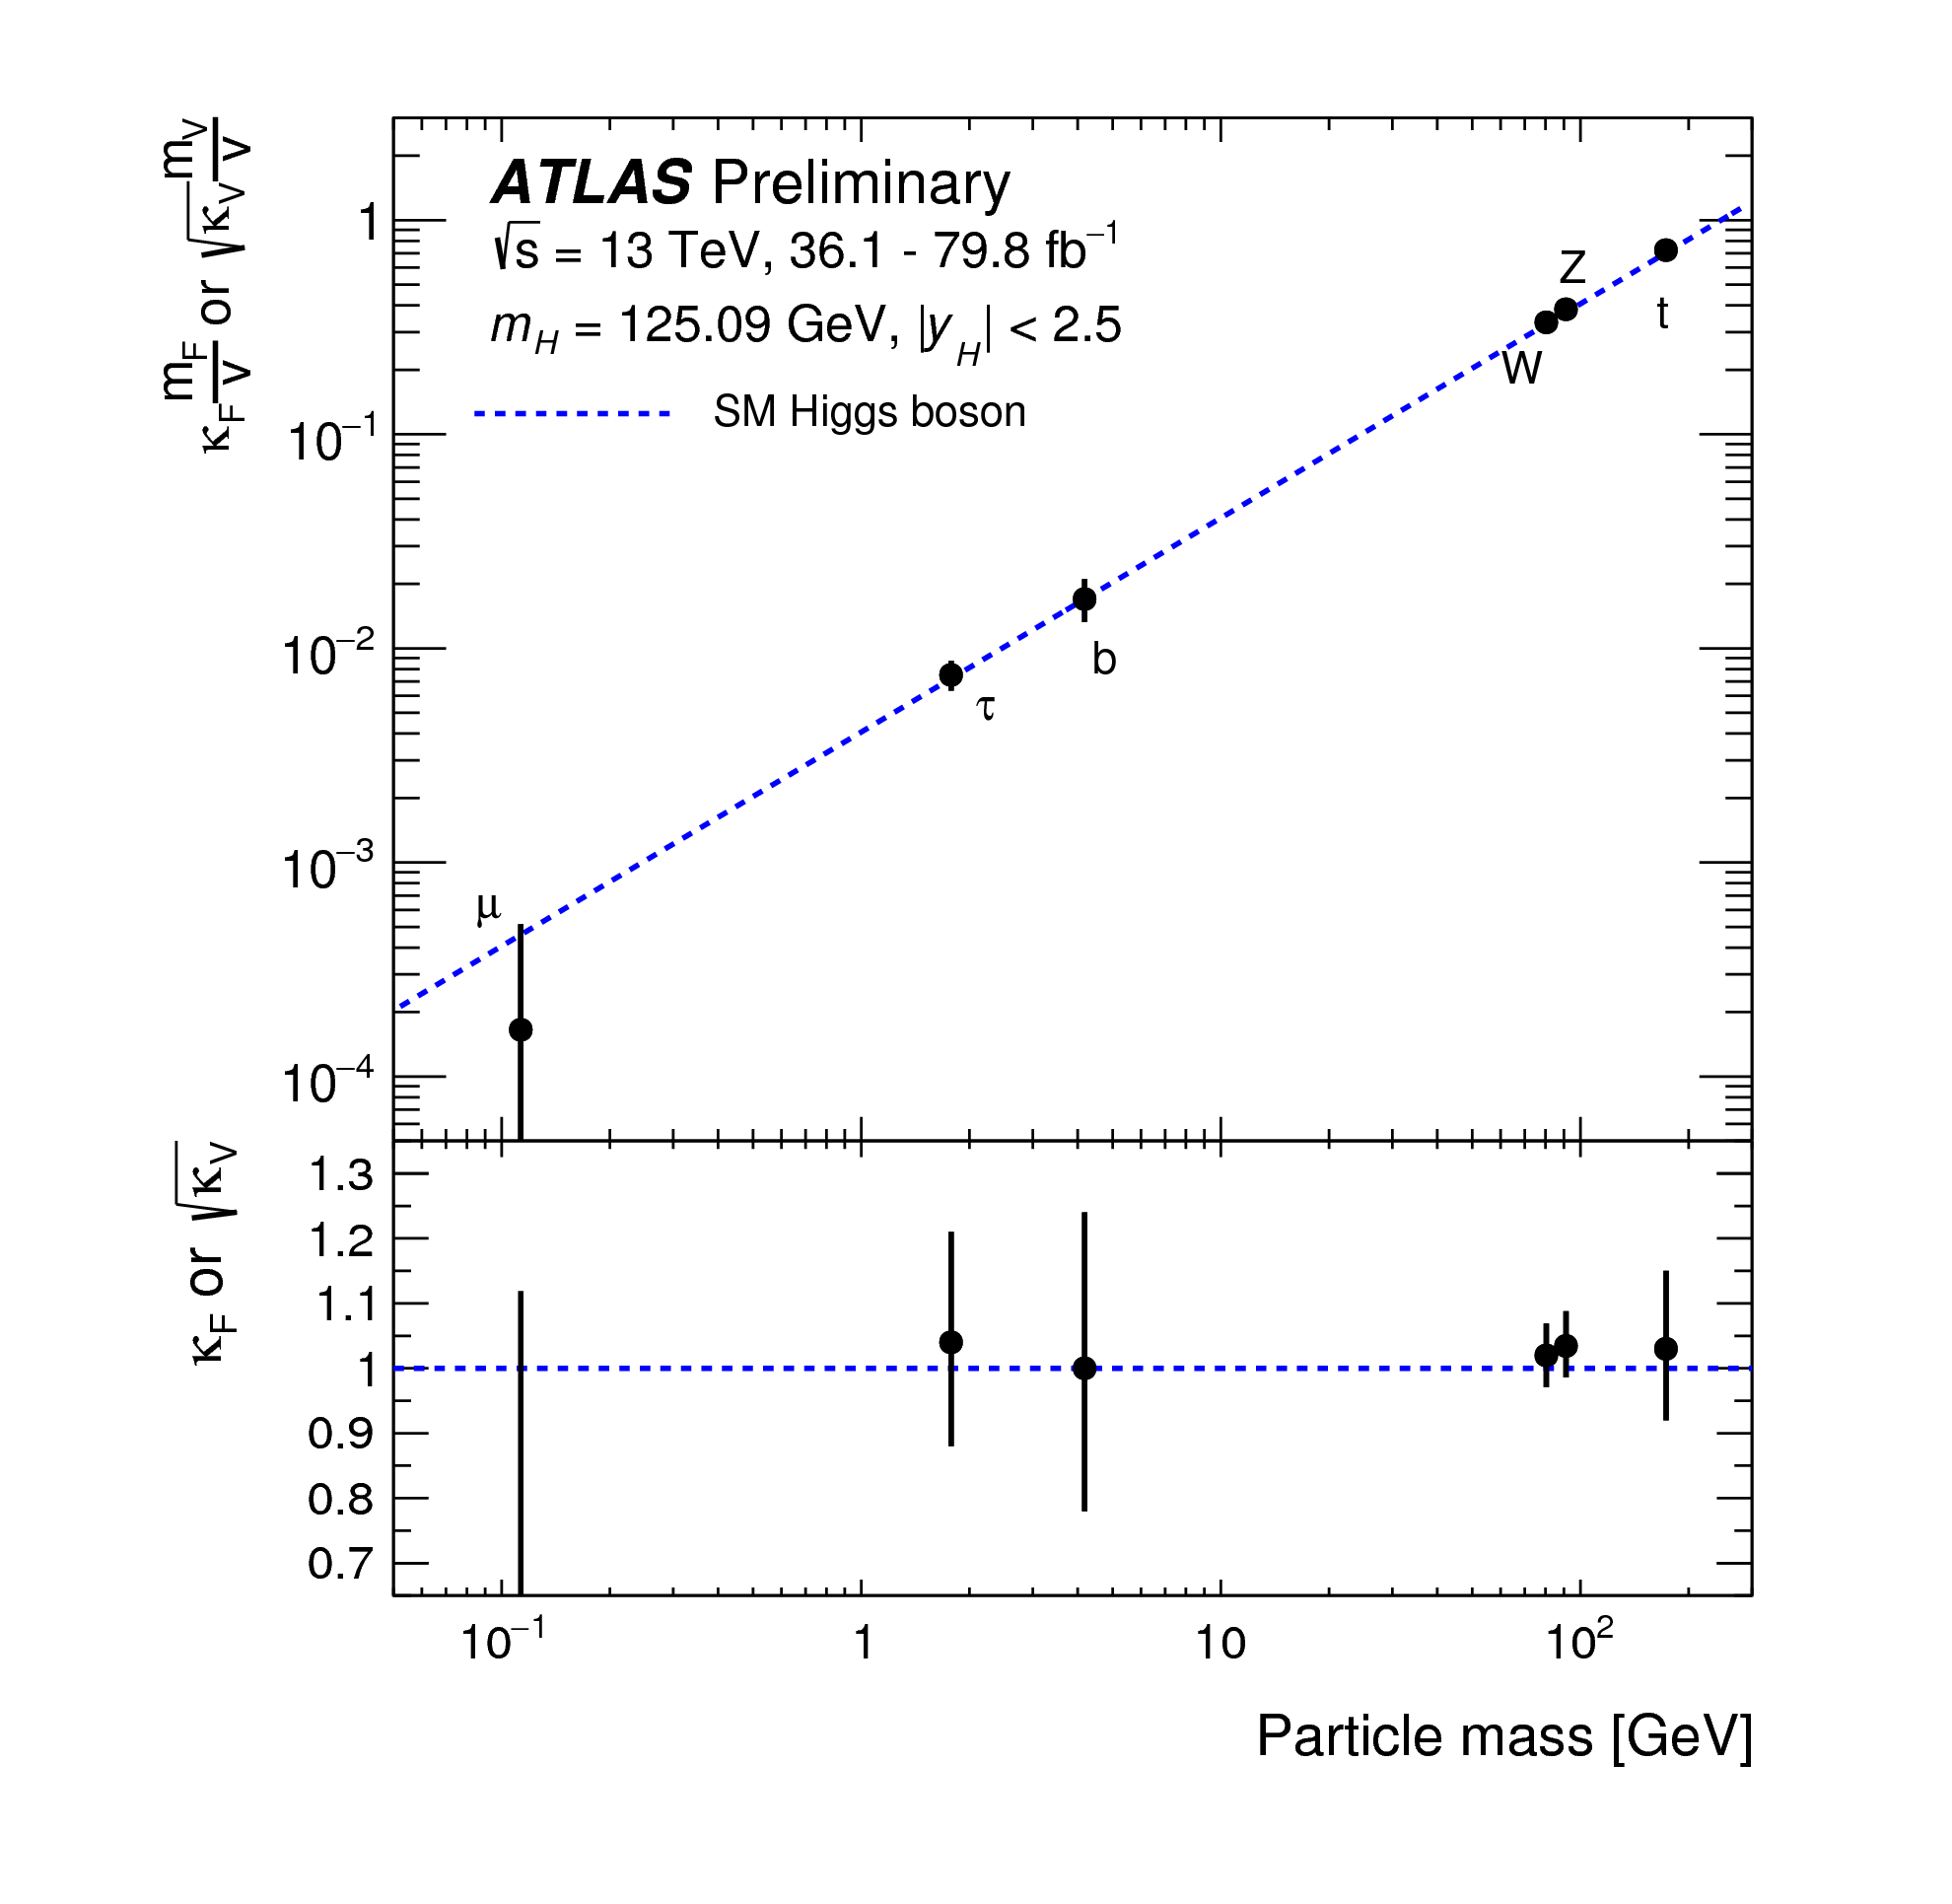
\includegraphics[height=9cm,keepaspectratio]{higgs.png}
  \caption[ヒッグス場との結合定数と素粒子の質量]{ヒッグス場との結合定数と素粒子の質量\cite{higgs}。$\kappa_\mathrm{F} m_\mathrm{F}/v$はフェルミオン($\mathrm{F}=t, b, \tau, \mu$)に対する結合定数を表し、$\kappa_\mathrm{F} m_\mathrm{F}/v$はボソン($\mathrm{V}=W, Z$)に対する結合定数を表す。$v$はヒッグス場の真空期待値を表す。 }
  \label{fig:higgs}
\end{figure}

%----------------------------------------------------------------------------
\subsection{標準模型を超えた新物理の探索\cite{evidenceDark}}
\label{sec:bsm}
%----------------------------------------------------------------------------

標準模型を用いて、これまでに行われた素粒子実験のほとんどの結果を矛盾なく説明することができる。しかし、標準模型では説明できない実験事実が確認されており、いくつかの点で不十分である。標準模型の問題の1つとして、暗黒物質が挙げられる。

暗黒物質が存在することの最も有力で直接的な実験事実は、銀河の回転曲線の測定から得られる。光学分光観測で得られる銀河全体の回転速度の分布は、銀河に含まれる星やガスから得られる物質分布から予想される回転速度よりもはるかに大きな回転速度が得られる。このことから、銀河には光学的な観測にかからない暗黒物質の存在が確認された。他にも、重力レンズ効果などの宇宙観測により、暗黒物質は宇宙全体のエネルギーの約$27\%$を占めることがわかっており、これは標準模型から得られる物質の約$6$倍の量に相当する。
暗黒物質の実態は未だわかっていないが、その候補としてWIMP(\textbf{W}eak \textbf{I}nteracting \textbf{M}assive \textbf{P}article)という、弱く相互作用する重くて安定な中性粒子が挙げられる。


暗黒物質の解明や、標準模型におけるその他の問題を解決するための新たな理論体系として、超対称性(SUSY: \textbf{Su}per \textbf{Sy}mmetry)理論がある。超対称性理論では、標準模型の全ての素粒子の対となり、スピンが$1/2$だけ異なる新たな素粒子が予言され、その中には暗黒物質の候補も含まれる。
\fref{fig:physics_bsm}に超対称性粒子と標準模型の素粒子の対応図を示す。
\begin{figure}[tbp]
  \centering
  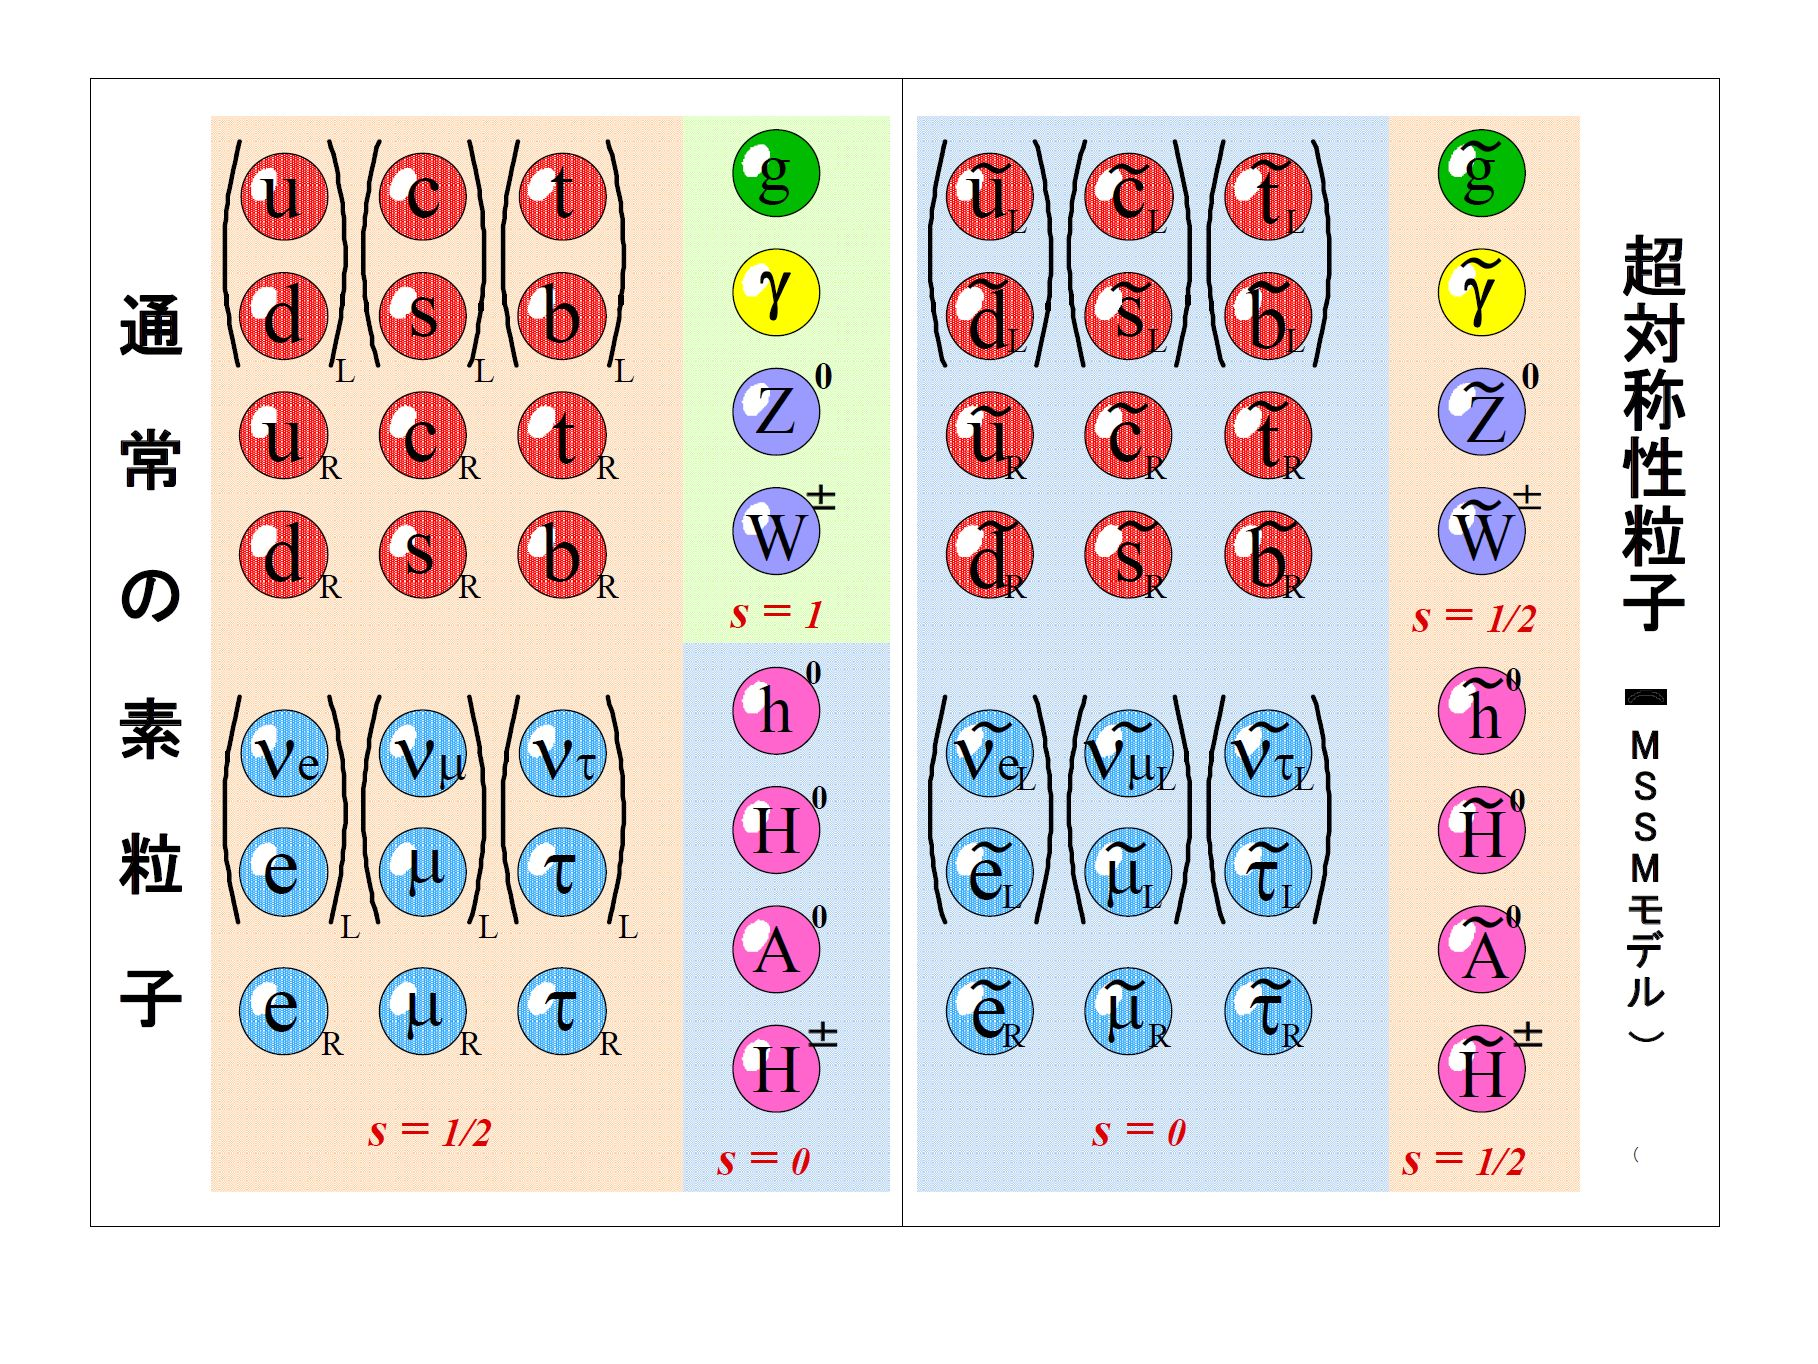
\includegraphics[height=8cm,keepaspectratio]{physics_bsm.jpg}
  \caption[超対称性粒子]{超対称性粒子 \cite{kek} }
  \label{fig:physics_bsm}
\end{figure}
超対称性粒子の中で最も軽いものをLSP(\textbf{L}ightest \textbf{S}USY \textbf{P}article)と呼ぶ。

超対称性理論は標準模型では説明が困難な問題を解決することができる一方で、バリオン数やレプトン数を破る相互作用の存在を避けることができない。バリオン数とレプトン数を破る現象のひとつとして陽子崩壊があるが、このような崩壊は観測されていない。この事実を説明するために、バリオン数とレプトン数を破る崩壊を禁止するRパリティを導入する。
Rパリティは\eref{eq:r}のように定義されている。
\begin{equation}
  \label{eq:r}
  R = (-1)^{3(B-L)}+2s
\end{equation}
ここで、$B, L$はそれぞれバリオン数、レプトン数であり、$s$はスピンである。Rパリティは標準模型の粒子では$1$となり、超対称性粒子では$-1$となる
Rパリティの保存から、標準模型の粒子と超対称性粒子に起こりうる崩壊は以下の3通りのみである。
\begin{itemize}
  \item $\mathrm{SM} \to \mathrm{SM} + \mathrm{SM}$
  \item $\mathrm{SM} \to \mathrm{SUSY} + \mathrm{SUSY}$
  \item $\mathrm{SUSY} \to \mathrm{SM} + \mathrm{SUSY}$
\end{itemize}
ここで、SMは標準模型の粒子、SUSYは超対称性粒子を表す。
超対称性粒子の中で最も軽いものであるLSP(\textbf{L}ightest \textbf{S}USY \textbf{P}article)はより軽い超対称性粒子が存在しないため、それ以上崩壊することができず安定な状態であることがわかる。したがって、中性のLSPはWIMPであり、暗黒物質の候補になりうる。
%また、重力レンズ効果等の他の宇宙観測からも暗黒物質の存在が確実視されている。


%\begin{figure}[tbp]
%  \centering
%  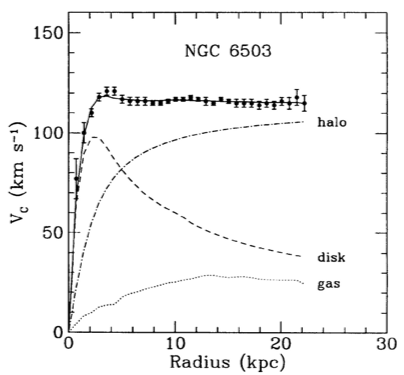
\includegraphics[height=7cm,keepaspectratio]{darkEvi.png}
%  \caption[NGC 6503 銀河の回転曲線]{ NGC 6503銀河の回転曲線 \cite{evidenceDark} }
%  \label{fig:physics_bsm}
%\end{figure}

他にも、超対称性理論の導入により、標準模型では説明できなかった問題が以下のように解決する。
\begin{itemize}
  \item 階層性問題の解決
  \item B/L対称性の破れの候補
  \item ニュートリノの質量形成のメカニズム
  \item 超ひも理論の特徴
\end{itemize}


%----------------------------------------------------------------------------
\section{LHC}
\label{sec:LHC}
%----------------------------------------------------------------------------

\begin{figure}[tbp]
  \centering
  \includegraphics[height=9cm,keepaspectratio]{LHC.jpg}
  \caption[LHCの全体図]{LHCの全体図 \cite{LHC} }
  \label{fig:LHC}
\end{figure}


LHC(\textbf{L}arge \textbf{H}adron \textbf{C}ollider)は欧州原子核研究機構(CERN)に建設された、周長がおよそ27\ \si{km}の陽子・陽子衝突型加速器である。陽子ビームの重心系エネルギーは世界最高のエネルギーである14\ \si{TeV}に到達できるよう設計されている。この世界最高のエネルギーを用いて、標準模型の精密測定やそれを超える新物理の探索がLHCの主な目的である。

\subsection{LHCの基本構造}
\fref{fig:LHC}にCERNに設置されている加速器・検出器の全体図を示す。陽子を生成し、加速器によって段階的に加速された2本の陽子ビームが、LHC周上において衝突する。


金属製の円筒に水素ガスを注入し、電場を用いて水素分子を陽子と電子に分離する。LHCのビームは、最大2808個のバンチと呼ばれる陽子のかたまりから構成され、$1.15\times 10^{11}$個の陽子が1バンチとして加速される。すなわち、LHCにおいて陽子陽子衝突から物理現象の探索をするためには、$2\ \mathrm{beams} \times 2808\ \mathrm{bunches}\times 1.15\cdot10^{11}\approx 6\cdot 10^{14}$個の陽子を生成する必要がある。

生成された陽子バンチは、初めに線形加速器 (LINAC\ 2)によって$50\ \si{MeV}$まで加速される。その後、陽子シンクロトロンブースター(PBS)、陽子シンクロトロン加速器(PS)、スーパーシンクロトロン加速器(SPS)によって段階的に$450\ \si{GeV}$まで加速され、2本の逆向きに加速された陽子バンチがLHCに投入される。LHCに投入された陽子バンチは$6.5\ \si{GeV}$(2018 年時点)まで加速されて、各衝突点において2つの陽子バンチが約$25\ \si{ns}$の間隔で衝突する。

LHCのビームパイプ上には4つの衝突点が設けられており、それぞれの衝突点において\ ATLAS(\textbf{A} \textbf{T}roidala \textbf{L}HC \textbf{A}pparata\textbf{S})、CMS(\textbf{C}ompact \textbf{M}uon \textbf{S}olenoid)、ALICE(\textbf{A} \textbf{L}arge \textbf{I}on \textbf{C}ollider \textbf{E}xperiment)、LHCb実験が行われている。




%----------------------------------------------------------------------------
\subsection{ルミノシティ}
\label{sec:luminosity}
%----------------------------------------------------------------------------

陽子ビームの強度を表すパラメータとして瞬間ルミノシティ$L$が用いられる。反応断面積$\sigma$の物理イベントが、1秒あたりに生じるイベント数 N は\eref{eq:lumi}で与えられる。
\begin{align}
  \label{eq:lumi}
  L = \gamma_{r} \frac{N_{b}^{2} n_{b} f_{rev}}{4\pi \varepsilon_{n} \beta^*}R
\end{align}
ここで、$N_{b}$は1バンチあたりに含まれる粒子数、$n_{b}$は1ビームに含まれるバンチ数、$f_{rev}$はビームの回転周波数、$\gamma_{r}$は陽子ビームのローレンツ因子、$\varepsilon_{n}$はビーム軸に垂直な平面でのビームの広がり、$\beta^{*}$は衝突点における振幅の大きさである。$R$は幾何学的損失係数という、ビーム衝突が有限の角度で起きることによる係数であり、\eref{eq:kikaf}で表される。
\begin{equation}
  \label{eq:kikaf}
  R=\left( 1+\left( \frac{\theta_{c}\sigma_{z}}{2\sigma^{*}} \right)^2 \right)^{-1/2}
\end{equation}
ここで、$\theta_c$は衝突時ビーム交差角、$\sigma_z$は衝突時におけるバンチ長の標準偏差、$\sigma^*$は衝突時におけるのバンチ幅の標準偏差である。

単位時間あたりに起こる物理事象の回数$N_\mathrm{event}$は、瞬間ルミノシティ$L$と反応断面積$\sigma$を用いて\eref{eq:hannnou}のように表すことができる。
\begin{equation}
  \label{eq:hannnou}
  N_\mathrm{event} = \int L\ dt\ \sigma
\end{equation}




%----------------------------------------------------------------------------
\section{ATLAS実験}
\label{sec:ATLAS}
%----------------------------------------------------------------------------
\begin{figure}[tbp]
  \centering
  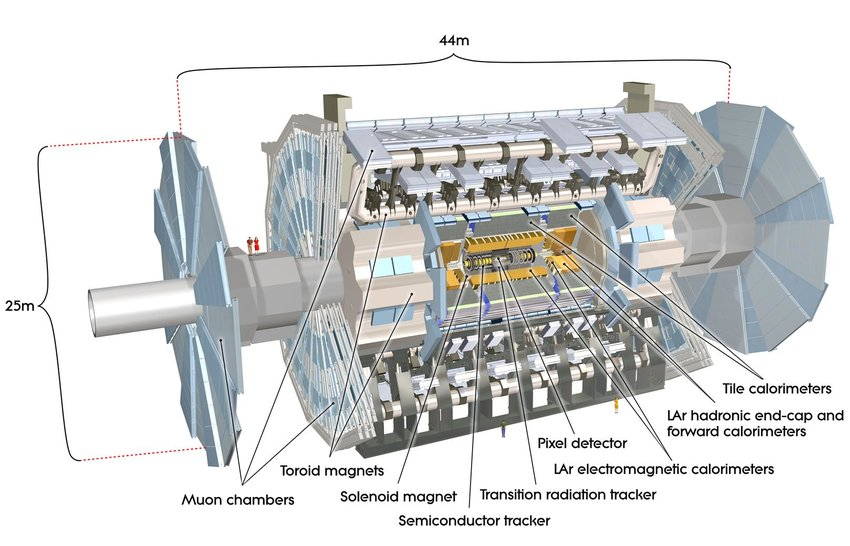
\includegraphics[height=7cm,keepaspectratio]{ATLAS.jpg}
  \caption[ATLAS検出器]{ATLAS検出器の全体図 \cite{ATLAS}。円筒の中心の内側から順に、内部飛跡検出器、電磁カロリメータ、ハドロンカロリ
  2 メータ、ミューオン検出器が衝突点を覆うように存在する。}
  \label{fig:ATLAS}
\end{figure}


ATLASはLHCの衝突点の一つに設置されている汎用型の検出器である。\fref{fig:ATLAS} に示すように、ATLAS検出器は直径25\ \si{m}長さ44\ \si{m}の円筒型をした巨大な検出器である。その中心に陽子の衝突点があり、LHCによって加速された陽子ビームが円筒の中心軸を通過するような構造になっている。
陽子ビームの衝突点である円筒の中心の内側から順に、内部飛跡検出器、電磁カロリメータ、ハドロンカロリメータ、ミューオン検出器が衝突点を覆うように存在する。内部飛跡検出器と電磁カロリメータの間にはソレノイド磁石、ハドロンカロリメータの外側にはトロイド磁石が配置されている。



%----------------------------------------------------------------------------
\subsection{ATLAS実験で使用される座標系}
\label{sec:zahyoukei}
%----------------------------------------------------------------------------
\begin{figure}[tbp]
  \centering
  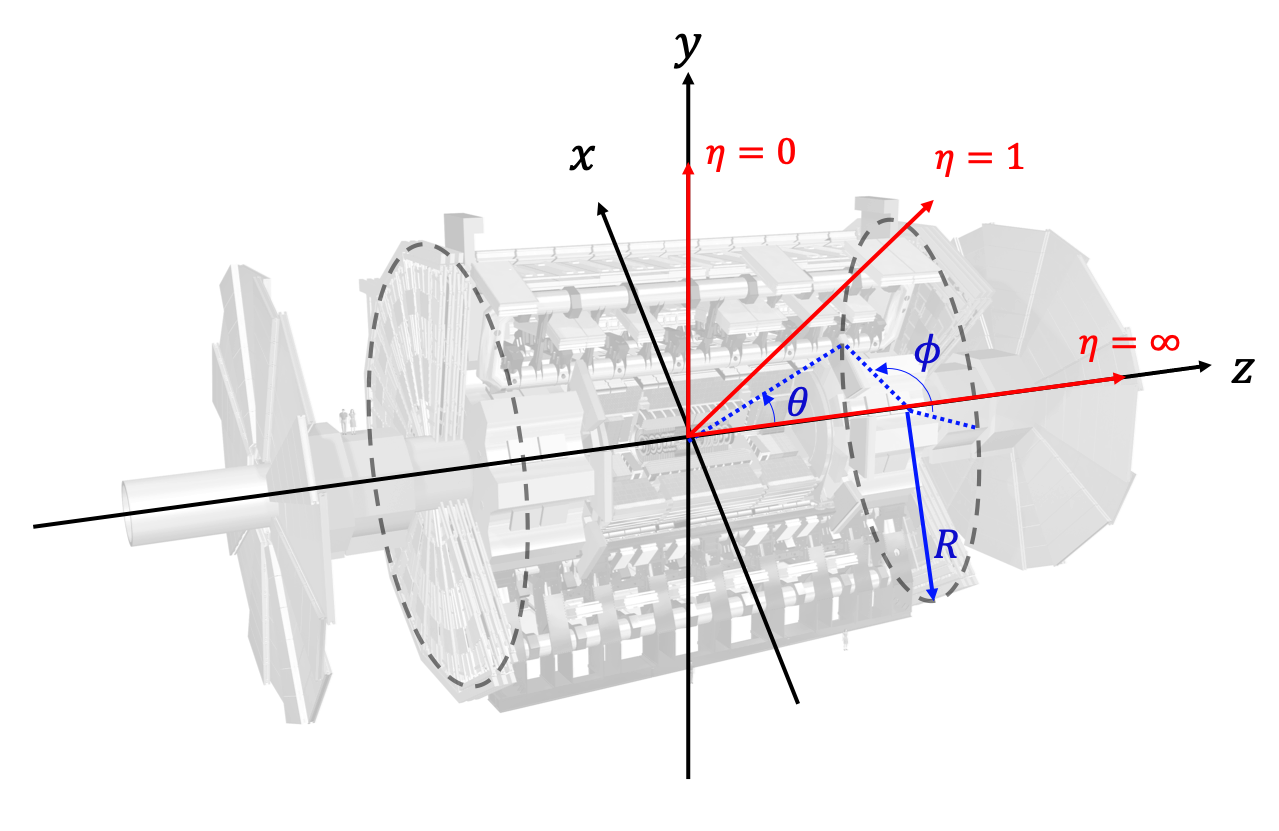
\includegraphics[height=7cm,keepaspectratio]{atlas_zahyou.png}
  \caption[ATLAS検出器]{ATLAS検出器で使用される座標系 \cite{ATLAS} }
  \label{fig:atlaszahyou}
\end{figure}

ATLASにおいて粒子の位置・運動量を示すために、\fref{fig:atlaszahyou}のような直交座標系$\left( x, y, z \right)$および円筒座標系$\left( R, \phi, z \right)$を用いる。直交座標系は陽子の衝突点を原点とし、LHCリングの中心方向を$x$軸、鉛直方向に上向きを$y$軸、ビーム軸を$z$軸と定義し、$z>0$はジュネーブ市内の方向を指す。$z$軸が正の領域をA-side、負の領域をC-sideと呼ぶ。
%\footnote{A-sideはAirportがある方向、C-sideはフランスの Saint-Genis-Pouilly という街にある Charly's Pub というバーがある方向}。
円筒座標系は$z$軸からの距離を$R$とし、$x\-y$平面内における方位角を$\phi$と定義する。また、$yz$平面における天頂角$\theta$を用いて擬ラピディティ(pesudorapidity) $\eta$を\eref{eq:eta}のように定義する。

\begin{equation}
  \label{eq:eta}
  \eta \equiv  -\ln\left( \tan{\left( \frac{\theta}{2} \right)} \right)
\end{equation}
擬ラピディティ$\eta$の差はローレンツ不変量であるため、ATLAS実験において粒子の位置や検出器の配置を示すために極角$\theta$ではなく擬ラピディティが用いられることが多い。$|\eta|$が小さくATLASの側面に対応する領域をバレル部、$|\eta|$が大きくATLASの底面に対応する部分をエンドキャップ部と呼ぶ。

%----------------------------------------------------------------------------
\subsection{内部飛跡検出器}
\label{sec:InnerDetector}
%----------------------------------------------------------------------------
\begin{figure}[tbp]
  \begin{minipage}[b]{0.45\linewidth}
    \centering
    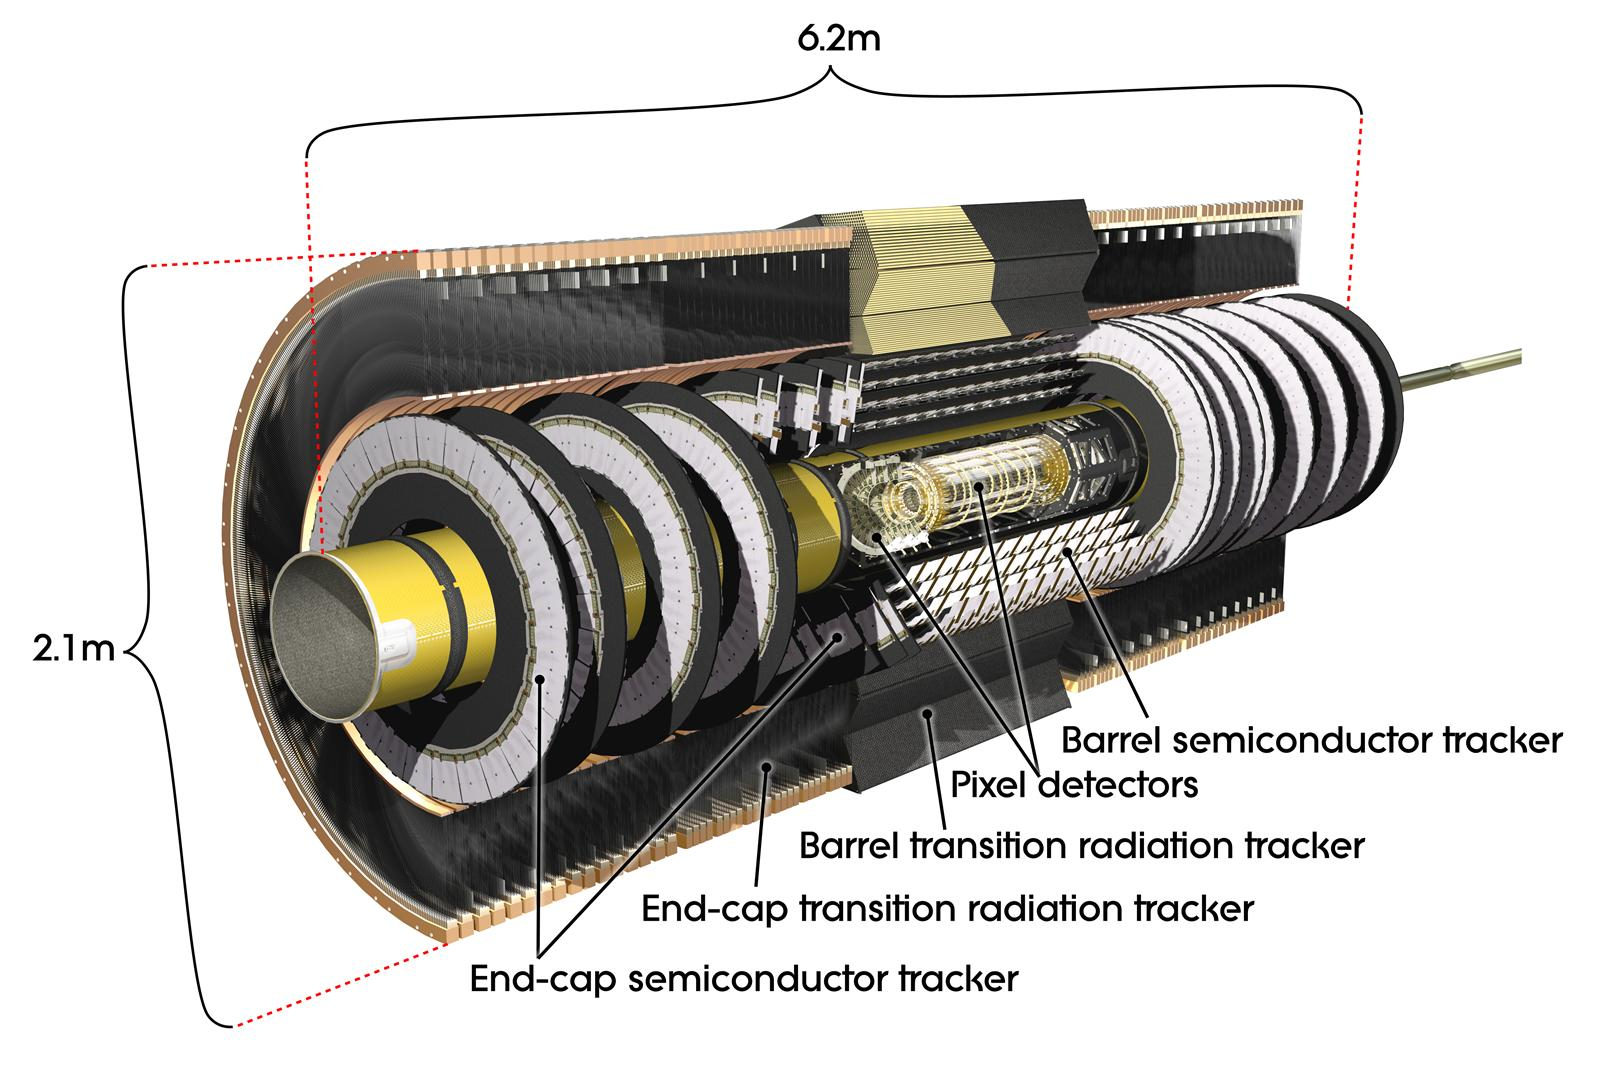
\includegraphics[keepaspectratio, scale=0.25]{InnerDetector.jpg}
    \caption{内部飛跡検出器の全体像。}
    \label{fig:InnerDetector}
  \end{minipage}
  \begin{minipage}[b]{0.45\linewidth}
    \centering
    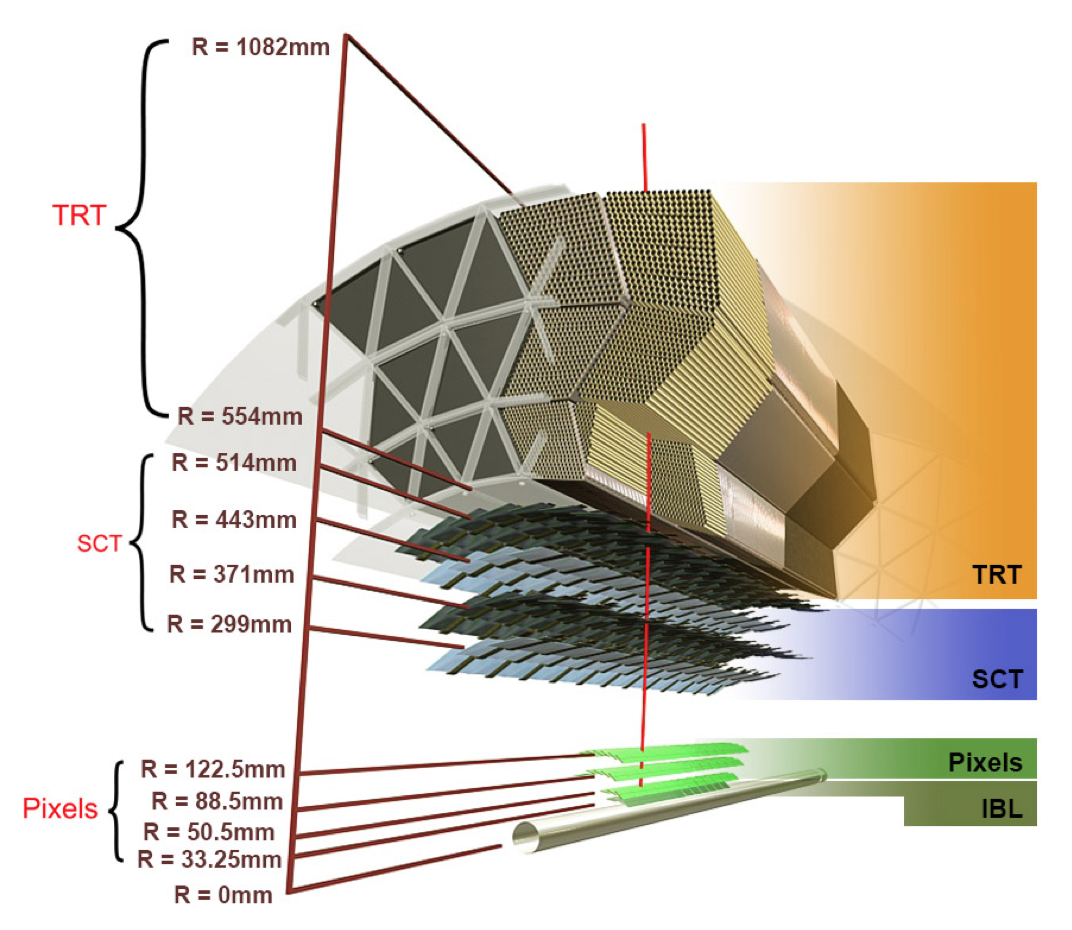
\includegraphics[keepaspectratio, scale=0.3]{structureID.png}
    \caption{内部飛跡検出器の断面図。}
    \label{fig:structureID}
  \end{minipage}
\end{figure}

\begin{figure}[tbp]
  \centering
  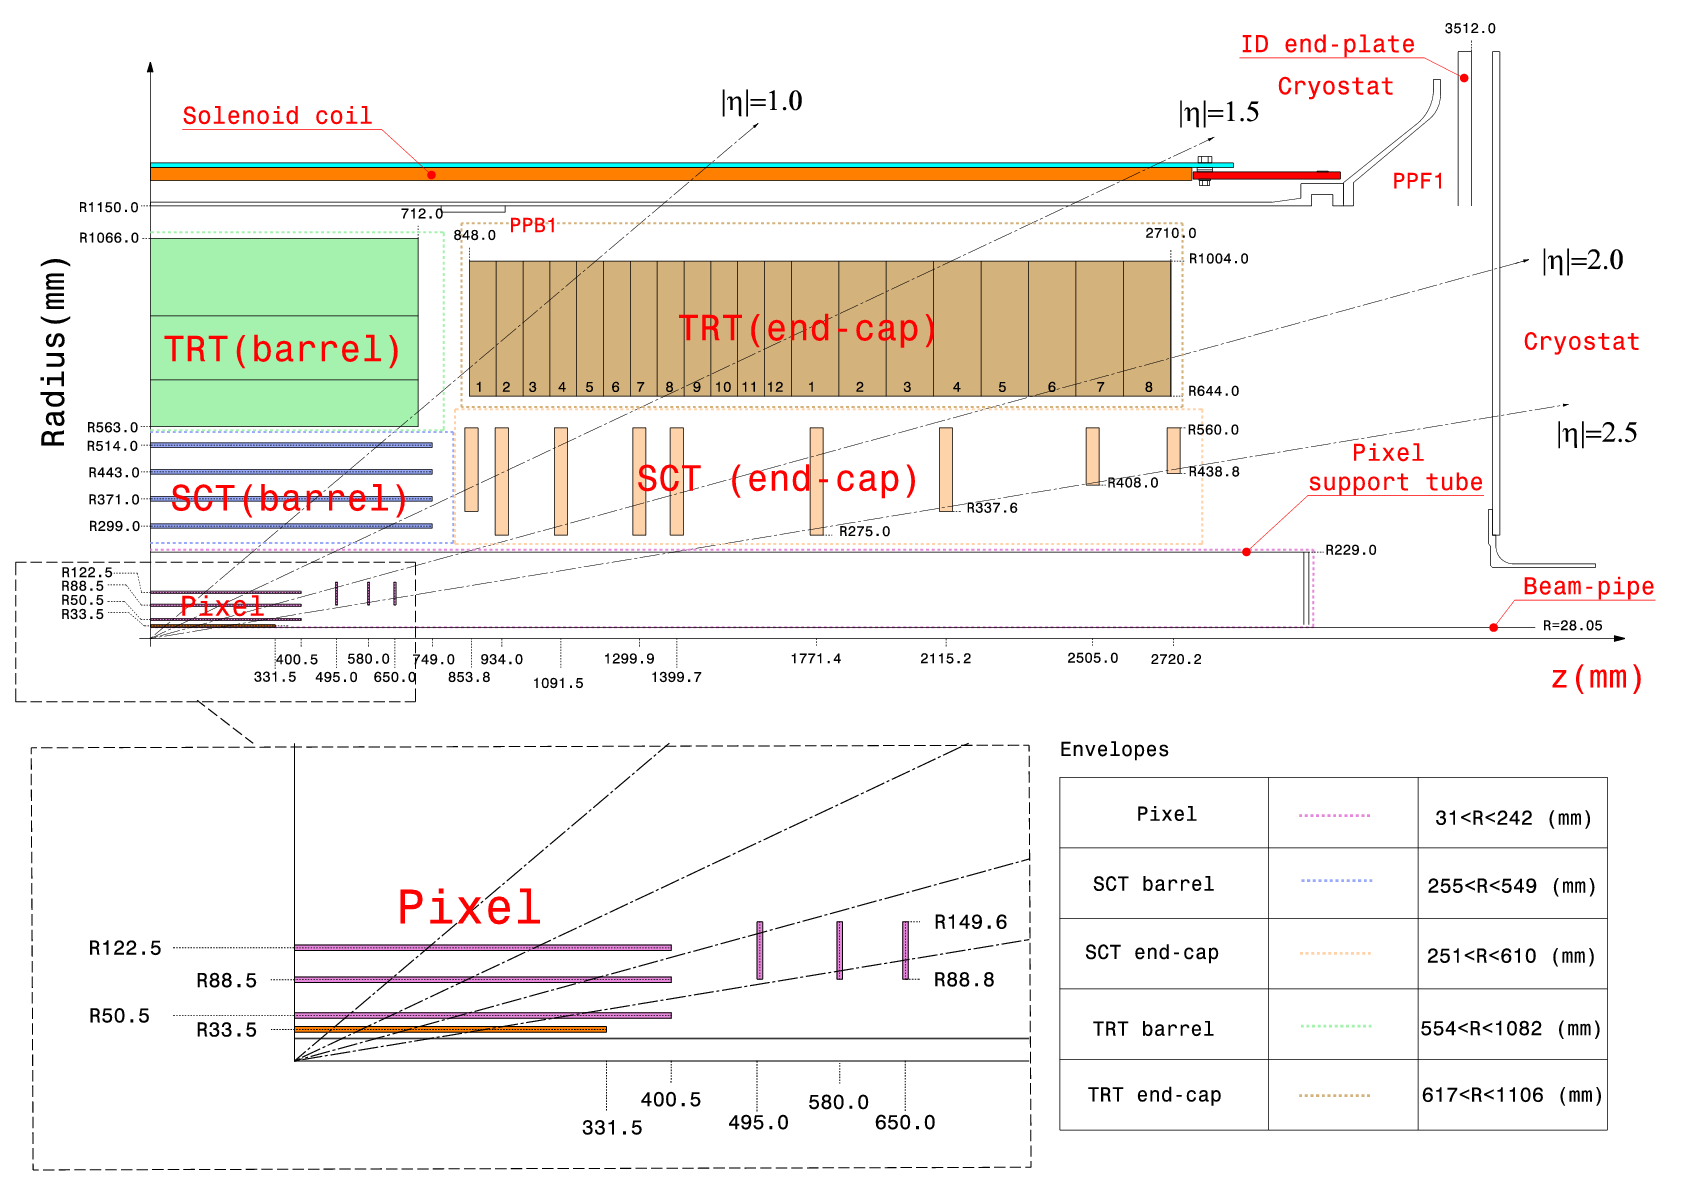
\includegraphics[height=7cm,keepaspectratio]{figures_final_pdf_NewID.png}
  \caption[内部飛跡検出器の配置]{内部飛跡検出器の配置 \cite{studyofID} }
  \label{fig:IDfigure}
\end{figure}


\fref{fig:InnerDetector}、\fref{fig:IDfigure}に内部飛跡検出器の全体図および断面図を示す。内部飛跡検出器はATLASの最内層に配置され、内側から順にIBL、ピクセル検出器、ストリップ検出器、遷移放射検出器で構成されている。衝突点から生成された荷電粒子を検出することで飛跡の再構成を行う。内部飛跡検出器の外側に配置されたソレノイド磁石により、$2\ \si{T}$の磁場がビーム軸に並行な方向にかけられる。


%----------------------------------------------------------------------------
\subsubsection{IBL、ピクセル検出器}
\label{sec:pixels}
%----------------------------------------------------------------------------

IBL(\textbf{I}nsertable \textbf{B}-\textbf{L}ayer)およびピクセル検出器はシリコン半導体検出器であり、内部飛跡検出器の最内層に配置されている。IBLはバレル部に1層配置され、ピクセル検出器はバレル部が3層、エンドキャップ部が片側3層で構成される。IBL、ピクセル検出器が配置を\tref{tab:pixel}に示す。

ピクセル検出器はLHCの運転開始時である2007年から稼働している検出器であり、読み出しチップにFE-I3という$50\times400\ \si{\micro m^2}$のピクセルを持つASICが使用されている。
IBLは、LHCにおける2年間のシャットダウン期間(2012年 - 2014年)に新たに設置された。IBLは陽子ビームの衝突点に最も近い検出器のため、高い放射線耐性と多い事象数を処理することができるように設計されている。読み出しチップにはFE-I4と呼ばれる、$50\times250\ \si{\micro m^2}$のピクセルを持つASICが使用されている。これらのASICの詳細については\ref{sec:genkoupixel}節に示す。

\begin{table}[htbp]
  \begin{center}
    \caption[IBL、ピクセル検出器の配置]{IBL、ピクセル検出器の配置}
    \label{tab:pixel}
    \begin{tabular}{|c||c|c|c|c|c|}
    \hline
       &  & $R\ [\si{mm}]$ & $z\ [\si{mm}]$ & 検出器の総数 & ピクセルの総数$(\times 10^{6})$ \\
    \bhline{1.5pt}
    \multirow{4}{*}{Barrel}
     & IBL & $33.5$ & $ < 331.5$ & $224$ & $6.02$ \\
     \cline{2-6}
     & B-layer & $50.5$ & $< 400.5$ & $286$ & $13.2$ \\
     \cline{2-6}
     & Layer 1 & $88.5$ & $< 400.5$ & $494$ & $22.8$ \\
     \cline{2-6}
     & Layer 2 & $122.5$ & $< 400.5$ & $676$ & $31.2$ \\
    \hline
    \multirow{3}{*}{Endcaps}
     & Disk 1 & $88.8 < R < 149.6$ & $495$ & $48\times2$ & $4.4$ \\
     \cline{2-6}
     & Disk 1 & $88.8 < R < 149.6$ & $580$ & $48\times2$ & $4.4$ \\
     \cline{2-6}
     & Disk 1 & $88.8 < R < 149.6$ & $650$ & $48\times2$ & $4.4$ \\
    \hline
    \end{tabular}
  \end{center}
\end{table}



%----------------------------------------------------------------------------
\subsubsection{ストリップ検出器}
\label{sec:sct}
%----------------------------------------------------------------------------
ストリップ検出器(SCT: \textbf{S}emi\textbf{C}onductor \textbf{T}racker)はシリコン半導体検出器であり、ピクセル検出器の外側に配置されている。バレル部4層で$|\eta|<1.4$の領域を、エンドキャップ部では片側9層ずつで$1.4<|\eta|<2.5$の領域を覆うように配置されている。
ストリップ検出器のモジュールはストリップが$80\ \si{\micro m}$間隔で並んだシリコンセンサー2枚を$40\ \si{m rad}$ずらして重ねることにより、入射粒子の二次元の位置情報を測定することができる。



%----------------------------------------------------------------------------
\subsubsection{遷移放射検出器}
\label{sec:trt}
%----------------------------------------------------------------------------
遷移放射検出器(TRT: \textbf{T}ransition \textbf{R}adiation \textbf{T}racker)は、ストローチューブで構成された検出器であり、内部飛跡検出器の最外層に配置されている。バレル部では$52544$本のストローチューブ(長さ$1.5\ \si{m}$)が$0.5\ \si{m} < R < 1.1\ \si{m},\ |\eta|<1$の領域を、エンドキャップ部では片側$122880$本のストローチューブ(長さ$0.4\ \si{m}$)が$0.8\ \si{m} < |z| < 2.7\ \si{m},\  < |\eta| < 2$の領域を覆うように配置されている。ドリフトチューブの直径は$4\ \si{mm}$であり、チューブ内部には$70\%$のXe、$27\%$のCO$_{2}$と$3\%$のO$_{2}$の混合ガスが充填されており、チューブの中心部に直径$31\ \si{\micro m}$のワイヤーが張られている。荷電粒子がストローチューブを通過すると、混合ガスをイオン化する。それにより発生した自由電子は、チューブの外側にかけられた電場によりワイヤーに向かってドリフトし、読み出しされる。



%----------------------------------------------------------------------------
\subsection{カロリメータ}
\label{sec:calocalo}
%----------------------------------------------------------------------------
\begin{figure}[tbp]
  \centering
  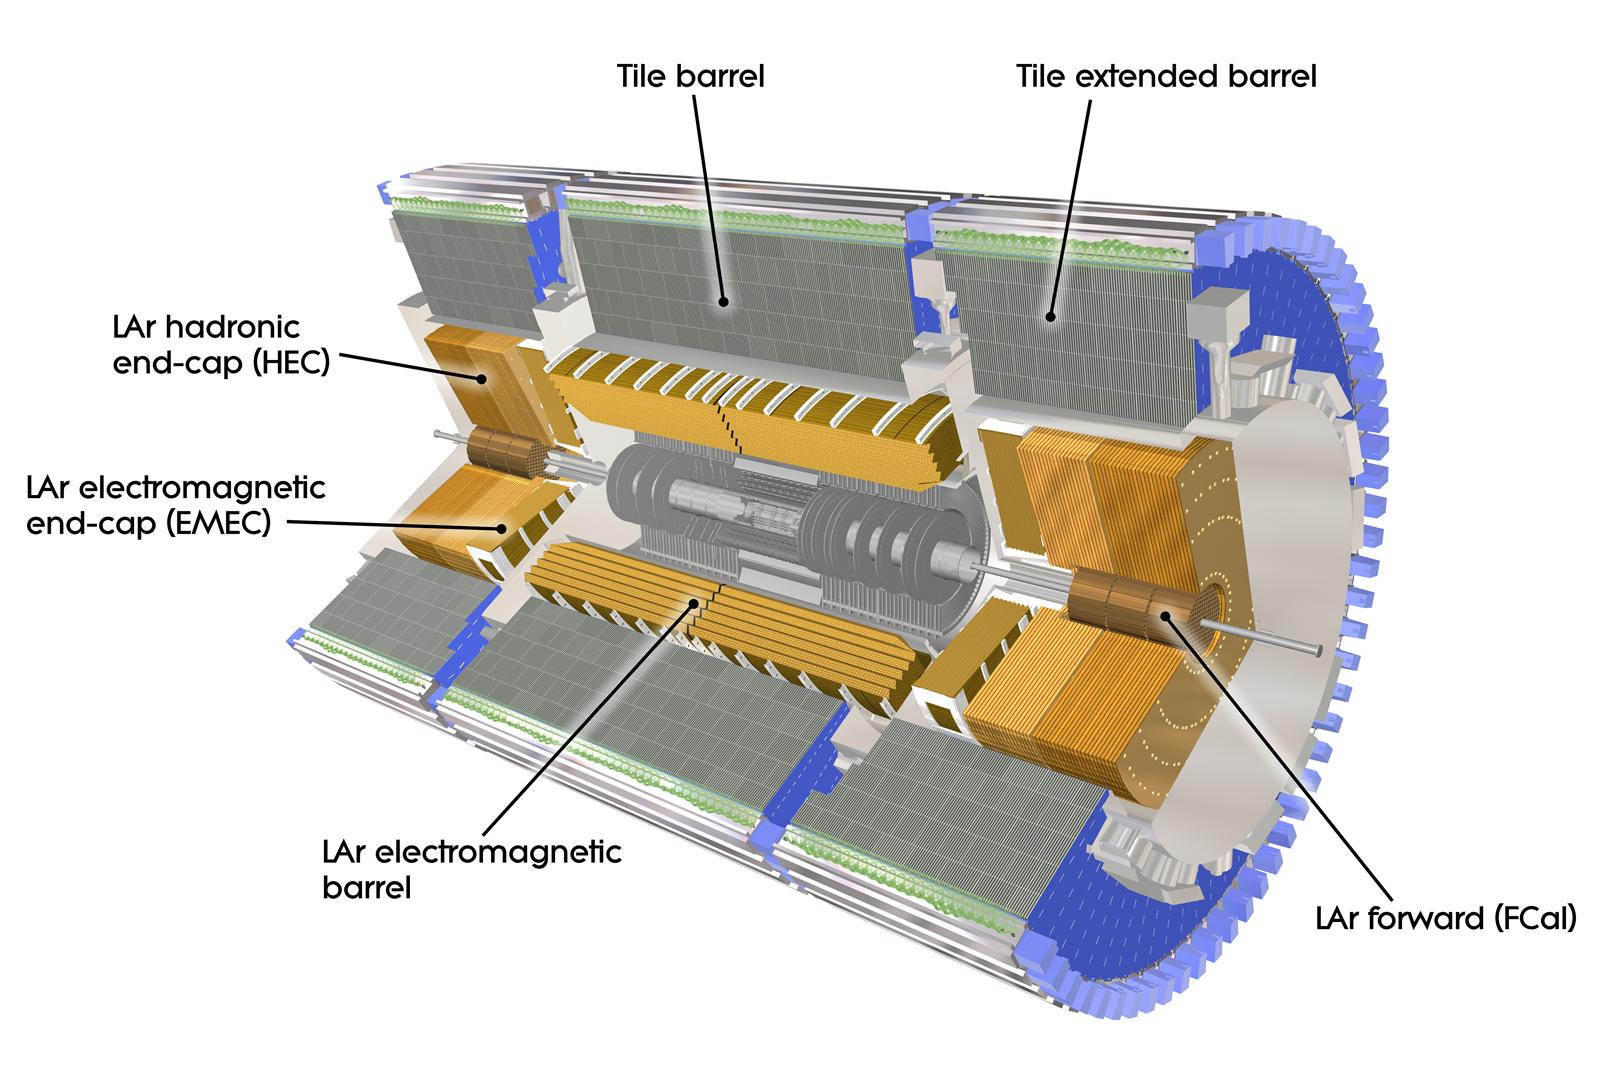
\includegraphics[height=7cm,keepaspectratio]{calocalo.jpg}
  \caption[ATLASカロリメータ]{カロリメータの全体図 \cite{calocalo} }
  \label{fig:calocalo}
\end{figure}

\fref{fig:calocalo}にカロリメータの全体像を示す。ATLASにおけるカロリメータはサンプリング型のカロリメータであり、検出層と吸収層から成る積層構造である。カロリメータは内部飛跡検出器の外側に配置されており、全体で$|\eta|<4.9$の領域を覆うように配置されている。粒子と物質の相互作用の違いから、対象とする粒子の種類により電磁カロリメータとハドロンカロリメータが用意されている。このような構造から、カロリメータを用いて通過粒子のエネルギーや位置の測定、電子・光子とハドロンの区別、ジェットの識別を行うことができる。

電磁カロリメータは、ソレノイド磁石の外側のバレル部($|\eta|<1.4$)とエンドキャップ部($1.4<|\eta|<3.2$)の領域に設置されている。検出層に液体アルゴン\footnote{液体アルゴン(LAr)はエネルギー応答が線形で且つ安定を持つ物質である。また、放射線耐性も充分持ち合わせている。}、吸収層に鉛($\mathrm{Z}=82$)が用いられており、高エネルギーの電子・光子が電磁カロリメータに到達すると、吸収層において電子対生成や制動放射を繰り返し、電磁シャワーを形成する。低エネルギーになった粒子は検出層においてイオン化しエネルギーを失い、イオン化により発生した電子が電気信号として読み出される。電磁シャワーによって得られる合計エネルギーを計算することにより、入射電子・光子のエネルギー測定を行うことができる。電子と光子の区別は、内部飛跡検出器中の飛跡情報を用いて行う。
電磁カロリメータの厚さは$20X_0$\footnote{$X_0$は放射長であり、入射粒子のエネルギーが$1/e\sim0.37$となる距離である。}を超えるため、測定対象である電子・光子のほとんどは電磁カロリメータにおいて全てのエネルギーを失う。

ハドロンカロリメータは、電磁カロリメータの外側にあり、バレル部($|\eta|<1.7$)とエンドキャップ部($1.5<|\eta|<3.2$)の領域に設置されている。バレル部は検出層にシンチレータ、吸収体に鉄を用いたタイルカロリメータから成り、エンドキャップ部では検出層に液体アルゴン、吸収層に銅が用いられる。高エネルギーのハドロンがハドロンカロリメータに入ると、吸収層において原子核と強い相互作用し粒子多重生成を行い、カスケードシャワーを発生しそのエネルギー測定を行う。



%----------------------------------------------------------------------------
\subsection{ミューオン検出器}
\label{sec:mumu}
%----------------------------------------------------------------------------
ミューオン検出器はカロリメータの外側にあり、$|\eta|<2.7$の領域に設置される、ATLASにおける最外層の検出器である。ミューオンは物質の透過力が高く、他の崩壊生成粒子と比較して寿命が長い($\sim 2.2\ \si{\micro sec}$)ため、ATLASの外側まで透過する。予想される最高エネルギー($1\ \si{TeV}$)までのミューオンの運動量を測定できるよう設計されている。

ミューオン検出器の大部分は、MDT(\textbf{M}onitored \textbf{D}rift \textbf{T}ube)である。MDTは直径約$3\ \si{cm}$のドリフトチューブ検出器であり、ミューオンの通過位置を測定することができる。測定のトリガーとして、バレル部においてはRPC(\textbf{R}esistive \textbf{P}late \textbf{C}hamber)、エンドキャップ部においてはTGC(\textbf{T}hin \textbf{G}ap \textbf{C}hamber)から得られる情報を用いる。ビームパイプに近い領域($2.0<|\eta|<2.7$)においては、バックグラウンドの$\gamma$線や中性子が多く,ヒットレートが大きい。MDTはドリフト時間が長いため、この領域においてはMDTではなく高い入射レートに耐えられるCSC(\textbf{C}athode \textbf{S}trip \textbf{C}hamber)を用いてミューオンの通過位置測定を行う。







%----------------------------------------------------------------------------
\section{HL-LHCアップグレード}
\label{sec:HL-LHC}
%----------------------------------------------------------------------------
\begin{figure}[tbp]
  \centering
  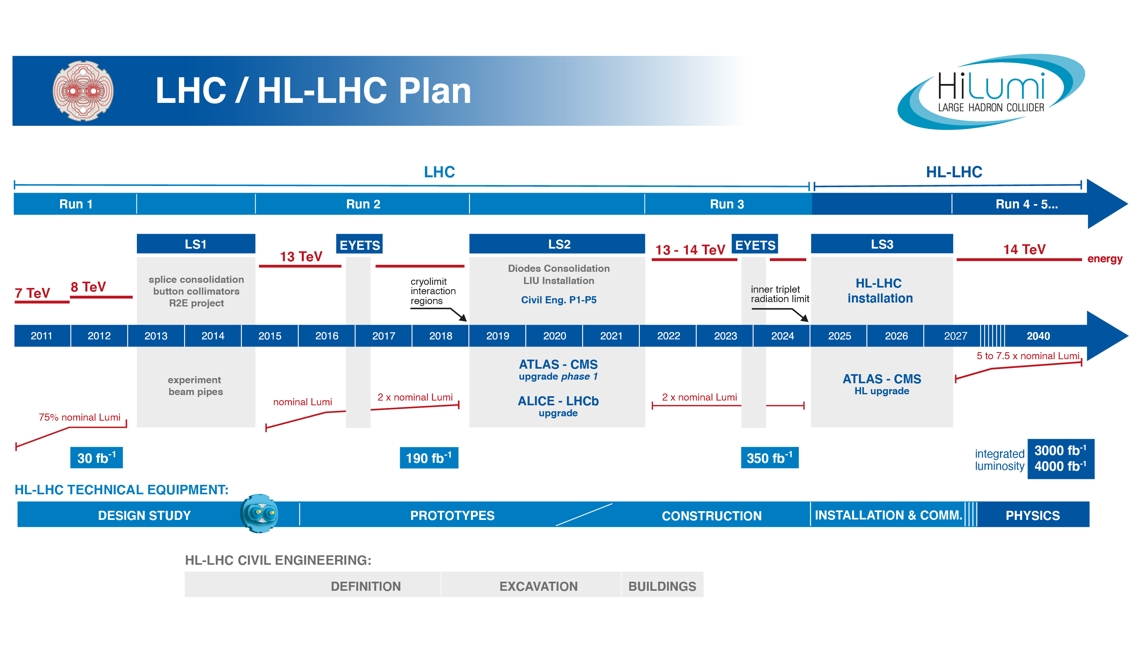
\includegraphics[height=8cm,keepaspectratio]{HL-LHC-January-2021_small.jpg}
  \caption[LHCの運転計画]{2021年1月に作成されたLHCの運転計画 \cite{hl-lhc}。2025年 }
  \label{fig:hl-lhc}
\end{figure}

\fref{fig:hl-lhc}にLHCの運転計画を示す。LHCでは、2025年から\textbf{HL-LHC}(High Luminosity LHC)アップグレードが開始する予定である。2027年の運転開始から瞬間ルミノシティを設計値である$1.0\times 10^{34}\ \si{cm^{-2}s^{-1}}$の$5 \mathchar`- 7$倍に増加させ、2037年における運転停止までの積分ルミノシティをRun3までで取得予定である$300\ \si{fb^{-1}}$の約$10$倍にまで増加させることが目標である。

このアップグレードに伴い、ATLASに配置される検出器についてもアップグレードが予定されている。この節では、HL-LHCアップグレード計画と、本研究と関わりのあるATLAS内部飛跡検出器のアップグレード計画について述べる。

%----------------------------------------------------------------------------
\subsection{HL-LHCの概要}
\label{sec:HL-LHC-gaiyou}
%----------------------------------------------------------------------------
%\begin{figure}[tbp]
%  \centering
%  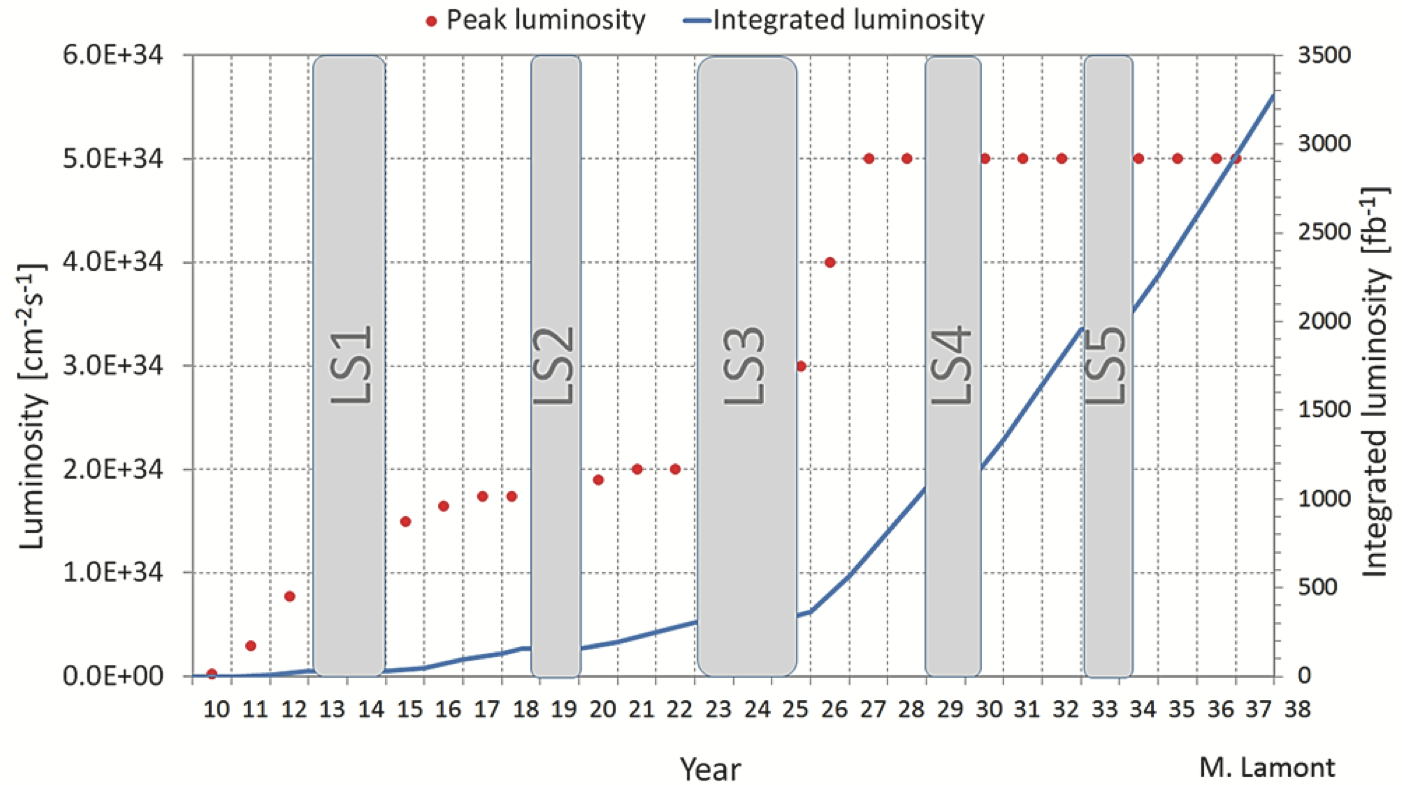
\includegraphics[height=7cm,keepaspectratio]{time_lumi.png}
%  \caption[LHCのピークルミノシティと積分ルミノシティ]{ \cite{lhc-lumi}}
%  \label{fig:time-lumi}
%\end{figure}

\begin{table}[htbp]
  \begin{center}
    \caption[HL-LHCでのビームパラメータ]{HL-LHCでのビームパラメータ\cite{lhc-lumi}}
    \label{tab:genkou-hl}
    \begin{tabular}{|l||c|c|}
    \hline
      パラメータ & 現行LHC & HL-LHC \\
    \bhline{1.5pt}
    陽子エネルギー [\si{TeV}] & 7 & 7 \\
    \hline
    1バンチあたりの陽子数 $N_b$ & $1.15\times 10^{11}$ & $2.2\times 10^{11}$ \\
    \hline
    交差角$\theta_c\ [\si{\micro rad}]$ & 285 & 590 \\
    \hline
    幾何学的損失係数$R$(括弧内はクラブ空洞無し) & 0.836 & 0.829 (0.305) \\
    \hline
    衝突点における振幅$\beta^*\ [\si{m}]$ & 285 & 590 \\
    \hline
    $xy$平面のビームの広がり$\varepsilon_n\ [\si{\micro m}]$ & 3.75 & 2.50 \\
    \hline
    1交差あたりの事象数(パイルアップ) & 27 & 138 \\
    \hline
    パイルアップ密度[$\si{/mm}$] & 0.21 & 1.25 \\
    \hline
    積分ルミノシティ[$\si{fb^{-1} /year}$] & 45 & 260 \\
    \hline
    \end{tabular}
  \end{center}
\end{table}

LHCは2010年春から本格運転を開始し、長期運転停止期間(LS: \textbf{L}ong \textbf{S}hutdown)を重ねて、ピークルミノシティを設計値である$1.0\times 10^{34}\ \si{cm^{-2}s^{-1}}$の$2$倍まで向上させ、データ取得を行っていく予定である。さらに、2025年-2027年における長期運転停止期間(LS3)においてLHCのアップグレードを行い、瞬間ルミノシティを現行LHCの設計値の$5 \mathchar`- 7$倍にまで増加させる。

\tref{tab:genkou-hl}に現行LHCとHL-LHCで予定されている主なビームパラメータをまとめる。
\eref{eq:lumi}より、瞬間ルミノシティを増大させるには、ビーム電流($N_b, n_b$)を増強し、衝突点でのビームサイズ($\varepsilon_n, \beta^*$)を絞り、交差角$\theta_c$による幾何学的損失係数$R$をできるだけ大きくするよう設計する必要がある。そのため、HL-LHCではルミノシティを大幅に向上させるために以下のような改良を計画している。
\begin{itemize}
  \item LHCに入射する陽子ビームの強度と輝度を向上させるため、前段加速器の各機器(Linac4, PSB, PS, SPS)について更新・アップグレードを実施
  \item 衝突点でのビームサイズを絞る(衝突点における振幅$\beta^*$を減少)ため、ATLAS、CMSの衝突点周りの挿入部に新たに高磁場の磁石を実装
  \item 幾何学的損失係数$R$を現行LHCと同程度に保つため、衝突点のクラブ空洞\footnote{「クラブ空洞」とは、高エネルギー加速器研究機構(KEK)で開発された特殊な超伝導空洞で、電子・陽電子ビームのバンチを回転させることにより、より高いルミノシティを達成することを目指して開発された技術である。\cite{crab}}を導入
\end{itemize}






%----------------------------------------------------------------------------
\subsection{内部飛跡検出器のアップグレード}
\label{sec:hl-lhc-itk}
%----------------------------------------------------------------------------
HL-LHCにおいて、ATLASはこれまでよりもさらに過酷な放射線環境下に晒される。瞬間ルミノシティが現行LHCの設計値の$5 \mathchar`- 7$倍にまで増加するため、現行のATLASを用いてHL-LHCの環境下において測定を行うと主に二つの問題が生じると予想される。
\begin{itemize}
\item 瞬間ルミノシティが大きくなることにより、バンチ衝突あたりの生成粒子数が増加し放射線損傷の影響がより大きくなる。検出器のセンサーが放射線損傷を受けると、検出効率が低下するため、より高い放射線耐性を持つ検出器が要求される。
\item 各検出器のヒット占有率の増加である。HL-LHCでは、パイルアップが$200$まで増加すると予想されており内部飛跡検出器での飛跡の数が増加することで、飛跡の識別が困難になり、再構成の性能が大幅に低下する。特に、荷電粒子への感度が高いガス検出器であるTRTでは検出器の占有率が$100\si{\%}$に達してしまうと予想されている。そのため、HL-LHCにおいてはよりパイルアップ耐性が高い検出器が必要となる。
\end{itemize}
%これらの問題により、ピクセル検出器に対する要求は\tref{tab:hlVSIBL}となっている。放射線耐性について$1\ \si{MeV}$の中性子換算で$1.4\times 10^{16}\ \si{n_{eq}/cm^2}$という。また、位置分解能向上およびヒット占有率の増加を防ぐため、ピクセルサイズは現行IBLの$1/5$になっている。

\begin{table}[htbp]
  \begin{center}
    \caption[HL-LHCでのビームパラメータ]{HL-LHCでのビームパラメータ\cite{lhc-lumi}}
    \label{tab:genkou-hl}
    \begin{tabular}{|l||c|c|}
    \hline
      パラメータ & 現行IBL & ITk \\
    \bhline{1.5pt}
    ピクセルサイズ [$\si{\micro m^2}$] & 7 & 7 \\
    \hline
    読み出しデータレート $N_b$ & $1.15\times 10^{11}$ & $2.2\times 10^{11}$ \\
    \hline
    交差角$\theta_c\ [\si{\micro rad}]$ & 285 & 590 \\
    \hline
    幾何学的損失係数$R$(括弧内はクラブ空洞無し) & 0.836 & 0.829 (0.305) \\
    \hline
    衝突点における振幅$\beta^*\ [\si{m}]$ & 285 & 590 \\
    \hline
    $xy$平面のビームの広がり$\varepsilon_n\ [\si{\micro m}]$ & 3.75 & 2.50 \\
    \hline
    1交差あたりの事象数(パイルアップ) & 27 & 138 \\
    \hline
    パイルアップ密度[$\si{/mm}$] & 0.21 & 1.25 \\
    \hline
    積分ルミノシティ[$\si{fb^{-1} /year}$] & 45 & 260 \\
    \hline
    \end{tabular}
  \end{center}
\end{table}


\begin{figure}[tbp]
  \centering
  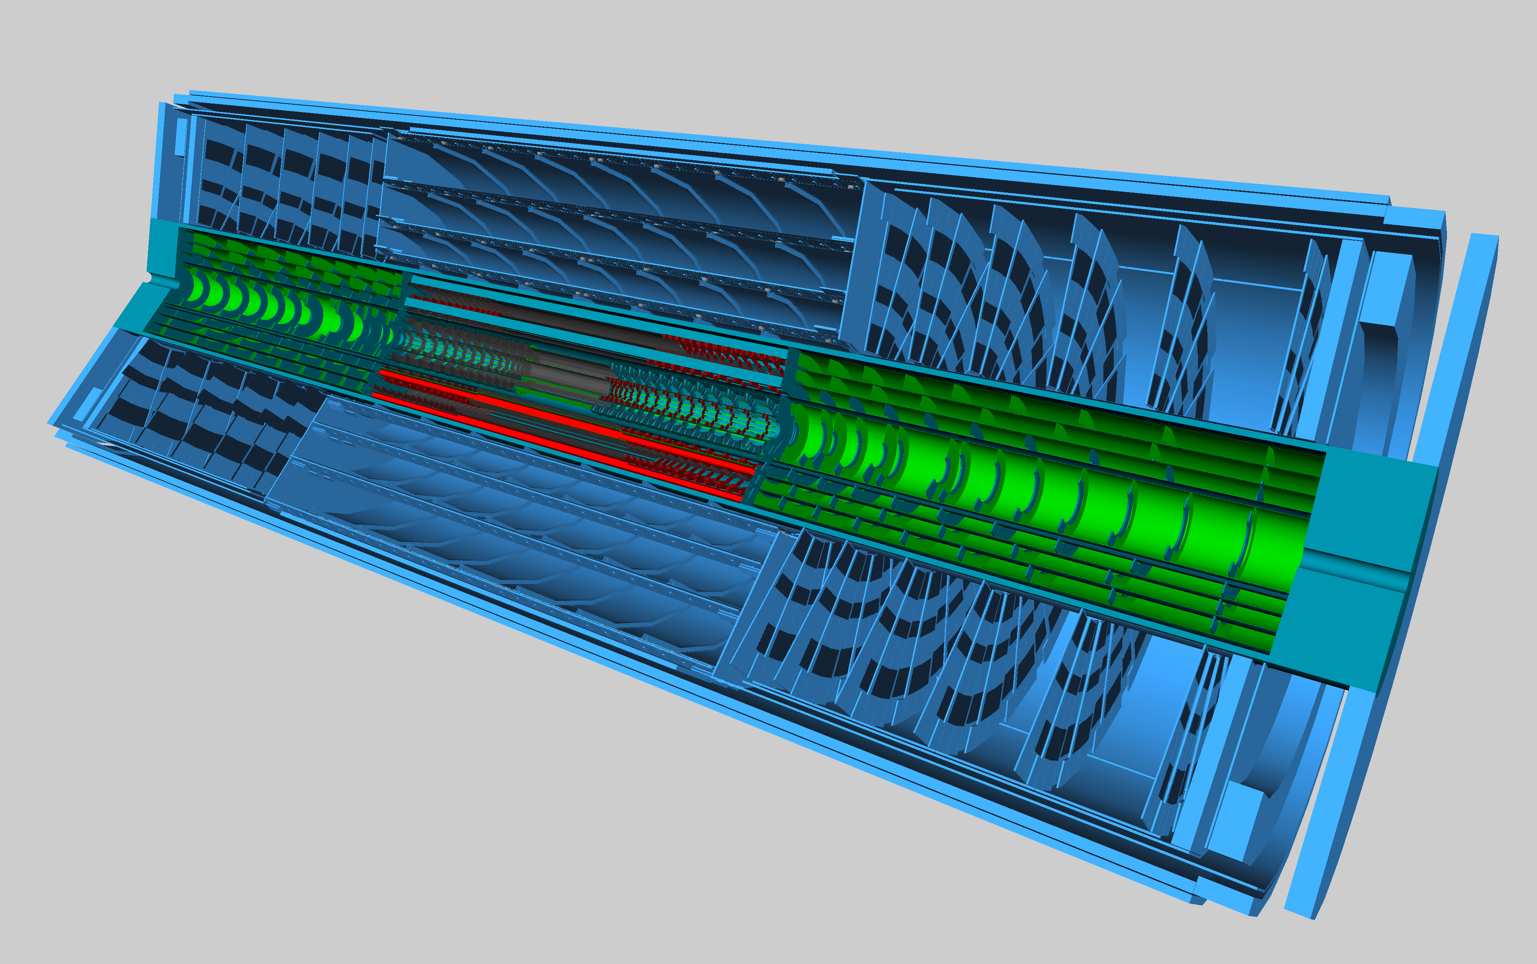
\includegraphics[height=8cm,keepaspectratio]{itk_display.png}
  \caption[ITkの断面図]{ITkの断面図 \cite{itk}。}
  \label{fig:hl-lhc-itk}
\end{figure}

\begin{figure}[tbp]
  \centering
  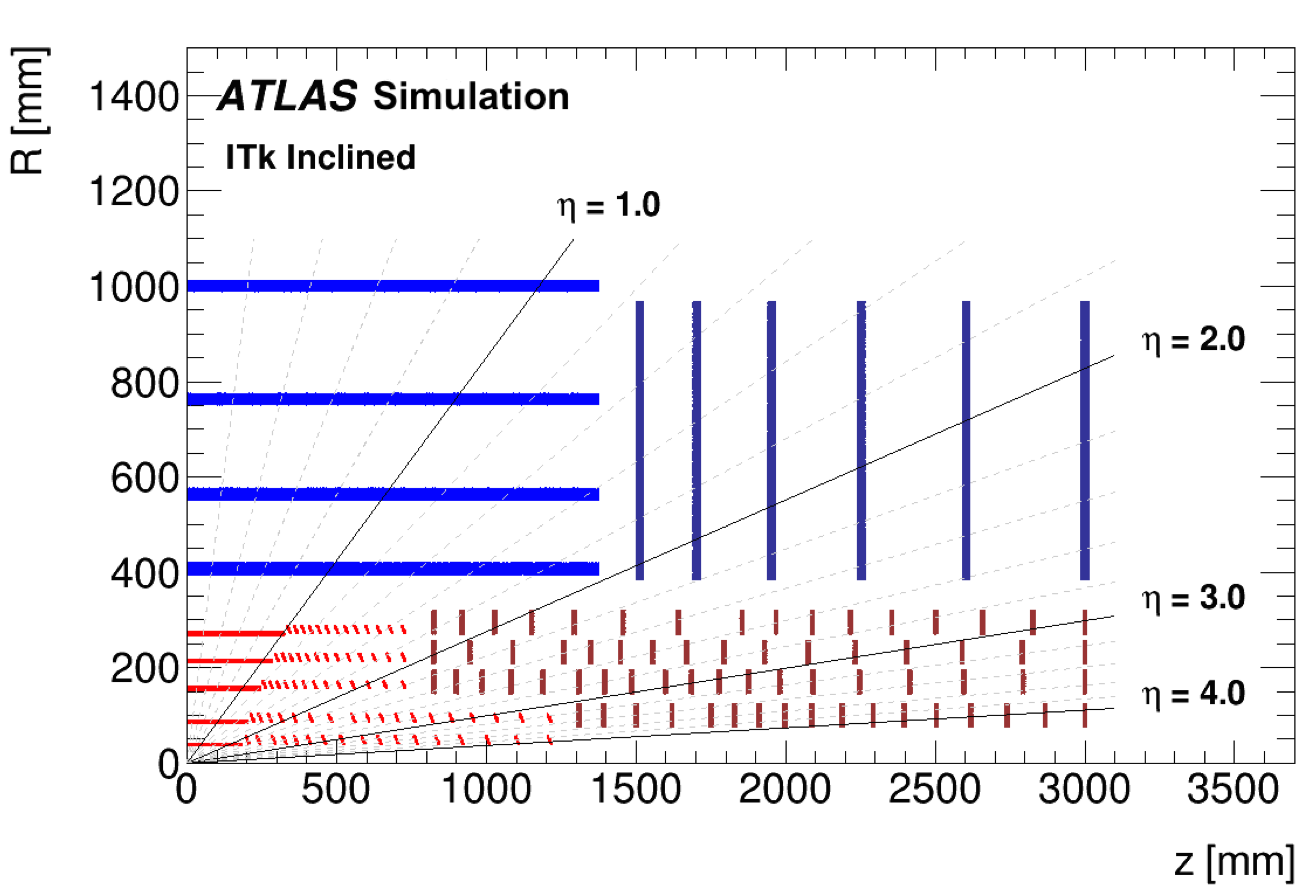
\includegraphics[height=8cm,keepaspectratio]{atlas_itk.png}
  \caption[ITkの断面図]{ITkの断面図 \cite{itk}。}
  \label{fig:itk-danmen}
\end{figure}

以上の理由により、ATLASの衝突点に最も近い検出器である内部飛跡検出器の総入れ替えを計画している。HL-LHCのために開発されている、新たな内部飛跡検出器を\textbf{ITk}(\textbf{I}nner \textbf{T}rac\textbf{k}er)と呼ぶ。
ITkの全体像を\fref{fig:hl-lhc-itk}に示す。ITkは全てシリコン半導体検出器から構成され、\fref{fig:itk-danmen}に示すように、TRTは廃止されて、内側にピクセル検出器、外側にストリップ検出器が配置されている。
%ピクセル検出器はバレル部の5層とエンドキャップ部の 層、ストリップ検出器はバレル部の4層とエンドキャップ部の6層から構成され、ITk全体で$|\eta|<4$の領域を覆うように配置されている。

上で挙げた、放射線損傷についての問題を解消するために、ピクセル検出器に新たな半導体センサーを導入する。特に、放射線の影響が大きくなるバレル部の最内層では高放射線耐性を持つ3Dセンサーを使用することが予定されている。ヒット占有率の問題については、センサーの厚みを薄くし、ピクセルサイズを現行ピクセルの$1/5$にすることにより、ヒット占有率を抑えることが期待される。さらに、1衝突あたりのパイルアップが高くなることから、読み出しシステムの高速化も必要となる。


このようなアップグレードを行うことにより、HL-LHCにおける高い瞬間ルミノシティ環境下においても、高い飛跡再構成効率における解析を行うことができる。
さらに、現行LHCの検出範囲外であった$2.7<|\eta|$が検出可能になることにより、フェイクレートを抑えつつ、$3\ \si{GeV}$以上のミューオンを$99\si{\%}$以上の効率で検出、さらには$1\ \si{GeV}$以上の電子やパイオンを$85\si{\%}$以上の効率で検出可能となる。



%----------------------------------------------------------------------------
\subsection{HL-LHC physics}
\label{sec:hl-lhc-physics}
%----------------------------------------------------------------------------

%素粒子のところと内容を合わせる。
%統計量がどれくらい必要で、それが再現できる?

%\fref{fig:hl-lhc}にある運転計画のように、LHCでは2010年の運転開始から統計をため、積分ルミノシティはRUN1の終了時において$30\ \si{fb^{-1}}$、RUN2の終了時において$190\ \si{fb^{-1}}$となっている。



\newpage

%----------------------------------------------------------------------------
\chapter{シリコンピクセル検出器}
\label{sec:}
%----------------------------------------------------------------------------






%----------------------------------------------------------------------------
\section{半導体検出器の一般論}
\label{sec:}
%----------------------------------------------------------------------------








%----------------------------------------------------------------------------
\section{ピクセル検出器}
\label{sec:}
%----------------------------------------------------------------------------











%----------------------------------------------------------------------------
\section{現行ピクセル検出器}
\label{sec:genkoupixel}
%----------------------------------------------------------------------------






%----------------------------------------------------------------------------
\section{新型ピクセル検出器}
%----------------------------------------------------------------------------





\newpage

%------------------------------------------------------------------------------------------------------------------------
\chapter{現行ピクセルモジュールの電荷較正}
\label{sec:chap3}
%------------------------------------------------------------------------------------------------------------------------

FEチップから得られるToT(Time over Threshold)を荷電粒子がシリコンセンサーに落とす電荷に較正する必要がある。本章では、電荷較正のための試験電荷生成回路の詳細について説明し、その後に電荷較正手法について述べる。

%------------------------------------------------------------------------------------------------------------------------
\section{試験電荷生成回路}
\label{sec:analog}
%------------------------------------------------------------------------------------------------------------------------
\fref{fig:analog}に試験電荷生成回路の概略図を示す。センサーにおいて生成された電子をFEチップにおいて検知するために、バンプにより接合されている。内部電位によりバンプに向かってドリフトした電子を検出し、バンプの接合部からFEチップへ送り、その信号をToTにデジタル変換し、後段のフレキシブル基板へ信号を送る。

一方で、Thresholdの測定や電荷較正のために用いる電荷はFEチップ内の回路で生成する。FEチップにおいて試験電荷を生成するために、電圧$V_\mathrm{cal}$を自由に設定できる回路と2つのキャパシタ$C_\mathrm{low}, C_\mathrm{high}$が搭載されている。試験電荷生成のために、$C_\mathrm{low}=8\ \si{fF}$のキャパシタを用いる場合と、$C_\mathrm{low}+C_\mathrm{high}=40\ \si{fF}$の合成キャパシタを用いる場合がある。$C_\mathrm{low}+C_\mathrm{high}$の合成キャパシタを用いる場合は生成した試験電荷から得られるToTが約$10\%$小さく出力されることがわかっている。そのため、Thresholdの測定や電荷較正を行う際には、$C_\mathrm{low}$のキャパシタを用いて試験電荷の生成を行う。

\begin{figure}[tbp]
  \centering
  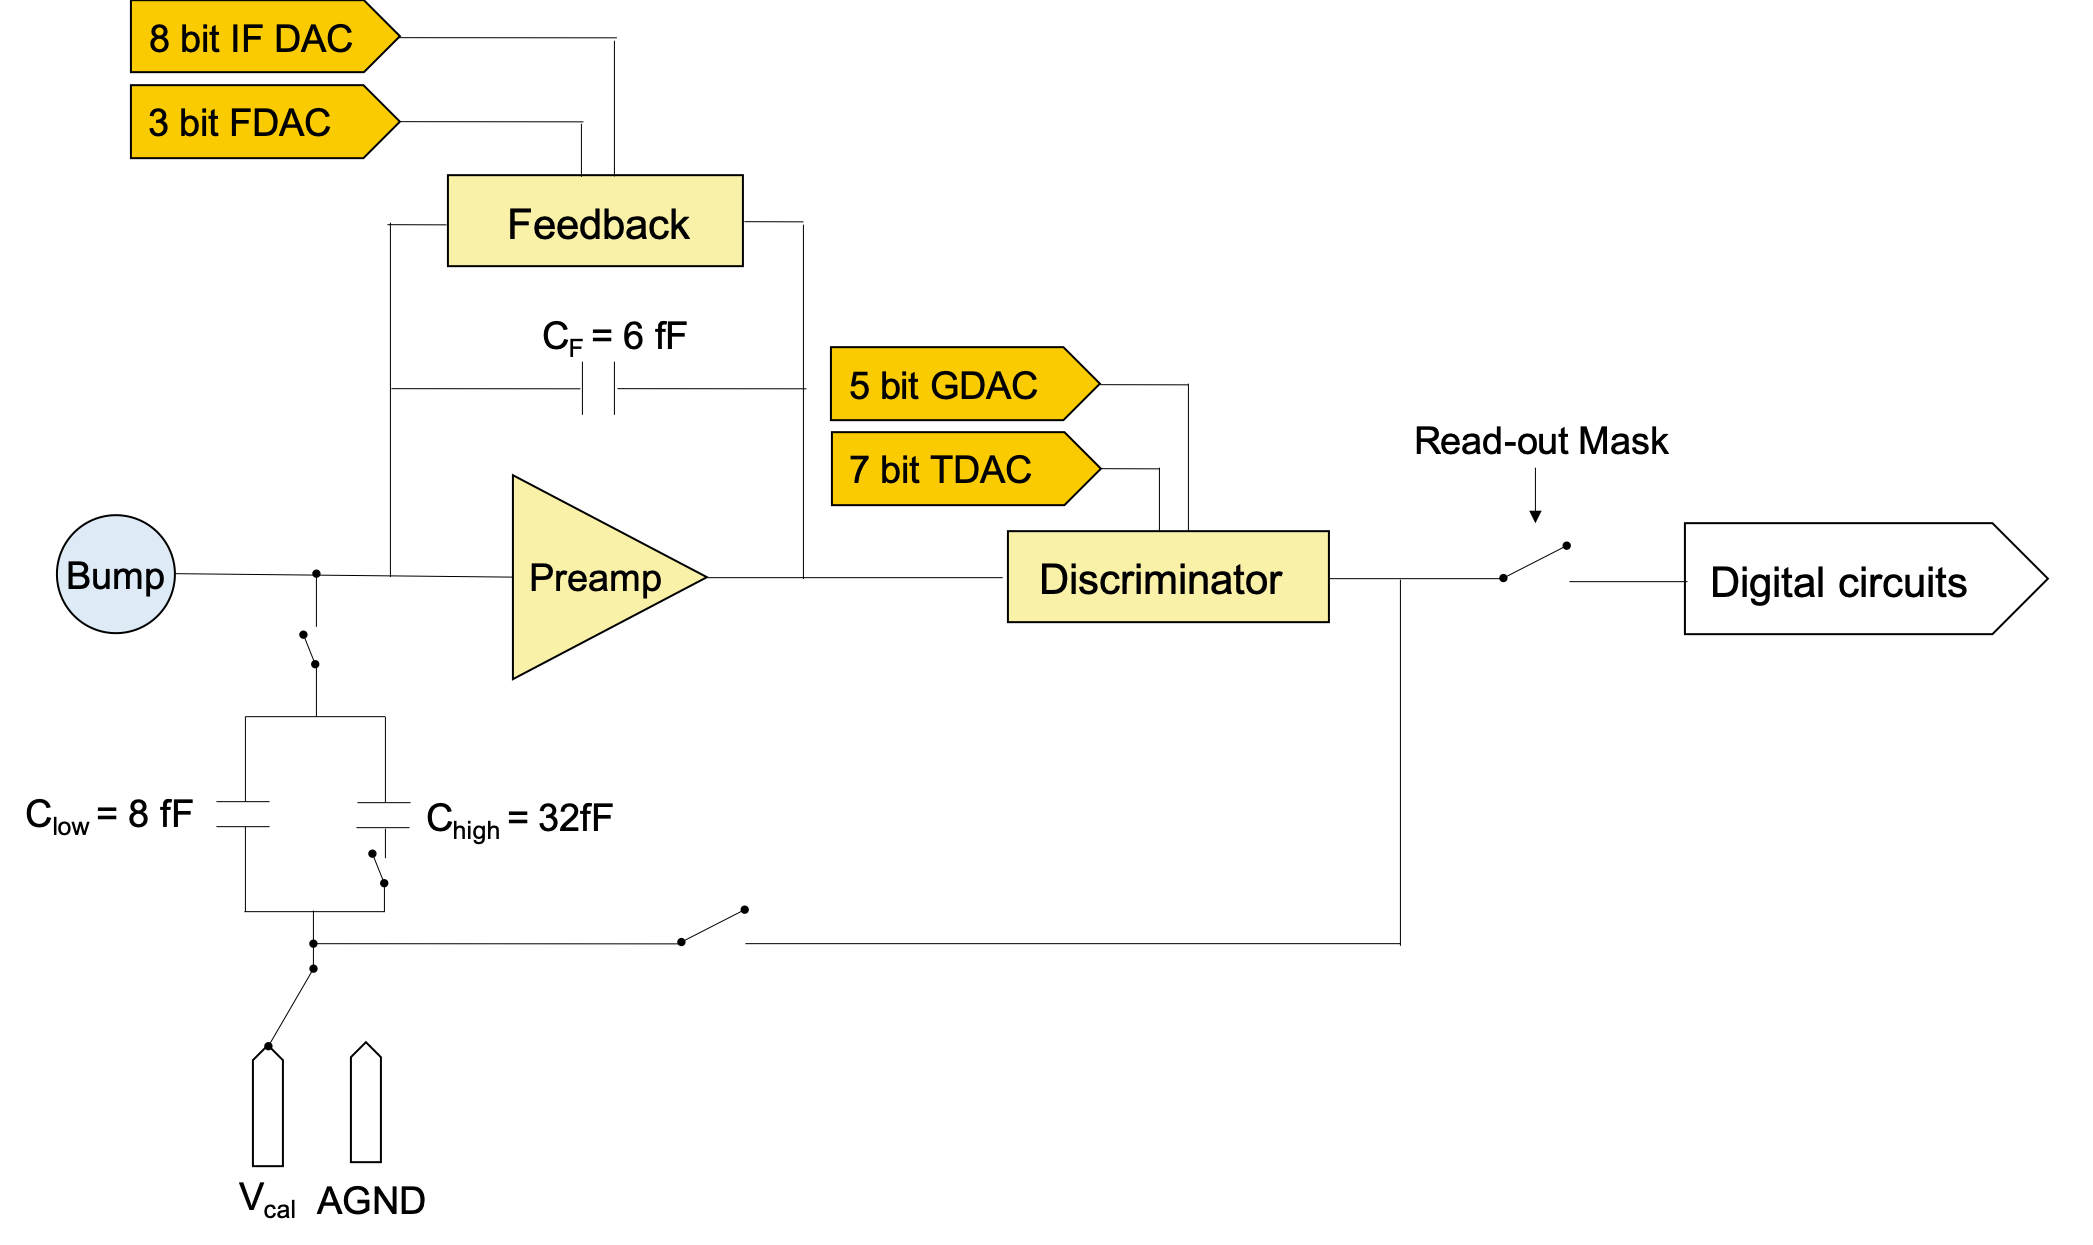
\includegraphics[height=7cm,keepaspectratio]{analog2.png}
  \caption[試験電荷生成回路の概略図]{試験電荷生成回路の概略図。電荷較正やThresholdスキャンのための試験電荷は$V_\mathrm{cal}$とキャパシタの組み合わせによって生成される。}
  \label{fig:analog}
\end{figure}


%------------------------------------------------------------------------------------------------------------------------
\section{電荷較正手法}
\label{sec:calibway}
%------------------------------------------------------------------------------------------------------------------------
ピクセルモジュールの出力であるToTを較正し、荷電粒子が落とした電荷量に変換する方法について説明する。各ピクセル間の差異を少なくするために、ToTの較正を行う前に、ThresholdやToTを目標値になるようチューニングを行う必要がある。以下ではチューニングと電荷較正の方法について説明する。


%------------------------------------------------------------------------------------------------------------------------
\subsection{チューニング}
\label{sec:tuning}
%------------------------------------------------------------------------------------------------------------------------
各ピクセルにおけるThresholdと、ある基準電荷量の信号に対するToTを任意の値に調整するためにFEチップのチューニングを行う。RUN2におけるThresholdおよび任意の値に対するToTの目標値をそれぞれ\tref{tab:thresholdtuning}、\tref{tab:tottuning}に示す。さらに、2022年3月から始まるRUN3では、B-LayerのThresholdは$3500\ \si{e}$でありToTのチューニングは$20\ \si{ke}$の電荷に対して$18\ \si{ToT}$、IBLのThresholdは$1500\ \si{e}$でありToTのチューニングは$16\ \si{ke}$の電荷に対して$10\ \si{ToT}$である。

\begin{table}[tbp]
  \begin{center}
    \caption[各LayerにおけるThresholdの値]{各LayerにおけるThresholdの目標値。}
    \label{tab:thresholdtuning}
    \begin{tabular}{|l||r|r|r|r|}
    \hline
      Layer名  & 2015年($4\ \si{fb^{-1}}$) & 2016年($39\ \si{fb^{-1}}$) & 2017年($50\ \si{fb^{-1}}$) & 2018年($63\ \si{fb^{-1}}$) \\
    \bhline{1.5pt}
      IBL & $2500$ & $2500$ & $2500$ & $2000$ \\
    \hline
      B-Layer(中央) & $3500$ & $3500$ & $5000$ & $4300$ \\
    \hline
      B-Layer(前方) & $3500$ & $3500$ & $5000$ & $5000$ \\
    \hline
      Layer1 & $3500$ & $3500$ & $3500$ & $3500$ \\
    \hline
      Layer2 & $3500$ & $3500$ & $3500$ & $3500$ \\
    \hline
      Disk & $3500$ & $3500$ & $4500$ & $3500$ \\
    \hline
    \end{tabular}
  \end{center}
\end{table}


\begin{table}[tbp]
  \begin{center}
    \caption[各LayerにおけるToTのチューニングの値]{各LayerにおけるToTの目標値。表中における括弧はToTに対する電荷量であり、この値はMIP粒子がセンサーに落とす電荷量を表す。}
    \label{tab:tottuning}
    \begin{tabular}{|l||r|r|r|r|}
    \hline
      Layer名  & 2015年($4\ \si{fb^{-1}}$) & 2016年($39\ \si{fb^{-1}}$) & 2017年($50\ \si{fb^{-1}}$) & 2018年($63\ \si{fb^{-1}}$) \\
    \bhline{1.5pt}
      IBL & $10 \mathrm{ToT} (16\ \si{ke})$ & $8 \mathrm{ToT} (16\ \si{ke})$ & $8 \mathrm{ToT} (16\ \si{ke})$ & $10 \mathrm{ToT} (16\ \si{ke})$ \\
    \hline
      B-Layer & $30 \mathrm{ToT} (20\ \si{ke})$ & $18 \mathrm{ToT} (20\ \si{ke})$ & $18 \mathrm{ToT} (20\ \si{ke})$ & $18 \mathrm{ToT} (20\ \si{ke})$ \\
    \hline
      Layer1 & $30 \mathrm{ToT} (20\ \si{ke})$ & $30 \mathrm{ToT} (20\ \si{ke})$ & $30 \mathrm{ToT} (20\ \si{ke})$ & $30 \mathrm{ToT} (20\ \si{ke})$ \\
    \hline
      Layer2 & $30 \mathrm{ToT} (20\ \si{ke})$ & $30 \mathrm{ToT} (20\ \si{ke})$ & $30 \mathrm{ToT} (20\ \si{ke})$ & $30 \mathrm{ToT} (20\ \si{ke})$ \\
    \hline
      Disk & $30 \mathrm{ToT} (20\ \si{ke})$ & $30 \mathrm{ToT} (20\ \si{ke})$ & $30 \mathrm{ToT} (20\ \si{ke})$ & $30 \mathrm{ToT} (20\ \si{ke})$ \\
    \hline
    \end{tabular}
  \end{center}
\end{table}

チューニングには、あるFEチップにおける全ピクセルのTresholdと任意の値に対するToTを調整するためのglobalチューニングと各ピクセルごとの値を目標値に近づけるlocalチューニングがある。はじめに、globalチューニングを行い、全ピクセルのThresholdまたはToTを大まかに目標値に合わせる。この段階では、全ピクセルから得られる分布の分散は大きいため、localチューニングを行い各ピクセルが返す値を目標値にさらに近づける。
%ToTの値はThresholdに依存するため、Thresholdのチューニングの前後においてToTが変わってしまう。また、同様にToTチューニングの後はThreshold値が変化してしまう。この影響は、チューニングを繰り返すことで小さくなり、

チューニングの後、ThresholdスキャンやToTスキャンを行い各ピクセルにおける値を測定する。ThresholdスキャンおよびToTスキャンの方法を以下に述べる。

%------------------------------------------------------------------------------------------------------------------------
\subsubsection{Thresholdスキャン}
\label{sec:thresholdscan}
%------------------------------------------------------------------------------------------------------------------------
Thresholdスキャンでは、各ピクセルに試験電荷を入射しThresholdとノイズを測定する。試験電荷を増加させつつ検出効率を測定し、\fref{fig:threshold}に示す様な分布を作成する。この分布はS字を描くため、\textbf{Sカーブ}と呼ばれている。\fref{fig:threshold}中の青線はSカーブのフィッティングであり、\eref{eq:gosakannsuu}のような誤差関数を用いて定義される。
\begin{equation}
  \label{eq:gosakannsuu}
  f(x)=0.5\times\left[ 2-\mathrm{erfc}\left( \frac{x-Q_\mathrm{threshold}}{\sigma \times \sqrt{2}} \right)  \right] \times p
\end{equation}
Sカーブにおいて、検出効率が$50\%$となる試験電荷の値をThresholdと定義し、検出効率が$30\%$と$70\%$となる試験電荷の幅をノイズと定義する。

\begin{figure}[tbp]
  \centering
  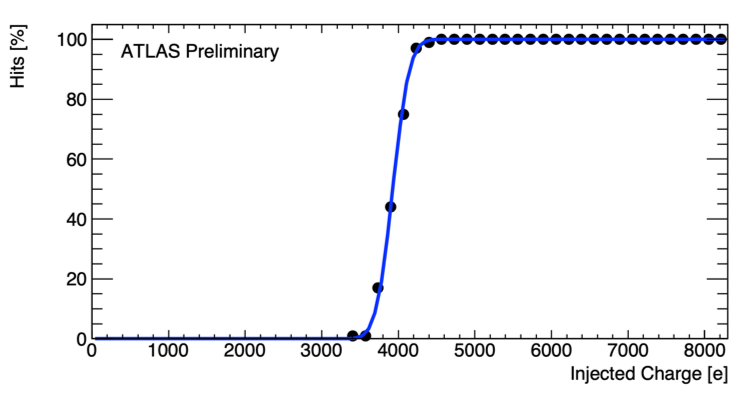
\includegraphics[height=7cm,keepaspectratio]{threshold.png}
  \caption[検出効率と試験電荷の関係]{検出効率と試験電荷の関係 \cite{calibsoft}。検出効率が 50\% となる試験電荷の値がThresholdであり、検出効率が30\%と 70\% となる試験電荷の幅がノイズである。}
  \label{fig:threshold}
\end{figure}


%------------------------------------------------------------------------------------------------------------------------
\subsubsection{ToTスキャン}
\label{sec:totscan}
%------------------------------------------------------------------------------------------------------------------------
ToTスキャンでは、一定の試験電荷を各ピクセルに100回入射させ、その試験電荷に対するToTの値の測定を行う。各ピクセルから得られるToTの値はデジタル値であるため整数値であるが、100回のスキャンの平均値をある試験電荷に対するToTとするため、この値は小数値を取り得る。


%------------------------------------------------------------------------------------------------------------------------
\subsection{電荷較正}
\label{sec:calibration}
%------------------------------------------------------------------------------------------------------------------------
\ref{sec:ASIC}で示した様に、ToTは荷電粒子がシリコンセンサーに落とす電荷量$Q$に比例すると予想される。しかし、実際には三角波の傾きが完全に一致しないこと等による二次な効果により、ToTと電荷量は直線ではなくなり\eref{eq:calibration}の様に表される。
\begin{equation}
  \label{eq:calibration}
  \mathrm{ToT} = p_0\frac{p_1 + Q}{p_2 + Q}
\end{equation}
\eref{eq:calibration}に示した3つのパラメータを求めるために、電荷量を変えながら試験電荷を入射し、ToTの較正を行う。電荷較正は各ピクセルに対してパラメータを求めるのではなく、FEチップごとに一律の値を用いる。そのため、ToTスキャンから得られたピクセルごとのToTの平均値を用いてFEチップに対する電荷較正を行う。

IBLについてはToTの出力が4bitと少ないことから、RUN3からは\eref{eq:calibration}によるフィッティングは行わず、ToTの値と試験電荷の値をルックアップテーブルを用いて変換を行う。本研究では電荷較正手法について取り扱うため、以下ではピクセル検出器についてのみについて述べる。

%------------------------------------------------------------------------------------------------------------------------
\section{電荷較正結果の履歴}
\label{sec:probrem}
%------------------------------------------------------------------------------------------------------------------------
Thresholdのチューニングや電荷較正を行った後、それらに関する情報はCERNに設置されているデータベース\cite{pixeldb}に保存する必要がある。このデータベースでは電荷較正に関する情報や検出器の配置や温度等のDCS(Data Control System)情報、さらにトリガー情報等を保管する。これらの情報は、測定におけるイベント選別やモンテカルロシミュレーションのためのイベント作成等に用いられる。

ThresholdスキャンおよびToTスキャンは各ピクセルごとの値を出力するが、データベースへはあるFEチップにおけるThresholdの平均値およびToTの平均値を用いた電荷較正式(\ref{eq:calibration})のパラメータのみを登録する。また、各ピクセルの大部分は\tref{tab:asicsiyou}に示した構造をしているが、FEチップの境界付近では不感領域をなるべく少なくするために、構造の異なったピクセルを配置する。FE-I3の境界付近におけるピクセルの構造を\fref{fig:pixeltypes}に示す。\tref{tab:asicsiyou}に示した通常のピクセルのことをnormalピクセル(図中の青の領域)と呼び、黄色の領域のピクセルをlongピクセル、赤色の領域をgangedピクセルと呼ぶ。longピクセルは$50\times 600\ \si{\micro m^2}$であり、長方形の一辺の長さがnormalピクセルの1.5倍となっている。また、gangedピクセルはnormalピクセル2つをワイヤーで接続した構造をしている。このような構造の違いから、ノイズ等の値が異なる値になるため、データベースへはそれぞれの値をアップロードする。

\begin{figure}[tbp]
  \centering
  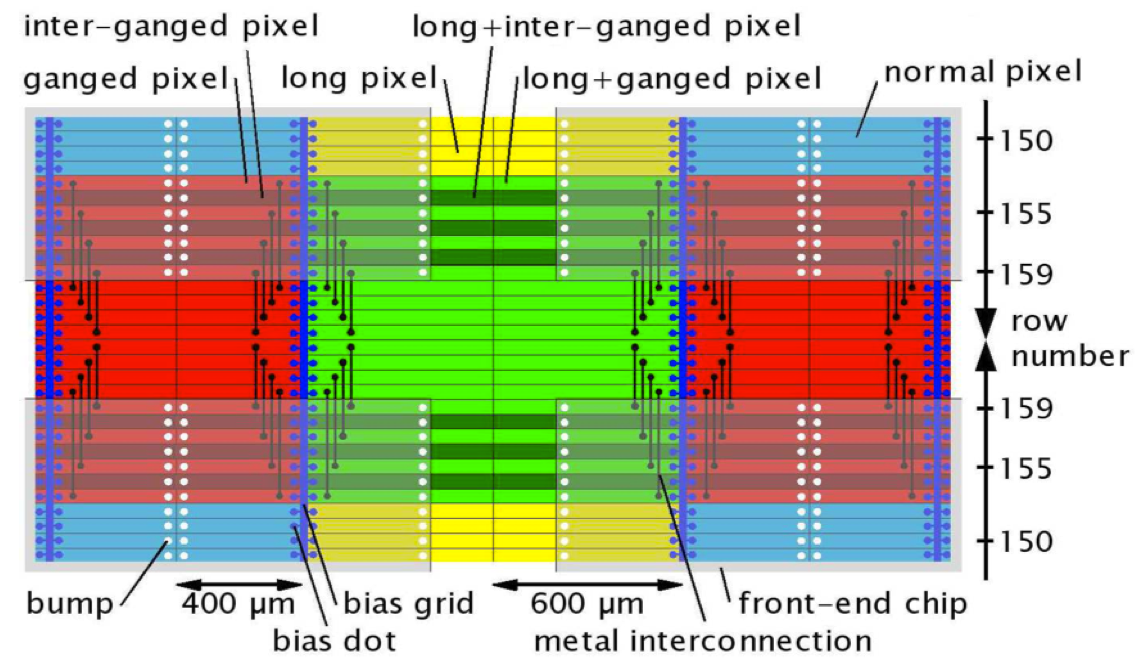
\includegraphics[height=6cm,keepaspectratio]{pixeltypes2.png}
  \caption[ピクセルモジュールのFEチップ境界付近のピクセルタイプ]{ピクセルモジュールのFEチップ境界付近のピクセルタイプ \cite{pixeltypes}。}
  \label{fig:pixeltypes}
\end{figure}

データベースに登録する情報を以下に示す。
\begin{itemize}
  \item Thresholdの平均値
  \item Thresholdの分散
  \item Thresholdのノイズ
  \item In-time threshold
  \item 電荷較正式(\ref{eq:calibration})における3つのパラメータ
  \item 電荷較正におけるフィッティングの誤差
\end{itemize}




\newpage

%------------------------------------------------------------------------------------------------------------------------
\chapter{電荷補正の最適化}
\label{sec:chap4}
%------------------------------------------------------------------------------------------------------------------------
Thresholdのチューニングおよび電荷較正を行った後、それぞれのパラメータが適切な値を保持していることを確認しデータベースに必要なパラメータ情報の登録を行う。ピクセルモジュールの電荷較正では正しく結果を出力しない場合があるため、電荷較正結果に適切な値を補完しデータベースにアップロードする必要がある。電荷較正の際に発生するいくつかの問題に対し、例外処理を行いより適切な値に近い値を補完するアルゴリズムの開発を行った。
本章では、電荷較正で発生する問題と、その問題に対する処理方法について説明する。

%------------------------------------------------------------------------------------------------------------------------
\section{電荷較正における補正の概要}
\label{sec:hoseigaiyou}
%------------------------------------------------------------------------------------------------------------------------

電荷較正では、ピクセル検出器およびIBLに搭載された計28400個のFEチップを同時に操作するため、全てが正常に機能しないことがある。電荷較正における問題は主に以下の2つがあげられる。
%本節ではそれぞれについての問題の原因とこれまでの補完方法について説明する。

\begin{itemize}
  \item[1. ] 不適当な電荷を使った電荷較正
  \item[2. ] データの欠陥
\end{itemize}

1つ目の問題に関して、ピクセルモジュールの電荷較正ではFEチップに搭載された回路を用いて試験電荷を生成し、ThresholdスキャンやToTスキャンを行う。電荷生成のための回路のいずれかの部分に故障等の問題があると、誤った試験電荷を生成してしまう。問題がある場合とない場合の試験電荷について、電荷較正\eref{eq:calibration}を用いてフィッティングした結果を\fref{fig:calibhikaku}に示す。\fref{fig:calibhikaku}において、左図は理想的なフィッティング結果を表しており、全ての点がフィット曲線上に乗っていることがわかる。この様に、ToTとセンサーが落とす電荷量は、おおよそ線形関係にあることがわかる。

\begin{figure}[tbp]
  \begin{minipage}[b]{0.5\linewidth}
    \centering
    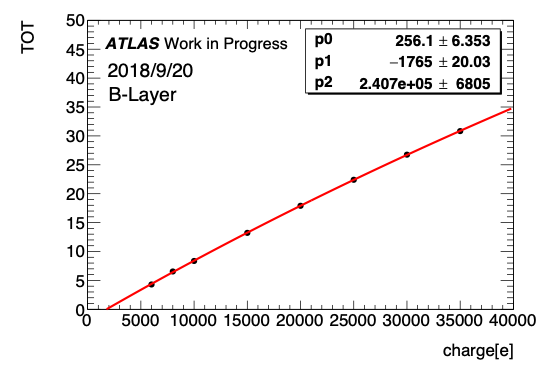
\includegraphics[keepaspectratio, scale=0.8]{goodcalib.png}
  \end{minipage}
  \begin{minipage}[b]{0.5\linewidth}
    \centering
    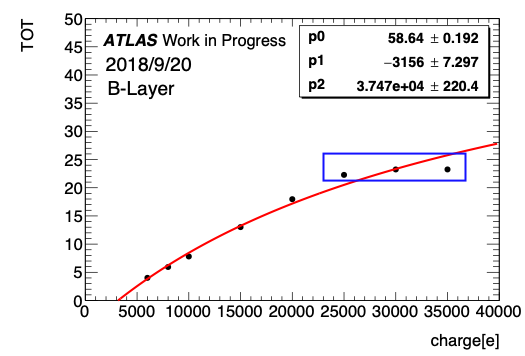
\includegraphics[keepaspectratio, scale=0.8]{badcalib.png}
  \end{minipage}
  \caption[電荷較正\eref{eq:calibration}を用いてフィッティングした結果]{電荷較正\eref{eq:calibration}を用いてフィッティングした結果。左図は理想的なフィッティング結果を表しており、右図は正しいToTが得られていない点を含むフィッティング結果である。}
  \label{fig:calibhikaku}
\end{figure}

一方で、右図は電荷生成の回路に問題のあるFEチップにおける電荷較正結果であり、電荷量の大きい3つの試験電荷についてToTの値がほとんど同じ値になっている。この原因は、試験電荷生成のための回路における電圧$V_\mathrm{cal}$の値が正しくキャパシタに渡されないことにある。$V_\mathrm{cal}$は\textbf{Plsr DAC}と呼ばれる$10\ \si{bit}$の値により決定される。$V_\mathrm{cal}$と$\mathrm{Plsr\ DAC}$の関係は\eref{eq:vcal}のように、1次式で与えられる。
\begin{equation}
  \label{eq:vcal}
  V_\mathrm{cal} = a + b\ (\mathrm{Plsr\ DAC})\ [\si{mV}]
\end{equation}
ここで、$a,\ b$は較正によって決定される定数であり、FEチップごとに個体差がある。あるFEチップに対する$V_\mathrm{cal}$とPlsr DACの関係の測定結果を\fref{fig:vcalplot}に示す。この図において、$\mathrm{Plsr\ DAC}\approx 750$までは$V_\mathrm{cal}$とPlsr DACの値が線形となっているが、それ以降のPlsr DAC値においては$V_\mathrm{cal}$が飽和していることがわかる。この$V_\mathrm{cal}$の飽和は、試験電荷生成回路におけるキャパシタ$C_\mathrm{low}$および$C_\mathrm{high}$の内、$C_\mathrm{low}$のみを用いて試験電荷を生成した場合に発生しやすいことがわかっている \cite{houwa}。\fref{fig:analog}に示したように、$C_\mathrm{high}$の前に配置されているスイッチを用いる事により使用するキャパシタの選択を行うことができる。電荷較正の際には、$C_\mathrm{low}$のみを用いるためこのスイッチは開放されているが、$V_\mathrm{cal}$の値が大きいときにはグランドへのリーク電流が大きくなってしまう。そのため、ある値以上の電荷を持つ試験電荷を正確に取得することができず、正しい電荷較正結果が得られない。$V_\mathrm{cal}$の飽和が起きていると予想される\fref{fig:calibhikaku}の右図の場合は、電荷較正に使用された試験電荷の内、正しいToTが得られていない2点を取り除き、再較正を行う必要がある。
\begin{figure}[tbp]
  \centering
  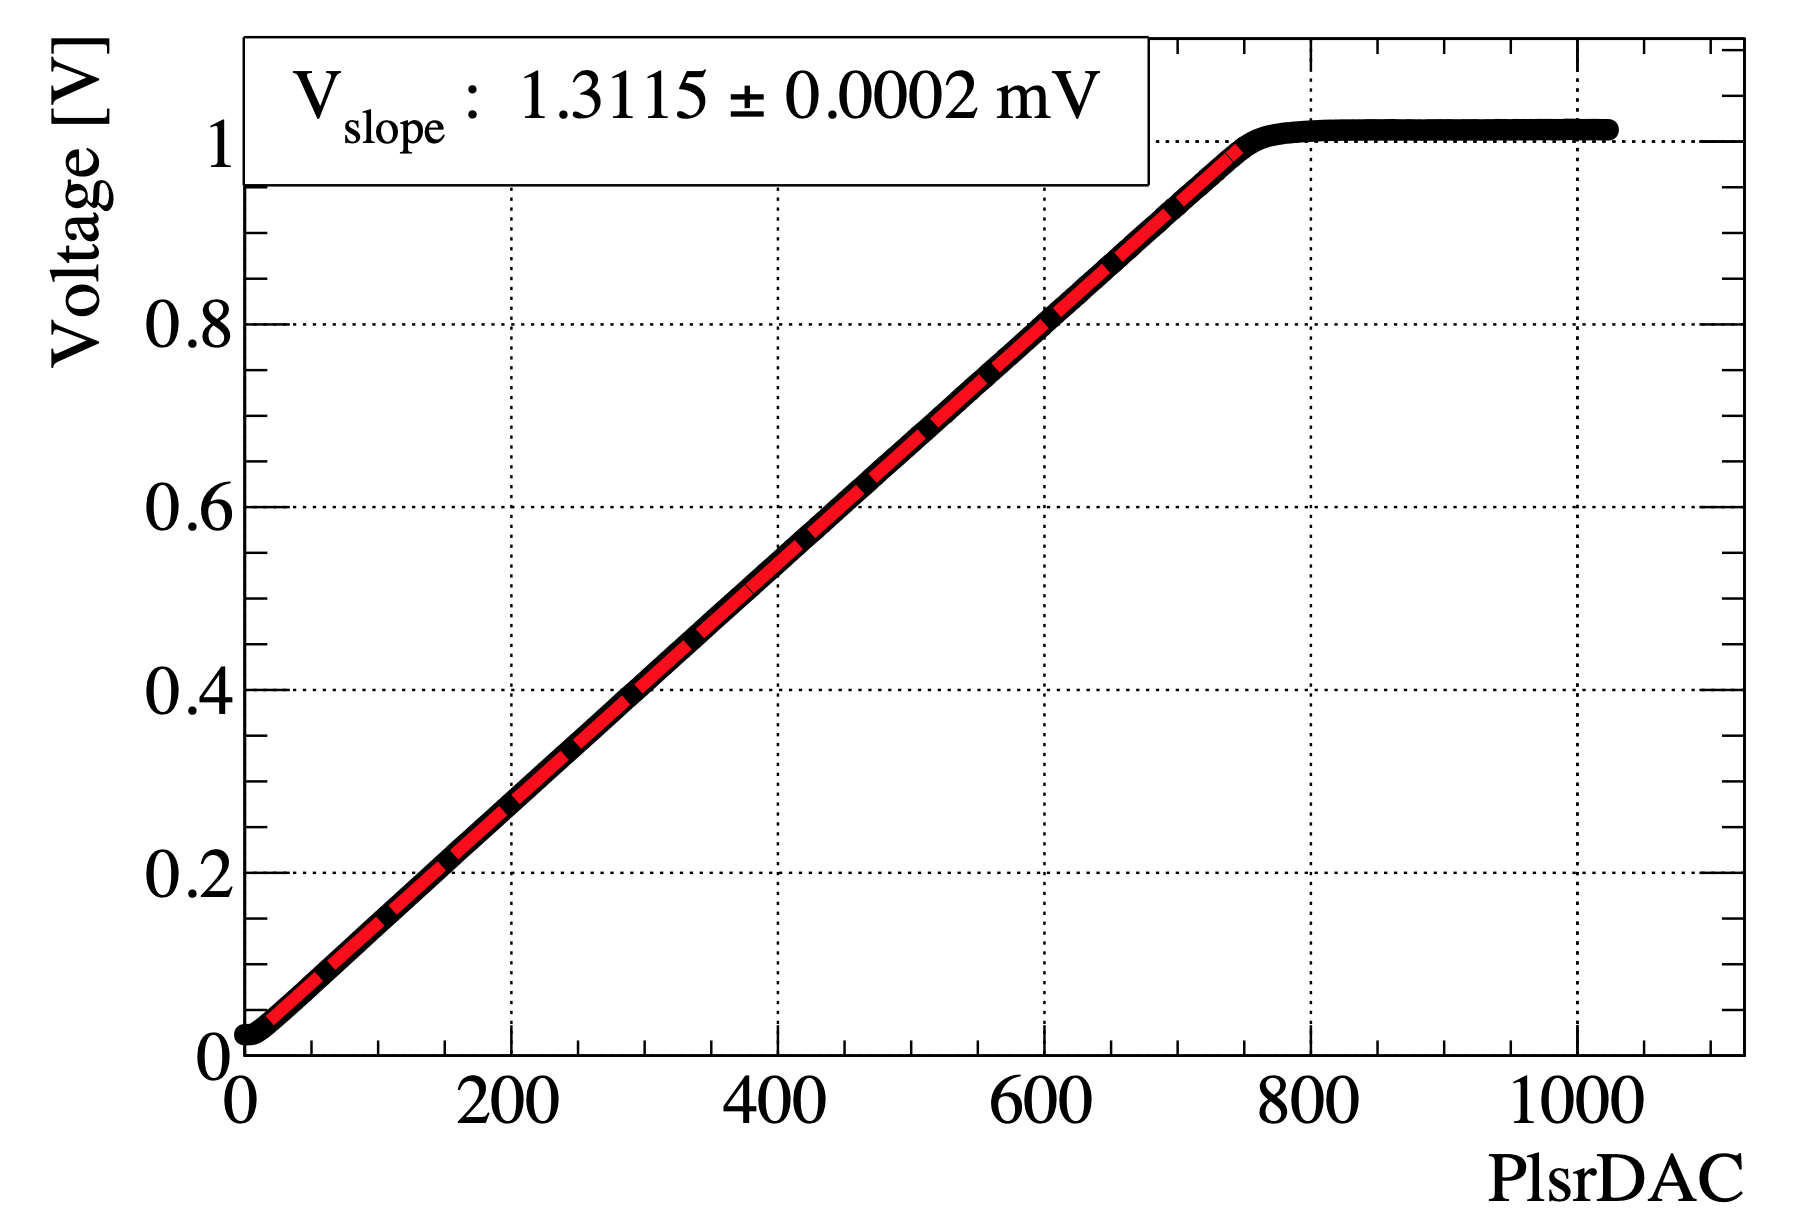
\includegraphics[height=7cm,keepaspectratio]{vcalplsr.png}
  \caption[$V_\mathrm{cal}$とPlsr DACの関係の測定結果]{$V_\mathrm{cal}$とPlsr DACの関係の測定結果 \cite{vcal}。黒点は各Plsr DACに対する$V_\mathrm{cal}$の測定点を表し、赤線は\eref{eq:vcal}を用いたフィッティング結果である。図中における$V_\mathrm{slope}$は赤線の傾きであり、\eref{eq:vcal}における$b$に対応する。}
  \label{fig:vcalplot}
\end{figure}

2つ目の問題に関して、あるFEチップに対してスキャンが失敗してしまった時にデータが欠陥してしまうことがある。例えば、Sカーブを用いてThresholdの値を計算するアルゴリズムについて、Sカーブのフィッティングが失敗した際にはThresholdの値がデフォルトで\textbf{0}が出力されるようになっている。そのため、あるFEチップ上の全てのピクセルでSカーブのフィッティングが失敗しているような場合はデータを失い、\fref{fig:thresholdkekkan}のI6が示す領域のようにFEチップ上の全てのピクセルにおいてThresholdの値は$0$を出力する。
このように、あるFEチップについて全てのデータが欠陥してしまっている場合には、他の電荷較正結果をコピーすることにより補完を行う。あるピクセルモジュールにおいてFEチップの一部の結果が欠陥してしまっている場合は最も近いFEチップから値をコピーすることにより補完を行う。\fref{fig:thresholdkekkan}のようにあるモジュール上の一部のFEチップみにデータの欠陥が見つかった場合は、最も近いFEチップ(\fref{fig:thresholdkekkan}の場合はI5、I7、I9のいずれか1つ)から値をコピーすることによって補完作業を行う。一方で、あるモジュールについて全てのFEチップの結果が欠陥している場合は、直前に行われた電荷較正結果をコピーすることにより補完を行う。

\begin{figure}[tbp]
  \centering
  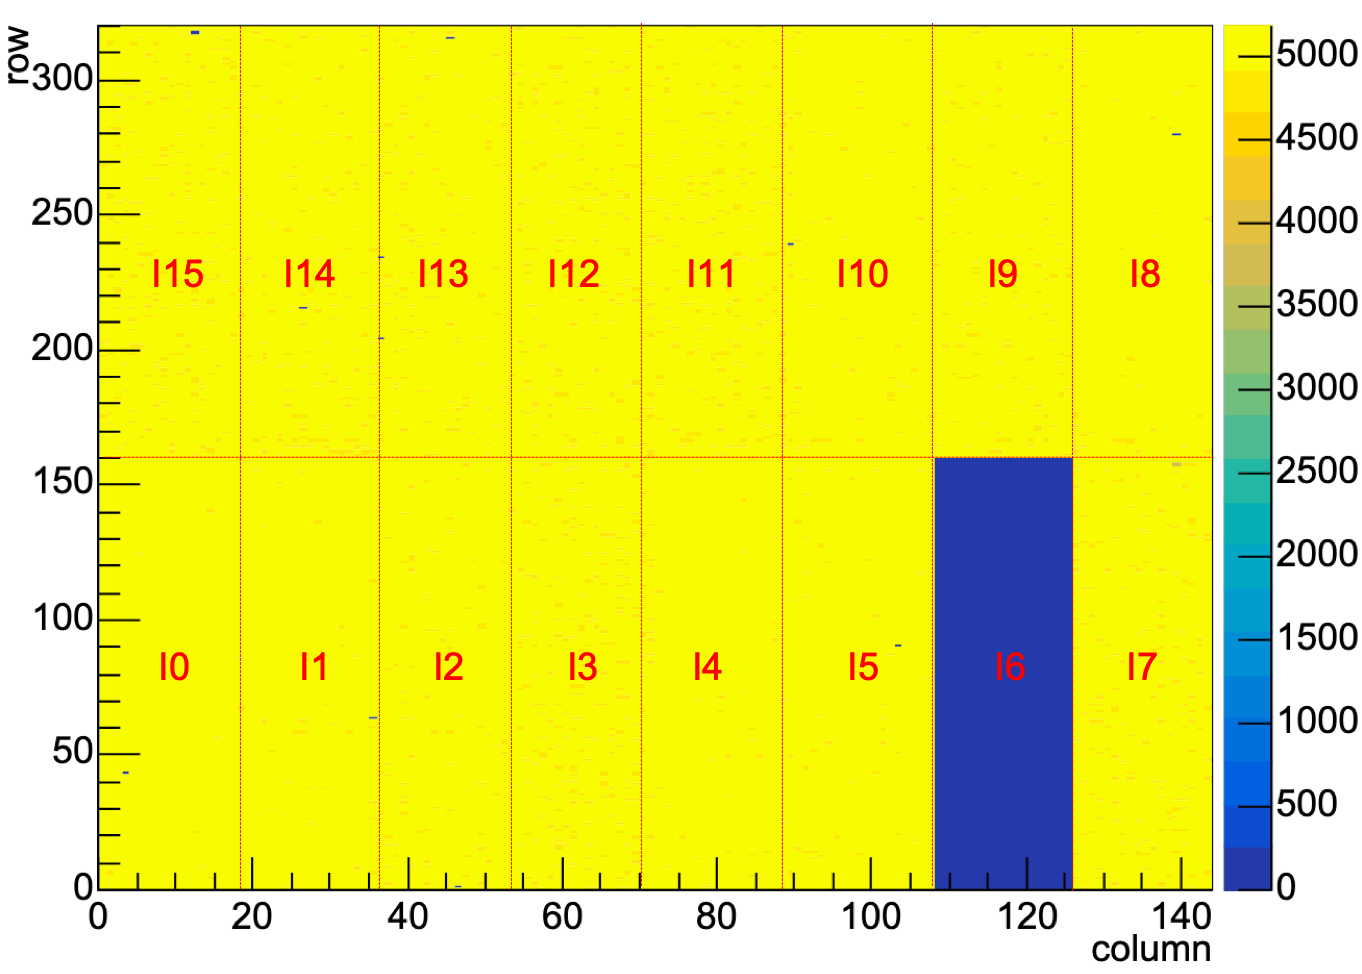
\includegraphics[height=7cm,keepaspectratio]{thresholdkekkan.png}
  \caption[欠陥が含まれるピクセルモジュールについてのThreshold分布]{欠陥が含まれるピクセルモジュールについてのThreshold分布。赤色の点線は$2\times8$ [行$\times$列]上に配置されたFE-I3の境界部分を表す。この図のように、ThresholdスキャンやToTスキャンの結果はモジュールごとに出力され、行と列の領域を指定することによりFEチップの識別を行うことができる。}
  \label{fig:thresholdkekkan}
\end{figure}

%------------------------------------------------------------------------------------------------------------------------
\subsection{これまでの電荷較正の再補正}
\label{sec:prehosei}
%------------------------------------------------------------------------------------------------------------------------

ATLASに搭載されたピクセル検出器およびIBLのピクセルモジュールについて電荷較正を行うが、測定を行っていると放射線損傷の影響によって、補正値がずれてしまう。\fref{fig:thresholdhennka}にRUN2におけるIBLのMIP粒子に対するToTの推移を示す。
このToTの推移はトータルドーズ効果による放射線損傷(\fref{fig:totaldoze}参照)を受けることによるものである。
放射線損傷が小さい場合(TID $\leq1\ [\si{Mrad}]$)、FEチップ電流は増加する。そのため、実行的なThreshold値が大きくなり、MIP粒子に対するToTは小さくなる(\fref{fig:thresholdhennka}の上図)。
一方で、放射線損傷が大きい場合(TID $\geq1\ [\si{Mrad}]$)、FEチップ電流は小さくなる。そのため、実行的なThreshold値が小さくなり、ToTの値は大きくなる(\fref{fig:thresholdhennka}の下図)。

%トータルドーズ効果とセンサーの漏れ電流の関係を\fref{fig:totaldoze}示す。

%IBLではMIP粒子がセンサーに落とす電荷量は$16\ \si{ke}$であるが、
このように、放射線損傷を受けることによりToTの値が目標値である$10\ \si{ToT}$から変化していることがわかる。目標値から大きくずれてしまうと、検出器を通過する荷電粒子がセンサーに落とす電荷量を正確に測定できなくなり、位置分解能が悪くなる。さらに、ThresholdやToTの分散も大きくなることから、信号とノイズの分離が悪くなる可能性がある。
目標値からのずれを補正するため、2018年における電荷較正は2週間から4週間の周期で行い、電荷較正の後には\ref{sec:hoseigaiyou}節で説明した問題を取り除くため、補完作業を行う必要がある。

\begin{figure}[tbp]
  \centering
  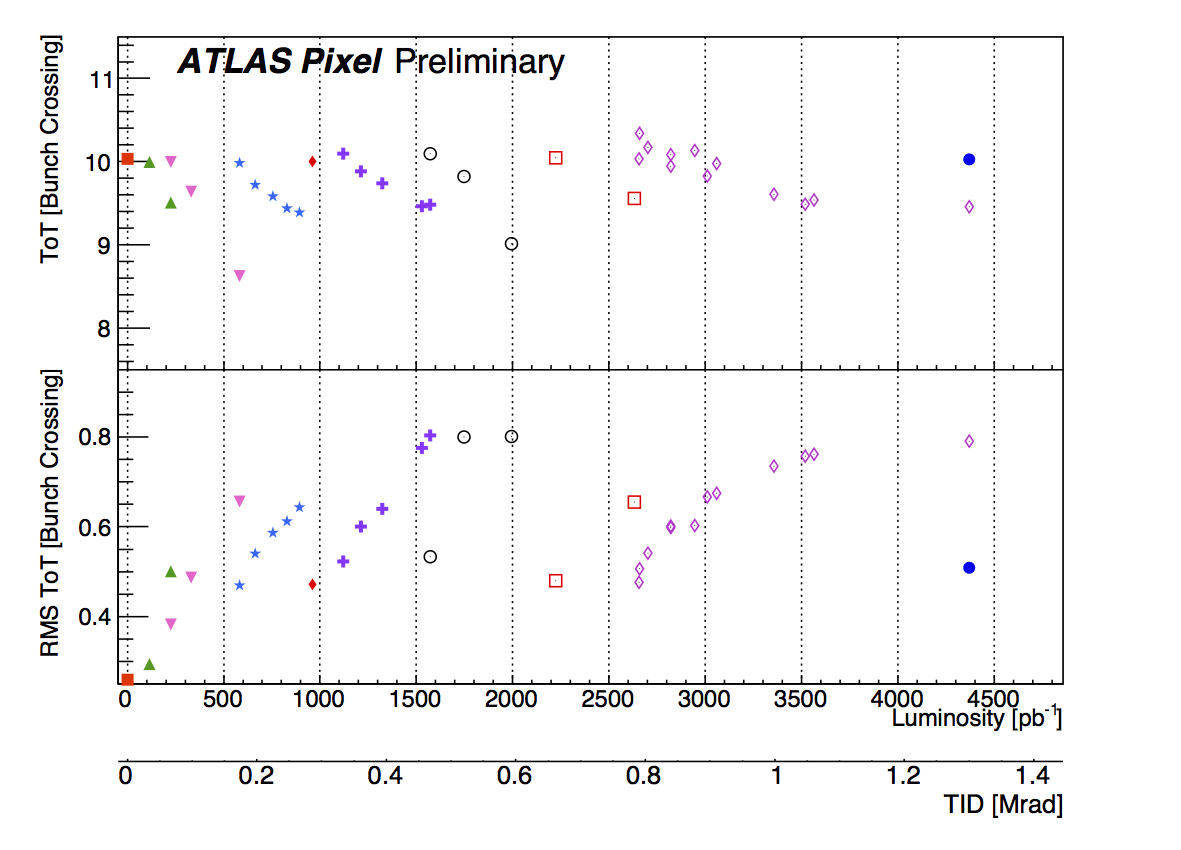
\includegraphics[height=7.8cm,keepaspectratio]{tothennkarow.png}
  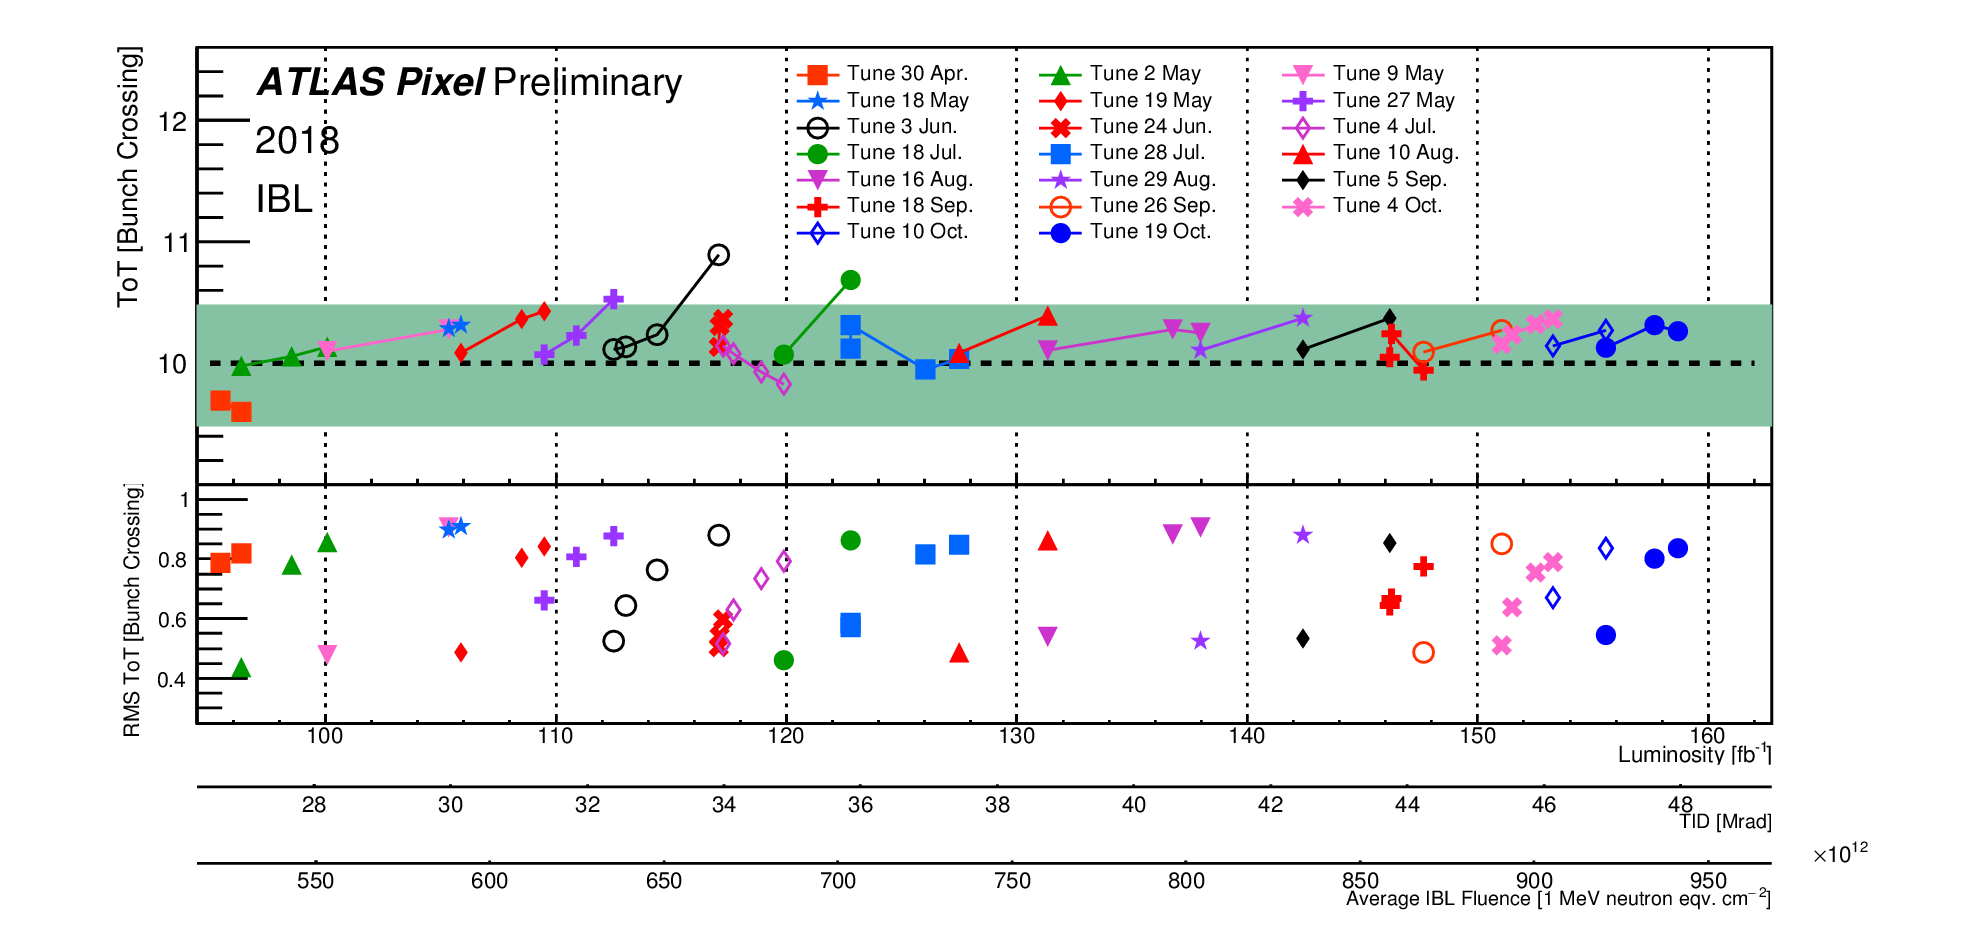
\includegraphics[height=7.5cm,keepaspectratio]{tothennka.png}
  \caption[ルミノシティに対するToTの変化]{IBLのルミノシティに対するToTの変化 。各マーカーの左端は電荷較正直後のToTスキャン結果であり、電荷較正を行う事により放射線損傷によるずれが補正されている様子がわかる。上図は2015年におけるToTの変化\cite{tothenkarow}であり、左端はRun2開始時を表す。下図は2018年におけるToTの変化\cite{tothennka}で右端はRun2の最後を表す。IBLのToTの目標値は$16\ \si{ke}$の電荷量に対して$10\ \si{ToT}$であるが、トータルドーズ効果の影響を受け目標値からずれてしまう。}
  \label{fig:thresholdhennka}
\end{figure}


%\begin{figure}[tbp]
%  \begin{minipage}[b]{0.5\linewidth}
%    \centering
%    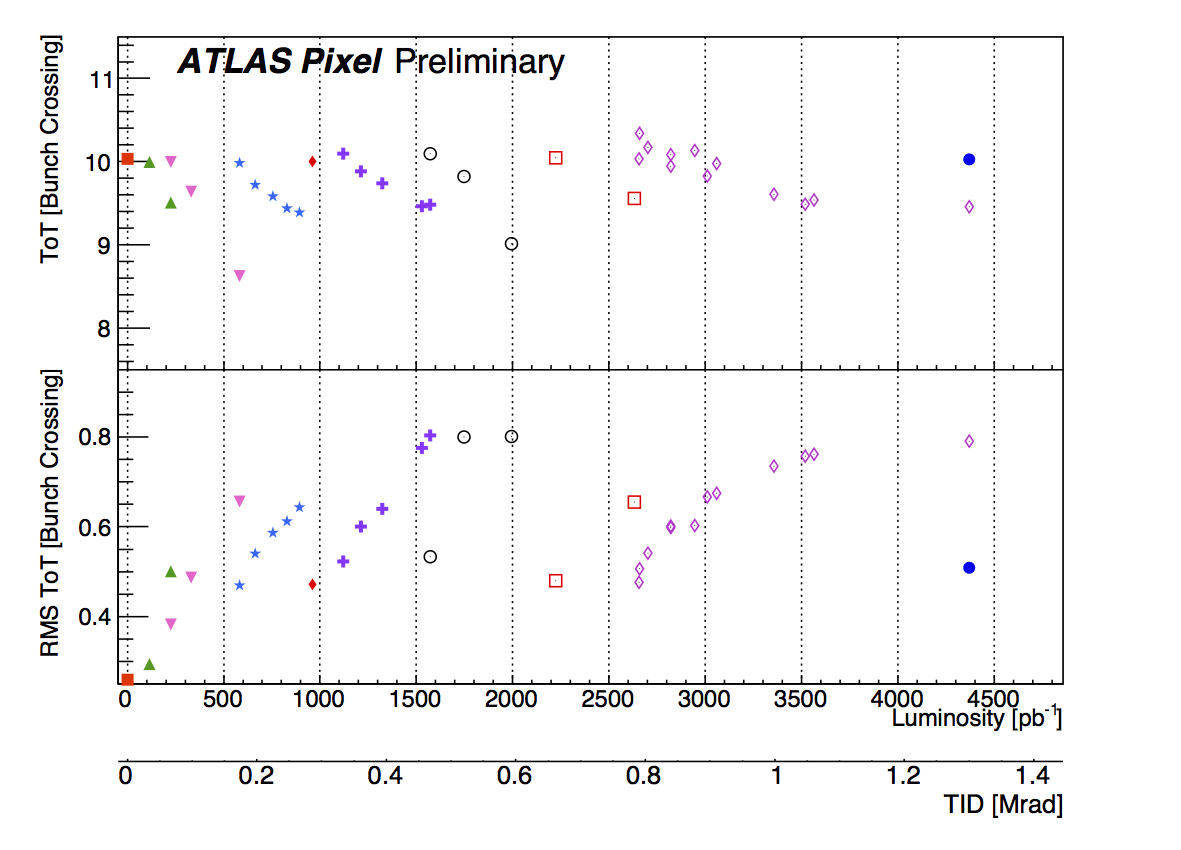
\includegraphics[keepaspectratio, scale=0.4]{tothennkarow.png}
%  \end{minipage}
%  \begin{minipage}[b]{0.5\linewidth}
%    \centering
%    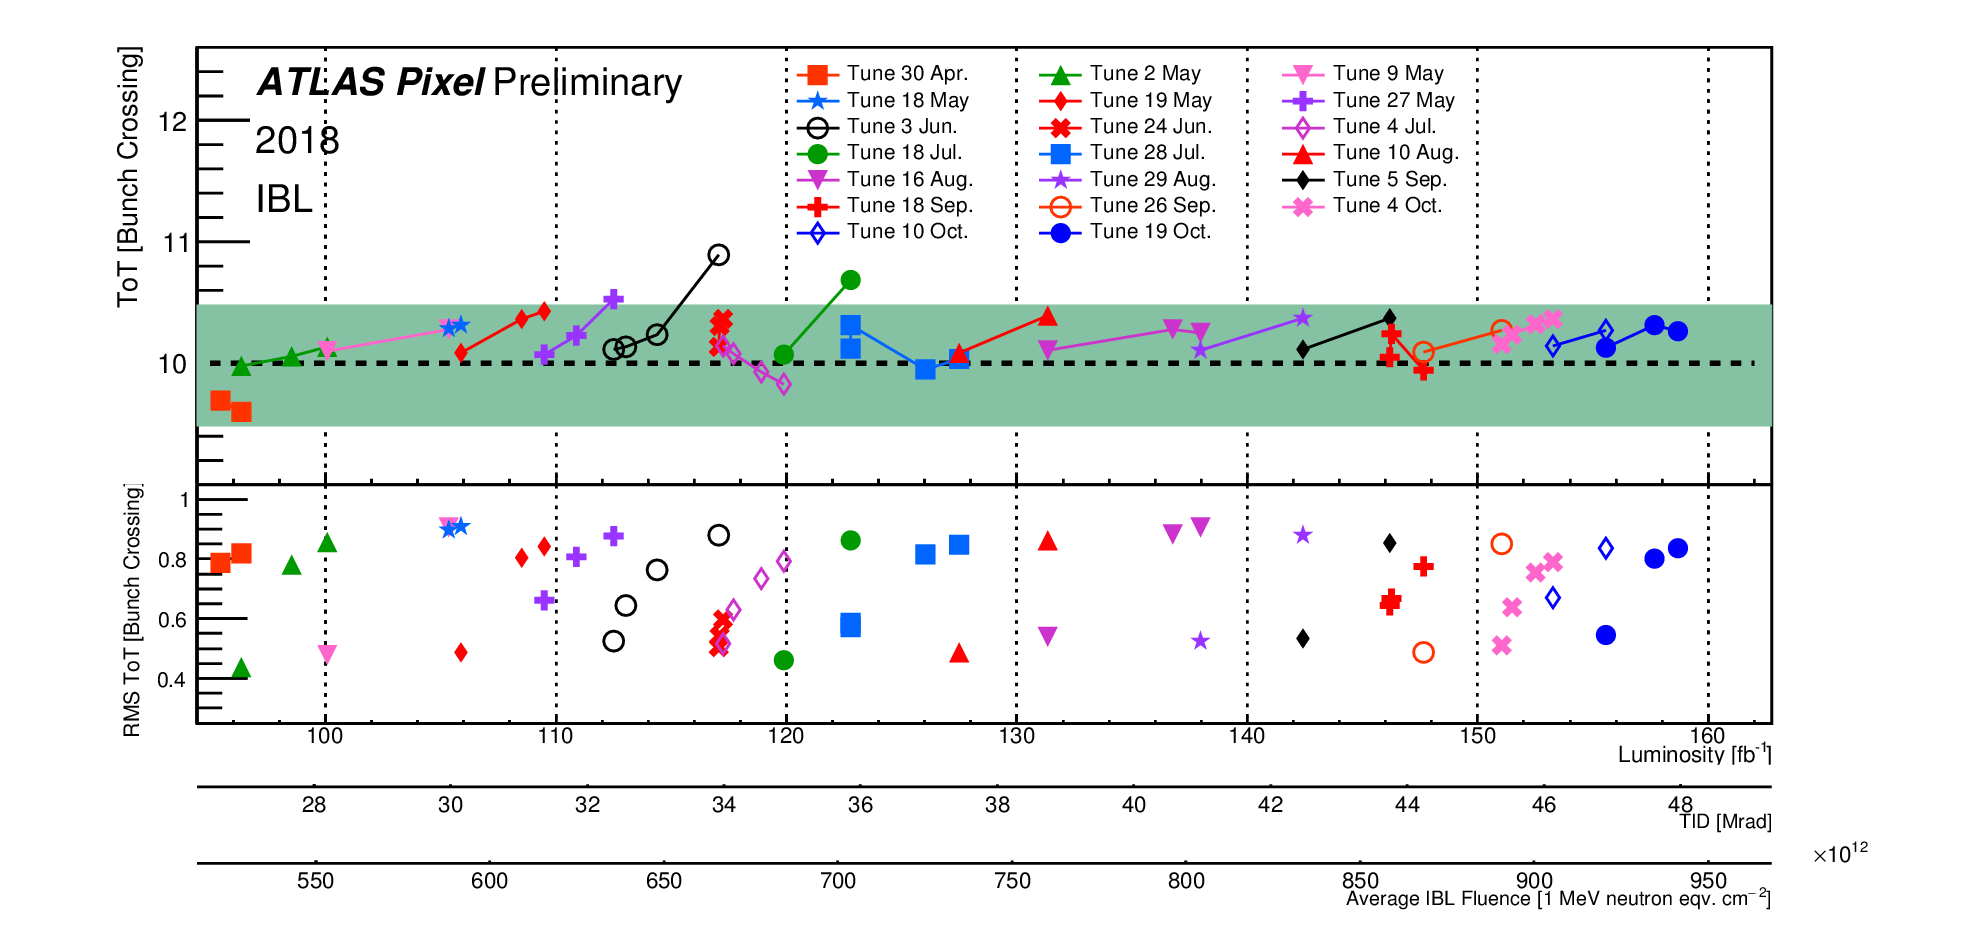
\includegraphics[keepaspectratio, scale=0.2]{tothennka.png}
%  \end{minipage}
%  \caption[ルミノシティに対するToTの変化]{ルミノシティに対するToTの変化}
%  \label{fig:calibhikaku}
%\end{figure}

%\begin{figure}[tbp]
%  \centering
%  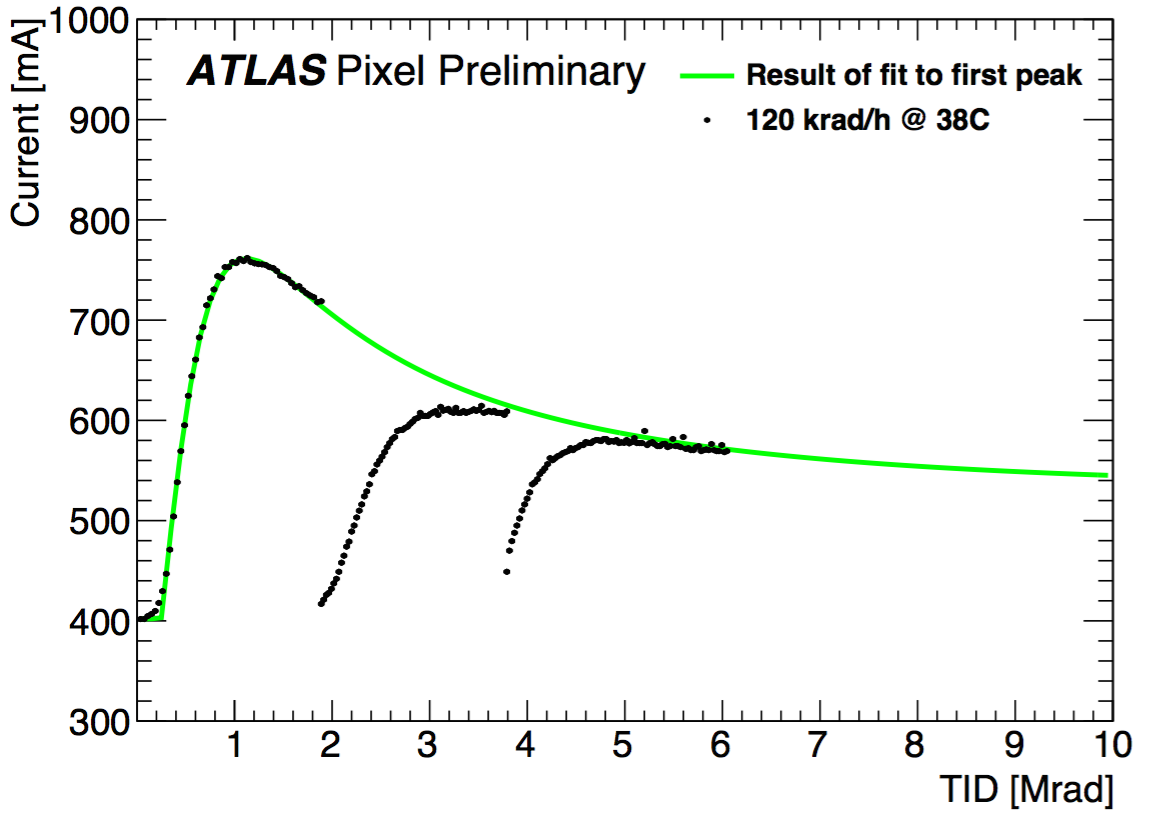
\includegraphics[height=7.5cm,keepaspectratio]{totaldose.png}
%  \caption[トータルドーズ効果と漏れ電流の関係]{トータルドーズ効果と漏れ電流の関係 \cite{totaldoze}。}
%  \label{fig:totaldoze}
%\end{figure}


これまで、電荷較正後の補完作業は1人の担当者による手作業で行われていた。Run3からは放射線損傷による影響がさらに大きくなることから、電荷較正の頻度が10日に1度程度になる予定であり、この作業を行うのは非常に労力が伴う。さらに、これまで行っていた補正では手作業による補正であることから、担当者によっては異なる値を補完してしまうことがある。本研究では適切な欠損の補完処理を行うよう、例外をアルゴリズムとして抽出・処理する自動解析ツールの開発を行った。次節からその詳細について説明する。


%------------------------------------------------------------------------------------------------------------------------
\section{電荷較正の補正}
\label{sec:calibhosei}
%------------------------------------------------------------------------------------------------------------------------
\fref{fig:calibhikaku}の右図に示すように、電荷生成のための回路の個体差により正しい電荷が生成できず、誤ったToTを持つ電荷を用いて電荷較正を行ってしまう場合がある。この様な点を取り除くために、これまでは\eref{eq:averagedistance}を用いて電荷較正結果の評価を行っていた。
\begin{equation}
  \label{eq:averagedistance}
  \Delta d = \sum_{i=1}^{N} \frac{ToT_{true, i} - ToT_{fit, i}}{N}
\end{equation}
ここで、$N$は電荷較正に使われた試験電荷の数であり、$ToT_{true, i}$および$ToT_{fit, i}$はそれぞれ電荷較正に使用された試験電荷のについての$i$番目のToT、電荷較正式によるフィッティングから得られる$i$番目のToTである。
%電荷較正結果の評価のために、全てのFEチップにおいて計算した$\Delta d$の分布を\fref{fig:averagedistance}に示す。
この評価では$\Delta d > 0.5$の場合、電荷較正に正しく生成されいない試験電荷が存在するとし、そのフィッティング結果を取り出して補正を行っており、2018年9月における電荷較正では、約250個の正しく電荷が生成されていないフィッティング結果が見つかり、その補正を行った。

%\begin{figure}[tbp]
 % \centering
 % 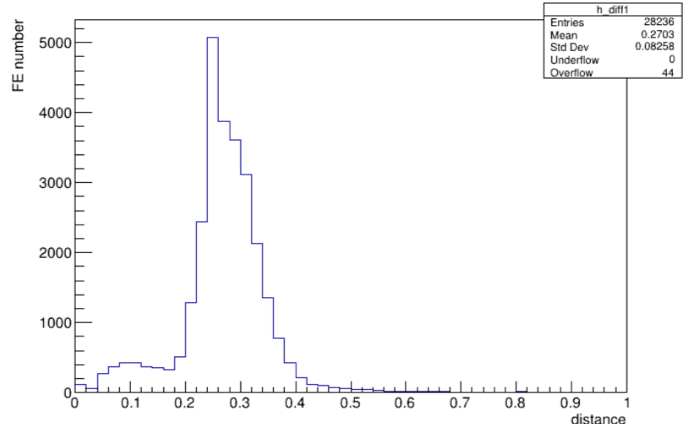
\includegraphics[height=6cm,keepaspectratio]{averagedistance.png}
 % \caption[電荷較正結果の評価のための$\Delta d$の分布]{電荷較正結果の評価のための$\Delta d$の分布。}
%  \label{fig:averagedistance}
%\end{figure}

\eref{eq:averagedistance}の評価方法は、電荷較正に使う試験電荷の数によって大きさが変化するものである。そのため、問題のある試験電荷を取り除いた後の電荷較正結果の評価のための基準値は、$0.5$とは別の値を用いる必要がある。自動補正を行う際、電荷再較正を行う度に基準値を変更するのは非常に困難である。
そこで、本研究で新たな評価基準を導入し、それを用いた電荷再較正の自動化アルゴリズムの開発を行った。


%------------------------------------------------------------------------------------------------------------------------
\subsection{電荷較正結果の評価方法}
%------------------------------------------------------------------------------------------------------------------------
電荷較正結果を評価するための新たな基準を以下に示す。
\begin{itemize}
  \item[]\textbf{試験電荷とフィット結果から得られる電荷の差が、試験電荷の5\%以上であれば問題のある試験電荷とみなす}
\end{itemize}
上記の評価基準は、ピクセル検出器における主な測定対象であるMIP粒子の検出感度から決定した。MIP粒子がピクセル検出器に落とす電荷量の分布を\fref{fig:mipdist}に示す。荷電粒子がシリコンセンサーに落とす電荷の分布はLandau分布に従う。MIP粒子がシリコンセンサーに落とす電荷量の測定分解能は$15\%$程度である。上記の基準を満たしていれば、電荷較正により得られる電荷量の揺らぎが\fref{fig:mipdist}におけるランダウ分布の揺らぎより十分小さく抑制することができる。

\begin{figure}[tbp]
  \centering
  \includegraphics[height=7cm,keepaspectratio]{mipdist.png}
  \caption[MIP粒子がピクセル検出器に落とす電荷量]{ピクセル検出器の$250\ \si{\micro m}$あたりのピクセル検出器にMIP粒子が落とす電荷量。現行ピクセル検出器におけるセンサーの厚みは$250\ \si{\micro m}$のため、MIP粒子が落とす電荷量に相当する。クラスターはnormalピクセルのみからつくられるものであり、ピクセルの短方向($50\times400\ \si{\micro m^2}$[行$\times$列]の$50\ \si{\micro m}$の方向)に2つピクセルから構成されるクラスターのみのデータである。}
  \label{fig:mipdist}
\end{figure}

%上記の基準を満たしていれば、MIP粒子がシリコンセンサーに落とす電荷の測定精度$5\%$であり、電荷較正による分解能が\fref{fig:mipdist}におけるランダウ分布の揺らぎより十分小さくできる。

また、この基準は各試験電荷について個別の評価を行っているため、試験電荷の数に依存せず電荷再較正の自動処理により適した評価方法である。\fref{fig:partialdistance}にB-Layerの全FEチップについて計算した試験電荷と電荷較正結果から得られる電荷の差の分布を示す。この分布において、試験電荷とから得られる電荷の差と試験電荷の比が$5\% $より大きいFEチップについて電荷較正結果の補正を行う。次項において、電荷再較正の処理方法について説明する。

\begin{figure}[tbp]
  \centering
  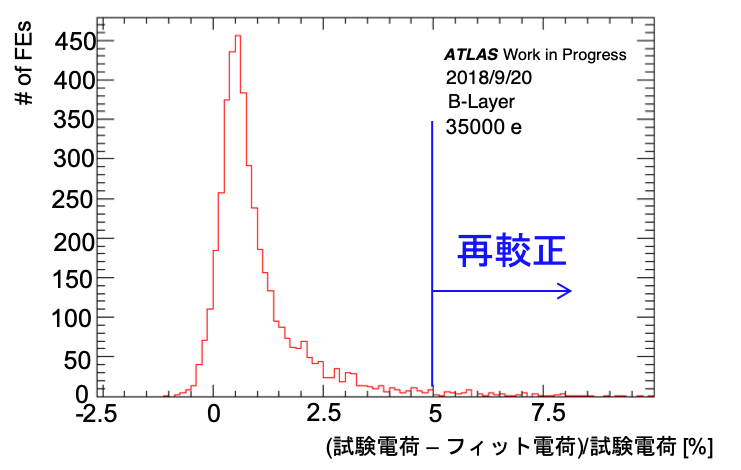
\includegraphics[height=7cm,keepaspectratio]{partialdistance.png}
  \caption[B-Layerの全FEチップについて計算した試験電荷と電荷較正結果から得られる電荷の差の分布]{B-Layerの全FEチップについて計算した試験電荷と電荷較正結果から得られる電荷の差の分布。}
  \label{fig:partialdistance}
\end{figure}


%------------------------------------------------------------------------------------------------------------------------
\subsection{電荷再較正の自動化アルゴリズム}
%------------------------------------------------------------------------------------------------------------------------
上記の評価基準を用いて電荷再較正を自動で行うツールを作成した。解析処理を行うために、CERNが提供している解析フレームワークであるROOTを使用している。電荷較正のために作成されたROOTの解析ツールを改良し、電荷較正後に結果の評価および再較正を行うプログラムを追加した。
作成したツールの処理の流れを\fref{fig:saikouseiflow}に示す。

\begin{figure}[tbp]
  \centering
  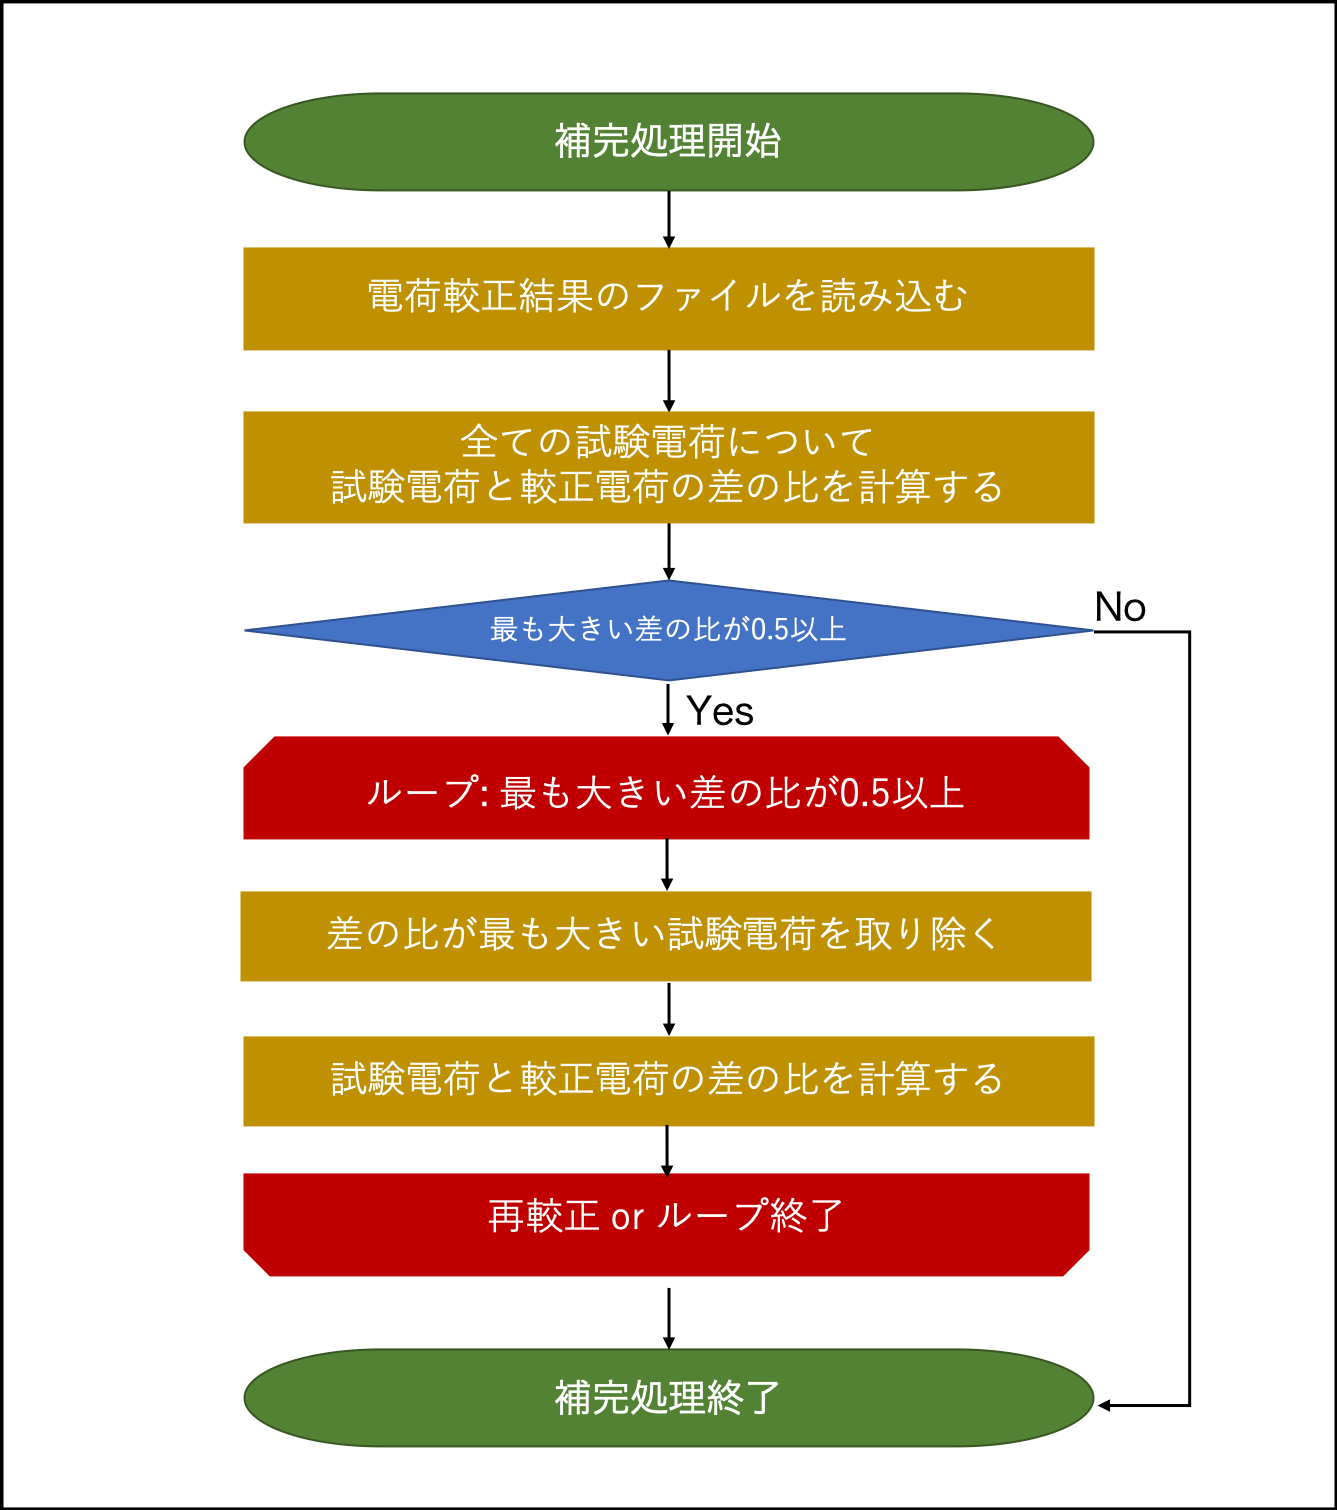
\includegraphics[height=10cm,keepaspectratio]{saikouseiflow.png}
  \caption[電荷較正結果を再較正するツールの処理の流れ]{電荷較正結果を再較正するツールの処理の流れ。}
  \label{fig:saikouseiflow}
\end{figure}


\fref{fig:saikouseiflow}に示したループの処理で電荷較正から得られる電荷と試験電荷の差が0.5\% 以内に収束するまで再較正の処理を行う。これにより問題のある試験電荷を全て取り除いて電荷較正を行うことができる。電荷再較正のアルゴリズムを用いて問題のある試験電荷を取り除き再構成した結果を\fref{fig:calibhosei}に示す。この右図より、問題があると考えられる$30000\ \si{e}$および$35000\ \si{e}$の試験電荷を取り除き、正しい電荷再較正結果が得られる。

\begin{figure}[tbp]
  \begin{minipage}[b]{0.5\linewidth}
    \centering
    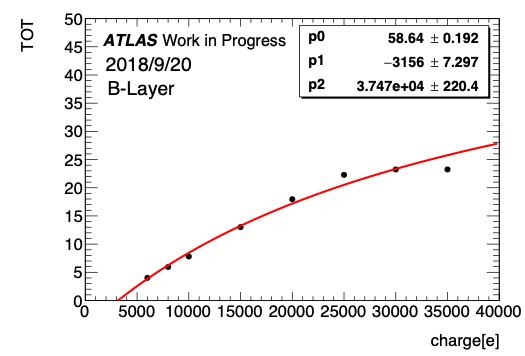
\includegraphics[keepaspectratio, scale=0.85]{calibhoseimae.png}
  \end{minipage}
  \begin{minipage}[b]{0.5\linewidth}
    \centering
    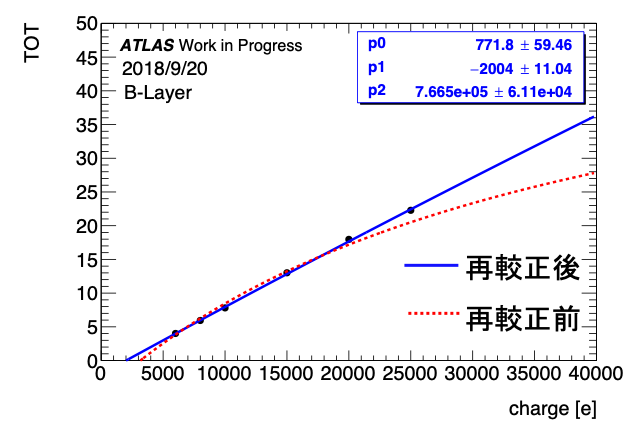
\includegraphics[keepaspectratio, scale=0.72]{calibhoseigo.png}
  \end{minipage}
  \caption[電荷再較正前後のフィッティング結果]{電荷再較正前(左図)と後(右図)のフィッティング結果。}
  \label{fig:calibhosei}
\end{figure}


%------------------------------------------------------------------------------------------------------------------------
\section{データに欠陥が含まれる場合の補完}
\label{sec:kessonhosei}
%------------------------------------------------------------------------------------------------------------------------
これまではピクセルモジュール内の一部のFEチップが欠陥しているデータがある場合には、最も近いFEチップから値をコピーすることにより補完していた。しかし、ピクセル検出器におけるモジュールは近いFEチップは2つまたは3つあるため、どの値を用いて補完を行うかは担当者の裁量によるものであった。より適切な方法を用いて自動処理を行うために、以下の二つの補完方法を導入する。
\begin{itemize}
  \item[1. ] 同一FEチップ上の他のピクセルタイプの平均値を用いた補完(\fref{fig:houhouhou}の左)
  \item[2. ] 欠陥している部分を除いた全てのFEチップの平均値を用いた補完(\fref{fig:houhouhou}の右)
\end{itemize}
各パラメータの補完のため、2つの補完方法の内、どちらがより実際の値を再現するかの評価を行った。

\begin{figure}[tbp]
  \begin{minipage}[b]{0.45\linewidth}
    \centering
    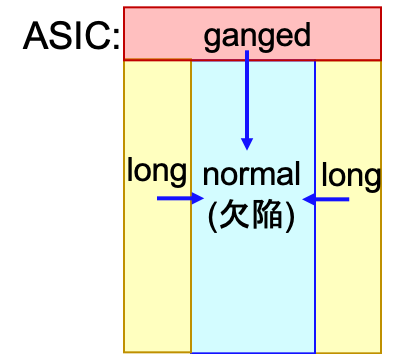
\includegraphics[keepaspectratio, scale=0.6]{houhousame.png}
  \end{minipage}
  \begin{minipage}[b]{0.55\linewidth}
    \centering
    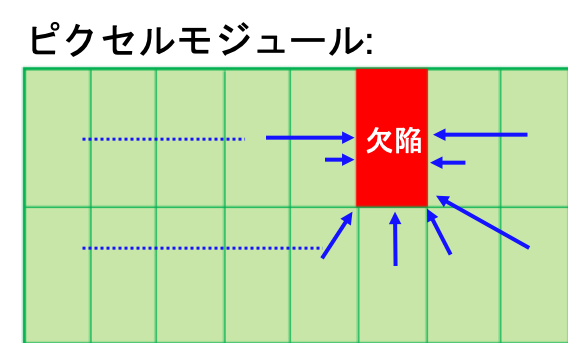
\includegraphics[keepaspectratio, scale=0.7]{houhoudiff.png}
  \end{minipage}
  \caption[データ欠陥の補完方法]{データ欠陥の補完方法についての概念図。左図はあるFEチップにおいて、normalピクセルの値が欠陥している場合に、longおよびgangedピクセルから補完することを示す。右図は欠陥の補完のために、異なるFEチップにある値を用いて補完することを示す。}
  \label{fig:houhouhou}
\end{figure}


%------------------------------------------------------------------------------------------------------------------------
\subsection{評価方法}
%------------------------------------------------------------------------------------------------------------------------
補完方法の評価のため、電荷較正結果に含まれるパラメータの1つが欠陥していると仮定し、そのパラメータと補完により得られる値の差を計算し分布の作成を行った。評価を行う際、2018年9月に行われた電荷較正の結果を用いた。IBLおよびピクセル検出器の全ての層について評価を行ったが、全ての層について同様の結果が得られたため、以下ではB-Layerの結果のみについての議論を行う。

%------------------------------------------------------------------------------------------------------------------------
\subsection{評価結果と考察}
%------------------------------------------------------------------------------------------------------------------------

前節において説明した方法を用いて、補完方法の評価を行った。\fref{fig:kekkanthreshold}はNormalピクセルにおけるThresholdについての評価結果を表す。この結果から、Threshold値は補完方法1の同一FEチップにおける別のピクセルタイプから得られる平均値を用いて補完した場合の方が、より精度良く補完を行うことがわかる。これはThresholdのチューニング方法によるものだと考えられる。チューニングではあるFEチップにおけるピクセル全体にglobalチューニングを行った後、各ピクセルごとにlocalチューニングを行う。初めにglobalチューニングを行うことから、別のFEチップの値を用いて補完するより、同一FEチップの値を用いて補完する方が実際の値に近い値を用いた補完を行うことができる。

\fref{fig:kekkannoise}はNormalピクセルにおけるThresholdのノイズについての評価結果を表す。この結果から、ノイズは補完方法2の別のFEチップにおける同一ピクセルタイプから得られる平均値を用いて補完した場合の方が、より精度良く補完を行うことができるとわかる。gangedピクセルはnormalピクセル2つをワイヤーで接続しているため、normalピクセルに比べてノイズが大きくなる。さらに、longピクセルは長方形の一片の長さがnormalピクセルの1.5倍あるため、normalピクセルと比べてピクセル間に生じるキャパシタンスが大きくなる。これによりFEチップ内の回路にノイズが加わり、longピクセルのノイズはnormalピクセルよりもノイズが大きくなる。


\begin{figure}[tbp]
  \begin{minipage}[b]{0.5\linewidth}
    \centering
    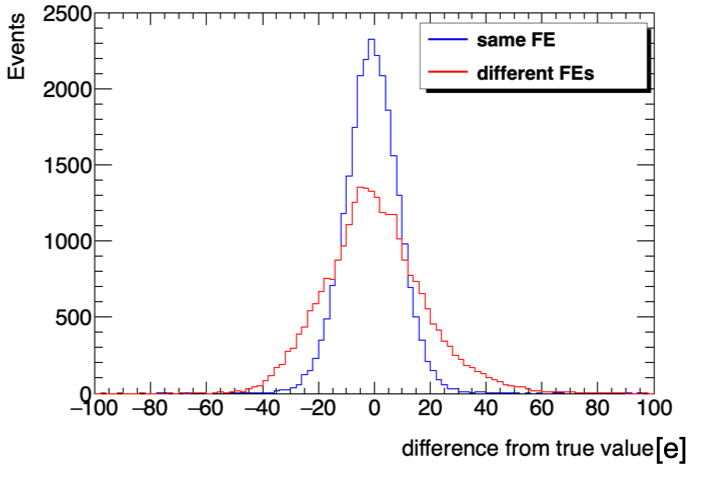
\includegraphics[keepaspectratio, scale=0.6]{kekkanthreshold.png}
    \caption[Thresholdの評価結果]{Thresholdの評価結果。同一FEチップにおける平均値の分布(青色)は、異なるFEチップの値の平均値の分布(赤色)よりのピークが鋭くなっている。}
    \label{fig:kekkanthreshold}
  \end{minipage}
  \begin{minipage}[b]{0.5\linewidth}
    \centering
    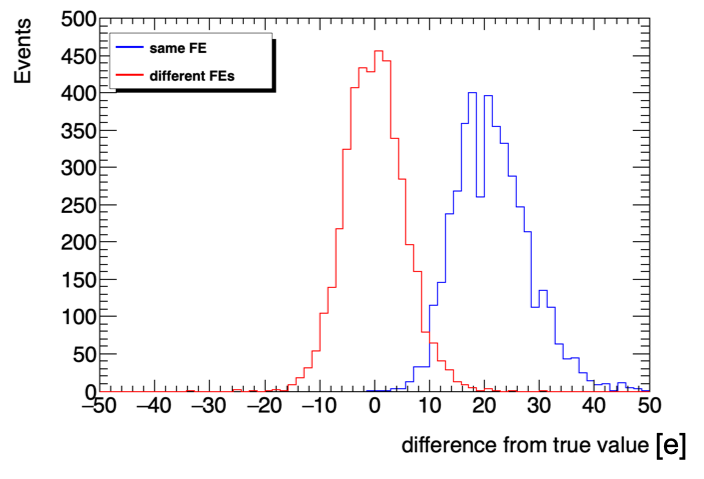
\includegraphics[keepaspectratio, scale=0.6]{kekkannoise.png}
    \caption[Thresholdのノイズの評価結果]{Thresholdのノイズの評価結果。同一FEチップの平均値の分布(青色)は、ピークの中心値がゼロからずれている。\\}
    \label{fig:kekkannoise}
  \end{minipage}
\end{figure}

他のパラメータについては\fref{fig:kekkannoise}と同様に、補完方法1と2の分布のピークの中心値が異なる結果が得られたため、補完方法2を用いることにより実際の値に近い値を再現できると考えられる。

%------------------------------------------------------------------------------------------------------------------------
\subsection{欠陥補完のための解析ツール}
%------------------------------------------------------------------------------------------------------------------------
上記の評価結果を用いて、自動で補完処理を行うツールの作成を行った。欠陥補完のための処理の流れを以下に示す。
\begin{itemize}
  \item[1. ] 補完結果のファイルを読み込む
  \item[2. ] 結果ファイル内の全てのモジュールについて、補完方法1および2を用いて値の補完を行う
  \item[3. ] スキャンが行われていないモジュールがあれば、一つ前の電荷較正結果の値をコピーし補完する
  \item[4. ] 補完結果をデータベースにアップロード可能なフォーマットに整形する
\end{itemize}

電荷較正結果をデータベースにアップロードするためには、電荷較正が行われていないモジュールの結果についても結果ファイル内に書き込む必要がある。そのため、処理の流れの3のように、電荷較正が行われていないモジュールについては1つ前の電荷較正結果から値をコピーすることにより補完を行う。また、データベースへアップロードするためには補完結果のファイルの中身を整形する必要があり、その処理についても補完処理を行うツールの最後に行う。

%------------------------------------------------------------------------------------------------------------------------
\section{自動補完のための解析ツール}
\label{sec:kaisekitool}
%------------------------------------------------------------------------------------------------------------------------
\ref{sec:calibhosei}節および\ref{sec:kessonhosei}節で示した補完方法を用いて自動で補完処理を行う解析ツールの開発を行った。解析ツールが行う処理の流れを以下に示す。

\begin{itemize}
  \item[1. ] \fref{fig:saikouseiflow}の流れで電荷較正および再較正
  \item[2. ] CERNのデータベースにアクセスし、1つ前の電荷較正結果の履歴を取得
  \item[3. ] \ref{sec:kessonhosei}節に示した解析ツールを用いて欠陥の補完および結果ファイルの整形
  \item[4. ] 補完についてのまとめファイルを出力
\end{itemize}

処理の流れの4番目に示すように、電荷再較正および欠陥の補完を行った後にどの様に補完を行ったかについてのまとめファイルを出力する。まとめファイルの例を\cref{code:matomefile}に示す。まとめファイルのはじめに、どのように補完が行われるかを記し、その後に補完結果が確認できる様にした。

\begin{lstlisting}[caption=解析ツールにより出力される補完結果のまとめ。,label=code:matomefile, language=C++]
##===========================================================================
## This file shows the way to recover data loss and calibration failure.
##
## How to recover parameters:
## 1. If there is a data loss in output data:
##   - Case1: Partial loss in a module
##     - Threshold: Recover using average of same FE
##     - Others:    Recover using average of different FEs
##   - Case2: All values loss in a module
##     - Previous scan result is used for the recovery
##
## 2. If there is a calibration failure:
##   - Remove incorrect injected charge & refitting
##   - Removed charges are listed in order of deletion
##
## Example of an output for a module:
##   L0_B08_S1_A6_M2A:
##   I2: [ normal threshold ], [ ] <--- Parameters that become '0' is listed
##   I8: [ ], [ 30000 40000 ] <-------- Injected charges that removed is listed
##
##===========================================================================

~~~~~~~~ Summary for the recovery ~~~~~~~~
1. Number of parameters that were 0
Number of FEs with all values zero: 11
normal threshold: 11
normal noise: 11
normal sigma: 11
normal intime: 27
fit_normal A: 11
fit_normal E: 11
fit_normal C: 11
quality/unused unused: 11
quality/unused fit_quality: 11

2. Number of FEs that had bad fits
B-Layer: 0
Layer1: 0
Layer2: 0
Disk: 5

3. Number of modules that were not scanned
B-Layer: 286
Layer1: 494
Layer2: 676
Disk: 6
~~~~~~~~~~~~~~~~~~~~~~~~~~~~~~~~~~~~~~~~~~

D1A_B01_S1_M1:
I0 [ normal threshold ], [ ]
D1A_B01_S1_M2:
D1A_B01_S1_M3:
I8: [ ], [ 30000, 40000 ]
\end{lstlisting}



%------------------------------------------------------------------------------------------------------------------------
\section{解析ツールの運用}
\label{sec:unnyou}
%------------------------------------------------------------------------------------------------------------------------

Run3におけるATLAS実験のためのモンテカルロシミュレーションのサンプル作成のために、2021年9月に電荷較正のためのデータ取得が行われた。電荷較正結果をデータベースにアップロードするために、本研究で作成した解析ツールを用いて電荷較正結果を作成した。以下では、電荷較正における補完結果をまとめる。


%------------------------------------------------------------------------------------------------------------------------
\subsection{補完のまとめ}
\label{sec:matome}
%------------------------------------------------------------------------------------------------------------------------
電荷較正結果と同時に出力されるファイルを用いて、補完内容の確認を行なった。\tref{tab:hokannmatome}に補完結果のまとめを示す。この結果から、各モジュールに存在した欠陥を取り除き、値の再現ができたと考えられる。表中に示すように、B-Layerにおける再較正を行ったFEチップの数は他の層と比較して非常に多くなった。これについて次節にて説明する。

\begin{table}[tbp]
  \begin{center}
    \caption[RUN3に向けた電荷較正補完のまとめ]{RUN3に向けた電荷較正補完のまとめ。次節に示すように、電荷較正および再較正はデータ取得に大きく影響を与えると考えられる電荷量の領域($>5000\ \si{e}$)のみを用いて行った。}
    \label{tab:hokannmatome}
    \begin{tabular}{|l||c|c|c|c|}
    \hline
      補完項目 & B-Layer & Layer1 & Layer2 & Disk  \\
    \bhline{1.5pt}
      スキャンされなかったモジュール数  & 14 & 18 & 40 & 6 \\
    \hline
      欠陥していたFEチップの数  & 18 & 46 & 38 & 11 \\
    \hline
      部分的に0となっていたパラメータ数  & 0 & 6 & 8 & 3 \\
    \hline
      再較正を行なったFEチップの数 & 179 & 1 & 9 & 5 \\
    \hline
    \end{tabular}
  \end{center}
\end{table}


%------------------------------------------------------------------------------------------------------------------------
\subsection{Run3に向けた電荷較正結果の再較正}
\label{sec:saisinsaikousei}
%------------------------------------------------------------------------------------------------------------------------

2021年9月に行われた電荷較正で用いた試験電荷の最小値は$3000\ \si{e}$であり、$10000\ \si{e}$までは$500\ \si{e}$ずつ電荷量を変更させてToTスキャンを行い、それ以降は$12000,\ 14000,\ 16000,\ 18000,\ 20000,\ 25000\ \si{e}$の試験電荷を用いてToTスキャンを行う。全ての試験電荷を用いて電荷較正およびその再較正を行った結果を\fref{fig:blayerba}に示す。右図は全ての点を用いて電荷較正を行った結果であり、右図はその再較正結果である。再較正では$5000\ \si{e}$以下の試験電荷を全て取り除くことにより再較正が完了する。

\begin{figure}[tbp]
  \begin{minipage}[b]{0.5\linewidth}
    \centering
    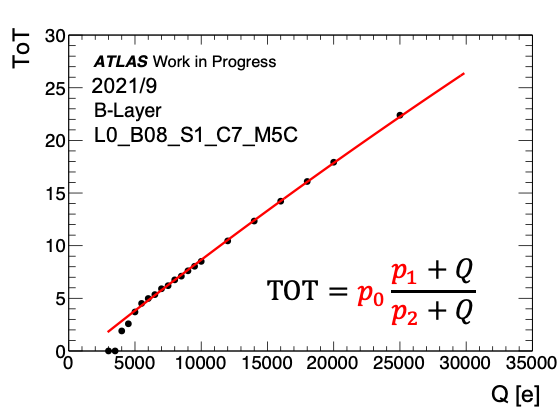
\includegraphics[keepaspectratio, scale=0.8]{blayerbefore.png}
  \end{minipage}
  \begin{minipage}[b]{0.5\linewidth}
    \centering
    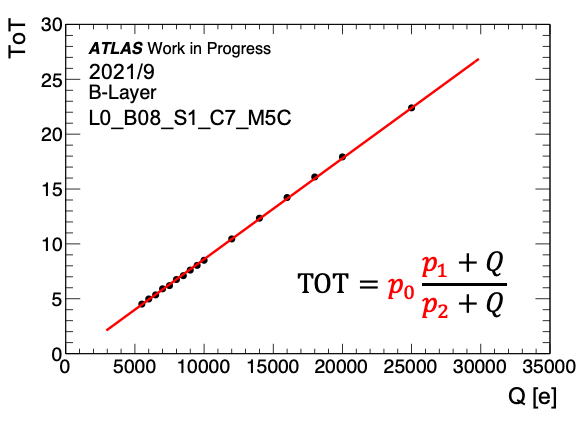
\includegraphics[keepaspectratio, scale=0.78]{blayerafter.png}
  \end{minipage}
  \caption[2021年9月に行われたB-Layerについての電荷較正結果]{2021年9月に行われたB-Layerについての電荷再較正結果。左図は再較正前のフィット結果であり、右図は基準を満たさない点を取り除き再較正を行った後の結果である。}
  \label{fig:blayerba}
\end{figure}

この電荷較正におけるThresholdの値は$3500\ \si{e}$であり、タイムウォークが$25\ \si{ns}$となる電荷量は$5000\ \si{e}$程度である。そのため、$5000\ \si{e}$以下の点はタイムウォークの影響が大きくなることから、本来予想されるToTよりも小さいToTを出力してしまうと考えられる。電荷較正\eref{eq:calibration}は二次的な効果も含めた較正式であるが、このような効果を完全に再現できずにフィット結果がデータ点からずれてしまうと考えられる。

Run2までの電荷較正ではThresholdに近い電荷量を持つ試験電荷について$2000\ \si{e}$ずつ電荷量を変化させていたが、Run3に向けた電荷較正では$500\ \si{e}$ずつ電荷量を変化させ、ToTスキャンを行った。その結果、Threshold付近のToTと電荷量の関係がよく見えるようになり、小さい電荷量を持つ点を除く電荷再較正を行うようになった。この電荷再較正は全てのFEチップにおいて行われるため、補正結果のまとめファイルでは全てのFEチップに正しくない電荷が含まれるという出力が得られた。しかし、全てのFEチップに正しくないという結果は、\fref{fig:calibhosei}のような大きい電荷量でToTが飽和するような問題等をまとめファイルから見つけることが困難になってしまう。そこで、特出して悪い試験電荷が含まれる電荷較正結果のみを抽出できるように$5000\ \si{e}$より大きいの試験電荷のみを用いて電荷較正を行った。その結果のまとめが\tref{tab:hokannmatome}である。
%そこで、データ取得に大きく影響を与えると考えられる電荷量の領域を制限し電荷較正を行った。

%ピクセル検出器におけるデータ取得では、アナログ回路におけるThresholdとは別にToTの閾値を定義することによりヒット情報の記録を行う。ToTの閾値を超える信号を中心にクラスタリングを行い、そのクラスターにおける電荷量の測定やヒットの位置情報を測定する。Run3における電荷較正でのThresholdの値、ToTの閾値およびMIP粒子に相当するToTの値を\tref{tab:run3tuning}に示す。B-LayerにおいてはToTの閾値が$3$であり、ToTが$4$以上のヒットを用いてクラスタリングが行われる。そのため、$4\ \mathrm{ToT}$に相当する電荷量である$5000\ \si{e}$以上の試験電荷を用いて電荷較正を行った。また、他の層についてもB-Layerと同様の範囲を用いて電荷構成を行った。この試験電荷の範囲を用いて電荷較正結果の再較正を行った数が\tref{tab:hokannmatome}に記されている。

\begin{table}[tbp]
  \begin{center}
    \caption[Run3における電荷較正での各LayerにおけるThresholdの値、ToTの閾値およびMIP粒子に相当するToTの目標値]{Run3における電荷較正での各LayerにおけるThresholdの値、ToTの閾値およびMIP粒子に相当するToTの目標値。}
    \label{tab:run3tuning}
    \begin{tabular}{|l||r|r|r|}
    \hline
      Layer名  & Threshold & ToTの閾値 & MIP粒子に相当するToT  \\
    \bhline{1.5pt}
      B-Layer & $3500\ \si{e}$ & $3\ \mathrm{ToT}$ & $18\ \mathrm{ToT}\ (20\ \si{ke})$ \\
    \hline
      Layer1 & $3500\ \si{e}$ & $5\ \mathrm{ToT}$ & $30\ \mathrm{ToT}\ (20\ \si{ke})$ \\
    \hline
      Layer2 & $3500\ \si{e}$ & $5\ \mathrm{ToT}$ & $30\ \mathrm{ToT}\ (20\ \si{ke})$ \\
    \hline
      Disk & $3500\ \si{e}$ & $5\ \mathrm{ToT}$ & $30\ \mathrm{ToT}\ (20\ \si{ke})$ \\
    \hline
    \end{tabular}
  \end{center}
\end{table}

\tref{tab:hokannmatome}に示した電荷再較正を行ったFEチップについて、再較正で取り除いた点は$5500\ \si{e}$のみであり、\fref{fig:calibhosei}のような大きい電荷量でToTが飽和するような問題は確認されなかった。Run3に向けた電荷較正では試験電荷の最大値が$25000\ \si{e}$であり最大電荷量がRun2までの電荷較正より$10000\ \si{e}$小さくなったことから、\fref{fig:calibhosei}の原因である$V_\mathrm{cal}$の飽和が発生しなかったと考えられる。また、B-Layerにおける再較正を行ったFEチップの数は他の層と比較して非常に多くなった。これはB-Layerが他の層よりもMIP粒子に相当するToTが小さいことが原因だと考えられる。\tref{tab:run3tuning}に示すように、B-LayerにおいてMIP粒子に相当するToTは$18$であるのに対して、他の層では$30$である。そのため、B-LayerにおけるFEチップ内のアナログ信号のパルスは他の層と比べて波高が低いものとなり、$5500\ \si{e}$付近においてもタイムウォークによる影響が無視できず、B-Layernおける再較正を行ったFEチップの数が他の層より多くなると考えられる。


%\fref{fig:blayernew}に2021年9月に行われたB-Layerについての電荷較正のフィッティング結果の例を示す。\fref{fig:blayernew}に示すように、電荷較正では2つの構造が確認できた。
%
%\begin{figure}[tbp]
%  \begin{minipage}[b]{0.5\linewidth}
%    \centering
%    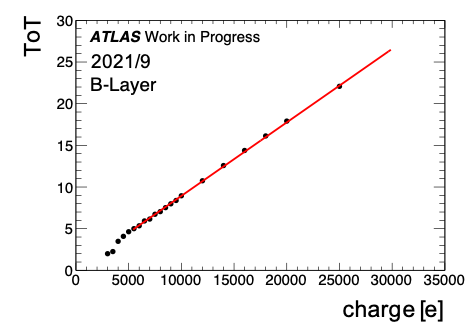
\includegraphics[keepaspectratio, scale=0.8]{blayernew1.png}
%  \end{minipage}
%  \begin{minipage}[b]{0.5\linewidth}
%    \centering
%    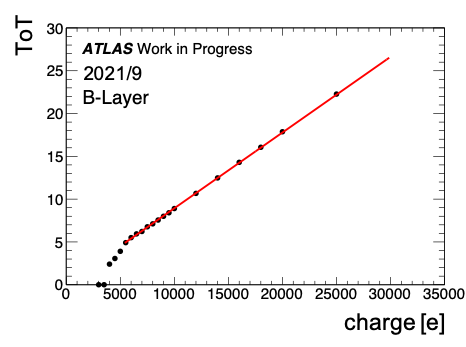
\includegraphics[keepaspectratio, scale=0.8]{blayernew2.png}
%  \end{minipage}
%  \caption[2021年9月に行われたB-Layerについての電荷較正結果]{2021年9月に行われたB-Layerについての電荷較正結果。}
%  \label{fig:blayernew}
%\end{figure}
%
%\fref{fig:blayernew}の左図は、Threshold値に近い小さい試験電荷量の点についてもToTから電荷量が再現できるものである。B-Layerではデジタル回路のThresholdとは別に、ToTの閾値が$3\ \si{ToT}$と定義されている。そのため、ToTが4以上であればデータの取得を行うが、そのようなものについても正しく較正できる。
%
%一方で、\fref{fig:blayernew}の右図は、Threshold値に近い小さい試験電荷量の点についてToTから電荷量の較正が正しくできないものである。ToTが5以上であれば、試験電荷から得られる点のフィット曲線上にあるため正しく較正できるが、$\mathrm{ToT}=4$の場合は、正しく較正できなくなってしまう。
%
%RUN2終了時までの電荷較正では電荷較正に用いられる試験電荷の最小値は$6000\ \si{e}$であり、電荷量を$2000\ \si{e}$ずつ変化させてデータの取得を行っていたため小さい試験電荷についての2つの構造が確認できていなかった。しかし、RUN3に向けた電荷較正では、放射線損傷による電荷収集の低下を保障するようThresholdを$3500\ \si{e}$まで引き下げられた。さらに、試験電荷の電荷量は$500\ \si{e}$ずつ変化させスキャンを行うため、このような違いが確認できるようになったと考えられる。そのため、小さい試験電荷を用いたToTスキャンについての理解を深め、\fref{fig:blayernew}の右図のような電荷較正結果が得られた際の電荷較正手法について再検討する必要があると考える。

%------------------------------------------------------------------------------------------------------------------------
\subsection{小さいToTに対する電荷較正}
\label{sec:minitot}
%------------------------------------------------------------------------------------------------------------------------

Run3に向けた電荷較正ではThreshold付近の電荷量を持つ試験電荷をより細かく生成した。電荷較正結果の再較正では$5000\ \si{e}$以下の試験電荷を全て取り除くことにより再較正が完了するため、$\mathrm{ToT}=5$以上の点は正しく電荷較正することが可能だが、それより小さいToTについては電荷較正のフィッティング結果と試験電荷の間に差異が現れた。この差異がデータ取得時の電荷較正にもたらす影響について本節で説明する。

ピクセル検出器におけるデータ取得では、タイムウォークの影響を抑えるためにIntime thresholdを用いており、1つのピクセルに対して電荷量がIntime threshold以下となる場合にはピクセルのヒット情報は記録されない。Run3に向けた電荷較正では、Intime threshldは約$4500\ \si{e}$となっているため、$\mathrm{ToT}\geq3$についてはヒット情報は記録されない。よって、小さいToTにおける電荷較正の差異がデータに影響を与えるのは$\mathrm{ToT}=4$のみである。

$\mathrm{ToT}=4$における電荷較正を評価するために、B-Layerの全FEチップについて電荷較正に用いたデータから$3.5 < \mathrm{ToT} < 4.5$となる点を取り出し、その電荷量と電荷較正\eref{eq:calibration}から得られる電荷量の比を計算した。その結果を\fref{fig:hikakukekkadayon}に示す。この図に示すように、データの電荷量と電荷較正\eref{eq:calibration}から得られる電荷量の比の分布には2つのピークが確認できた。これは、\fref{fig:blayernew}のように電荷較正結果のフィッティングには2つの構造があることだと考えられる。左の図の場合は、電荷較正結果が$\mathrm{ToT}=4$までデータ点を正しく再現できるものである。そのため、\fref{fig:hikakukekkadayon}において、データの電荷量と電荷較正\eref{eq:calibration}から得られる電荷量の比は$1$に近い値を持つ。一方で、\fref{fig:blayernew}の右図は、電荷較正結果が$\mathrm{ToT}=4$までデータ点を正しく再現できるものである。そのため、データの電荷量と電荷較正\eref{eq:calibration}から得られる電荷量の比は$1.2$に対応するものであり、この電荷較正結果がデータを再現するためにはフィッティング結果から得られる電荷量を$1.2$倍する必要がある。

\begin{figure}[tbp]
  \centering
  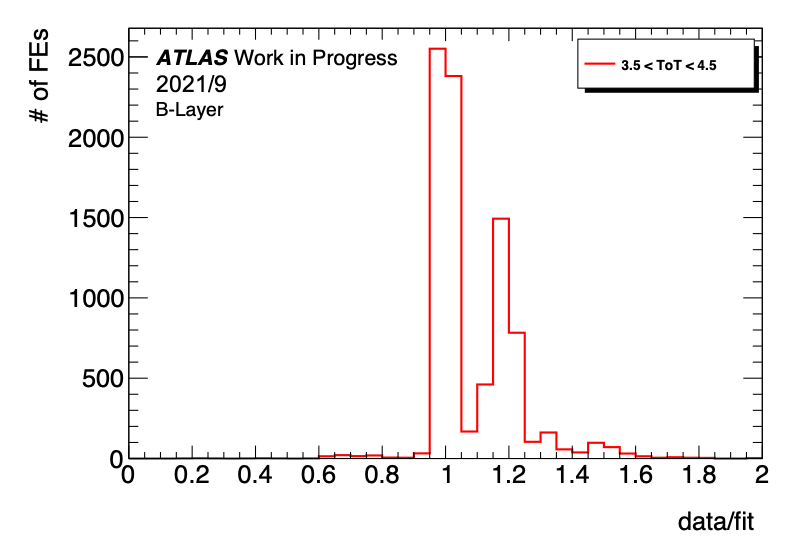
\includegraphics[height=7cm,keepaspectratio]{hikakukekkadayon.png}
  \caption[$\mathrm{ToT}=4$における電荷較正の評価結果]{$\mathrm{ToT}=4$における電荷較正の評価結果。横軸はデータの電荷量と電荷較正\eref{eq:calibration}から得られる電荷量の比を表し、縦軸はFEチップの数を表す。}
  \label{fig:hikakukekkadayon}
\end{figure}

\begin{figure}[tbp]
  \begin{minipage}[b]{0.5\linewidth}
    \centering
    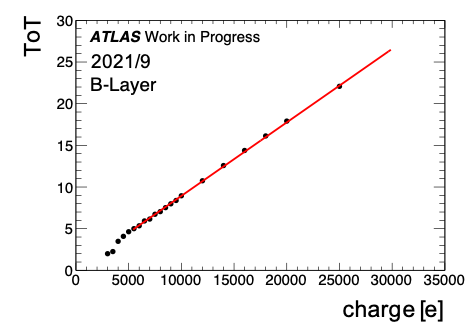
\includegraphics[keepaspectratio, scale=0.85]{blayernew1.png}
  \end{minipage}
  \begin{minipage}[b]{0.5\linewidth}
    \centering
    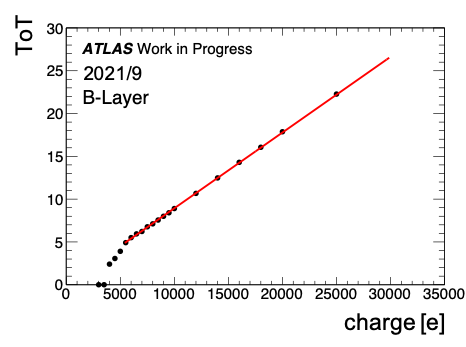
\includegraphics[keepaspectratio, scale=0.85]{blayernew2.png}
  \end{minipage}
  \caption[B-Layerの電荷較正結果における2つの異なる構造]{B-Layerの電荷較正結果における2つの異なる構造。左図は電荷較正結果が$\mathrm{ToT}=4$までデータ点を正しく再現できるものであり、右図は$\mathrm{ToT}=5$までデータ点を正しく再現できるものである。}
  \label{fig:blayernew}
\end{figure}

以上のことから、B-Layerについての電荷較正では、一部のFEチップについて$\mathrm{ToT}=4$の電荷較正結果を正確にデータ点を再現するためには、ToTから変換して得られる電荷量を約$1.2$倍する必要があることがわかった。しかし、以下の2つの理由から$\mathrm{ToT}=4$から得られる小さい電荷量の補正は行わないことに決定した。
\begin{itemize}
  \item MIP粒子に対する影響が大きくないと予想される\\
  荷電粒子が複数のピクセルにまたがりセンサーを通過すると、荷電粒子がセンサーに落とす電荷は複数のピクセルに分割される。そのため、荷電粒子の通過情報はヒットがあるピクセルのクラスターをつくることにより記録される。MIP粒子に相当する参照電荷量($20000\ \si{e}$)に対応するToTは$18$であるため、$\mathrm{ToT}=4$はクラスターの境界付近に現れる。$\mathrm{ToT}=4$に対する電荷量は約$20\%$ずれるため$1000\ \si{e}$程度の違いが現れるが、この電荷量はMIP粒子がシリコンセンサーに落とす電荷量のゆらぎ(\fref{fig:mipdist}参照)よりも十分小さい。そのため、$\mathrm{ToT}=4$から得られる小さい電荷の補正をしなくても、クラスターに対する影響は小さいと予想される。
  \item データベースを圧迫する\\
  全てのFEチップについて一律の倍率をかけることにより補正するのではなく、特定のFEチップにズレがあるため、そのFEチップのみに対して補正を行う必要がある。しかし、データベースにアップロードするパラメータの数は既に保存できる限界の量であり、これ以上増やすことができない。そのため、各FEチップに対して補正に必要な値を保存しておくことができず、小さい電荷を補正する値を保存しておくことができない。
\end{itemize}

\section{本章のまとめ}
本章では、電荷較正結果を確認し補完を行う解析ツールの概要を説明した。電荷較正の際に発生しうる問題は2種類ある。1つ目の問題は、電荷較正を行う際に正しい試験電荷が生成できないことである。この問題を検知するために電荷較正結果の新たな評価方法を導入し、問題のある試験電荷を順に取り除くアルゴリズムを開発した。2つ目の問題は、電荷較正結果に含まれるパラメータの欠陥である。これまでの補完方法は最も近いFEチップから値をコピーするという方法であり、担当者により異なる値による補完を行ってしまうことがある。そのため、本研究においてパラメータの最適な補完方法の評価を行った。その結果、Threshold値については同一FEチップにおける異なるピクセルタイプの平均、その他のパラメータについては異なるFEチップにおける同一ピクセルタイプの平均を用いることにより、より実際の値に近い値を再現できるという結果が得られた。この結果を利用し、電荷較正結果に含まれるパラメータの欠陥を自動補完する解析ツールの開発を行った。開発した解析ツールを用いて2021年9月に行われた電荷較正データを用いて、Run3モンテカルロシミュレーションサンプル作成のための電荷較正結果の作成を行った。

Run3に向けた電荷較正ではThreshold付近の電荷量を持つ試験電荷をより細かく生成した。そのため、Run2終了時では確認できなかった小さい電荷量について、データの電荷量と電荷較正式によるフィット結果から得られる電荷量に差異が確認された。その差異がデータ取得時にどの程度影響を与えるかの評価を行った。その結果、MIP粒子に対する影響が大きくないと予想されること、およびFEチップごとに補正のためのパラメータの値が異なり補正を行うようにするとデータベースを圧迫してしまうことから、$\mathrm{ToT}=4$から得られる小さい電荷量について補正を行わないことに決定した。




\newpage

%------------------------------------------------------------------------------------------------------------------------
\chapter{次世代ピクセルモジュールの量産}
\label{sec:singatapixel-devel}
%------------------------------------------------------------------------------------------------------------------------
RUN3に向けた現行ピクセルモジュールの測定準備に加え、ATLASではHL-LHCアップグレードに向けた内部飛跡検出器の総入れ替えのため、次世代ピクセルモジュールの開発が進められている。現在、ITkに搭載するピクセルモジュール量産の各組み立て工程における試験やそのシステム確立のため、試作器を用いたデモンストレーションが行われている。

日本では新型器量産の際に約$2000$個のモジュールを生産する予定である。次世代ピクセルモジュールの量産の際に、効率の良い量産と統合されたピクセルモジュール選定を行うため、品質試験結果を統合管理するシステムの開発が必要となる。


%------------------------------------------------------------------------------------------------------------------------
\section{次世代ピクセルモジュールの組み立て部品}
\label{sec:component}
%------------------------------------------------------------------------------------------------------------------------
量産工程は、各組み立て機関に届いたセンサーとASICから作られるベアモジュールとフレキシブル基板の接着から始まる。本節では各部品の詳細について説明する。


%------------------------------------------------------------------------------------------------------------------------
\subsection{ベアモジュール}
\label{sec:bare}
%------------------------------------------------------------------------------------------------------------------------

ベアモジュールはセンサーとASICをバンプ接合することにより作られる。クアッドモジュールではセンサー1枚に対してASIC1枚、トリプレットモジュールではセンサー1枚に対してASIC1枚から構成される。ベアモジュールは通過する粒子を検出する。センサーを通過した荷電粒子は電子・ホール対を生成し、それにより得られる信号をASICを用いて増幅・整形を行う。
%\fref{fig:bare}にベアモジュールの全体図を示す。
%\begin{figure}[tbp]
%  \centering
%  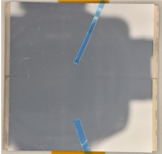
\includegraphics[height=5cm,keepaspectratio]{bare.png}
%  \caption[ベアモジュール]{ベアモジュールの全体図。センサー側から見たものであり、左右にASICがはみ出している。これはフレキシブル基板につながるワイヤーのためのパッド部分である。}
%  \label{fig:bare}
%\end{figure}

%現在行われている試作器の組み立てではRD53AというASICを用いている。


%------------------------------------------------------------------------------------------------------------------------
\subsection{フレキシブル基板}
\label{sec:flex}
%------------------------------------------------------------------------------------------------------------------------

フレキシブル基板はセンサーの裏側に接着、およびワイヤー配線によりASICと電気的に接続される。フレキシブル基板の全体図を\fref{fig:flex}に示す。フレキシブル基板は、以下の3つの役割を持つ。

\begin{figure}[tbp]
  \centering
  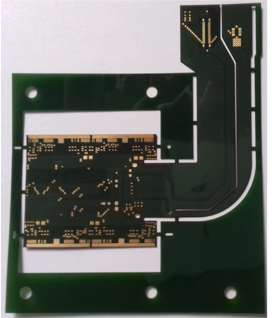
\includegraphics[height=6cm,keepaspectratio]{flex.png}
  \caption[フレキシブル基板]{フレキシブル基板の全体図\ \cite{itk}。}
  \label{fig:flex}
\end{figure}

\begin{itemize}
  \item ASICからの信号輸送  \\
  センサーから得られた信号はASICで増幅・整形され、フレキシブル基板に送られてくる。フレキシブル基板は送られてきた信号を後段のPCへ送る。
  \item 電源の供給 \\
  外部からの電源を、センサーとASICに供給する。センサーには、空乏領域を増加させるために$100\ \si{V}$程度のHV(\textbf{H}igh \textbf{V}oltage)をかける。ASICには、電源供給のために$5.6\ \si{V}$程度のLV(\textbf{L}ow \textbf{V}oltage)
  \item モジュールの制御システム(DCS: \textbf{D}etector \textbf{C}ontrol \textbf{S}ystem) \\
  モジュールの温度測定のために2つのNTC(\textbf{N}egative \textbf{T}emperature \textbf{C}oefficient)が配置されている。
\end{itemize}

%------------------------------------------------------------------------------------------------------------------------
\subsection{モジュールキャリア}
\label{sec:carrier}
%------------------------------------------------------------------------------------------------------------------------

モジュールキャリアはモジュールの運搬の際や品質試験を行う際に、モジュールを保護用の容器である。組み立てられたモジュールはASICとフレックス基板を繋ぐワイヤー部やセンサーの部分等が剥き出しになっているため、そのままの状態で品質試験を行うのはモジュール破損のリスクを伴う。モジュールキャリアでモジュールを保護することにより、安全に品質試験を行うことができる。

また、モジュールキャリアの別の役割として、モジュール周囲の湿度環境を一定に保つことが挙げられる。運転時に想定される最低温度は$-45\ \si{\degreeCelsius}$のため、品質管理試験ではペルチェ素子を用いた温度制御装置\footnote{KEKにおける次世代ピクセルモジュールの量産では、東工大を中心に開発している温度制御システムを用いる。}を用いて最低$-45\ [\si{\degreeCelsius}]$までモジュールの周囲温度を下げる。その際、ピクセルモジュールに結露が発生すると損傷のリスクを伴う。そのため、キャリア内に乾燥窒素ガスを流し込むことで氷点下におけるピクセルモジュールへの結露を防いでいる。

%------------------------------------------------------------------------------------------------------------------------
\section{次世代ピクセルモジュールの組み立て工程}
\label{sec:assemble}
%------------------------------------------------------------------------------------------------------------------------
\begin{figure}[tbp]
  \centering
  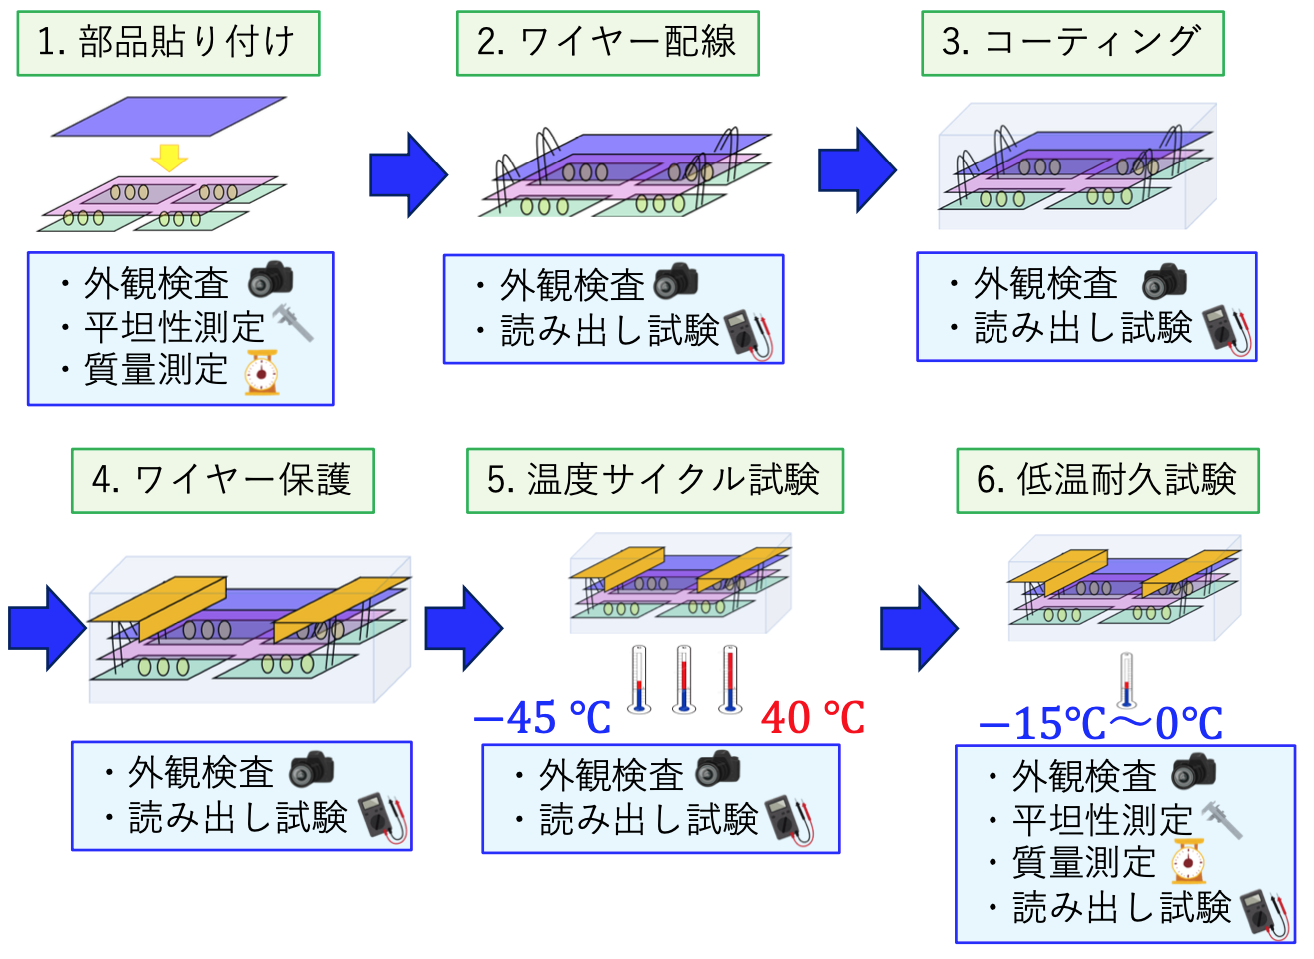
\includegraphics[height=2.3cm,keepaspectratio]{module_flow.png}
  \caption[ピクセルモジュールの組み立て工程]{ピクセルモジュールの組み立て工程。 }
  \label{fig:assemble}
\end{figure}


次世代ピクセルモジュールの組み立て工程を\fref{fig:assemble}に示す。組み立て工程ではフレキシブル基板とベアモジュールの接着から始まり、ワイヤー配線、パリレン高分子によるコーティング、ワイヤー保護を行いピクセルモジュールが完成する。その後、温度サイクル試験および低温耐久試験において、運転時に想定される温度環境において組み立てたモジュールが運用できるかの試験を行う。本節では、組み立て工程、およびモジュールの温度耐久についての試験についての説明を示す。

\subsubsection*{ベアモジュール・フレキシブル基板の接合}

モジュールの組み立て工程は、組み立て機関に輸送されたベアモジュールとフレキシブル基板の接合から始まる。輸送された各部品の受け取り時の品質試験を行った後、ベアモジュールとフレキシブル基板の接合を行う。専用治具を用いて行うことにより、フレックス基板の位置の交差は$\pm 50\ \si{\micro m}$、平面度は$25\ \si{\micro m}$の精度で接合を行うことができる。

\subsubsection*{ワイヤー配線}

フレキシブル基板とASICを電気的に接合し、電源の供給や、ASICからの信号を読み出すため、フレキシブル基板とASIC間をワイヤーで接続する。この組み立て工程をワイヤー配線と呼ぶ。ワイヤーは直径$25\ \si{\micro m}$でのアルミ製であり、1モジュールに対して約$500$本用いられる。ワイヤー配線後からは、モジュールの電気的な読み出しが行うことができるため、これ以降の全ての組み立て工程では読み出し試験を行い正常に動作するかの確認を行う。

\subsubsection*{パリレンコーティング}

モジュールのセンサーとASICの端の部分での放電を防ぐこと、湿気や化学物質からの保護を目的としてパリレンコーティングを行う。パリレンはパラキシリレン系ポリマーの略である。パリレンは結晶性が高く絶縁耐力に優れ、周波数に依存せず低い誘電率・誘電正接特性を持っており、湿気や腐食性ガスへの耐性も併せ持つ。


\subsubsection*{ワイヤー保護}

ワイヤーは直径$25\ \si{\micro m}$と非常に細いため、力が加わると損傷してしまう可能性がある。ITkを実装する際、モジュールとワイヤーの距離は$2\ \si{mm}$程度のため、モジュールのケーブルがワイヤーに触れてしまい読み出しが正常にできなくなる恐れがある。このような問題を避けるため、%\fref{fig:protection}に示すような
構造体を用いて、ワイヤーを保護する。

%\begin{figure}[tbp]
%  \centering
%  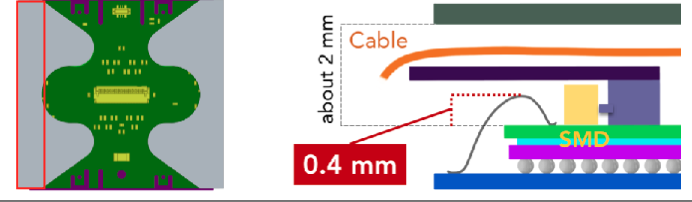
\includegraphics[height=4cm,keepaspectratio]{protection.png}
%  \caption[ワイヤー保護用の構造体]{ワイヤー保護用の構造体。炭素系の素材であるCFRPを用いて作成する。図を作る。 }
%  \label{fig:protection}
%\end{figure}

\subsubsection*{温度サイクル}

組み立てたモジュールに対して、ITk実装後にされる特異的な温度変化のサイクルを行い、その後もモジュールが正常な応答をするか試験をする。温度変化の際、モジュールの部品間の熱膨張の違いにより熱応力が生じ、それが原因でバンプ接合部に剥がれが生じてしまうことがある。このようの温度サイクルによるモジュールの損傷がないことを確認する必要がある。

ITkの運転の切り替えが年間$10$回以上あるため\CID{634}$10$年間の運転を想定すると$100$回以上の熱サイクルにさらされる。
そのため、量産における品質試験では、動作温度範囲$-45\ \si{\degreeCelsius}<T<40\ \si{\degreeCelsius}$の温度サイクルを$10$回、$-55\ \si{\degreeCelsius}<T<60\ \si{\degreeCelsius}$の温度サイクルを$1$回を行う。これらの温度サイクルの後にモジュールが正常に動作するかを確認するため、ASIC回路読み出し試験等を行う。モジュールの周囲温度を変える際には、恒温槽を用いて行う予定である。

\subsubsection*{低温耐久試験}

常温において
ITk運転におけるピクセルモジュールの周囲温度は$-15\ \si{\degreeCelsius}<T<0\ \si{\degreeCelsius}$である。組み立てたモジュールが低温環境下において長時間正常に動作することを確認する試験が低温耐久試験である。
低温耐久試験では、温度制御筐体を用いてモジュールの周囲温度を$-15\ \si{\degreeCelsius}$に保ちつつASICの回路読み出し試験を行う。読み出し試験は1時間に1度行われる。
\begin{figure}[tbp]
  \centering
  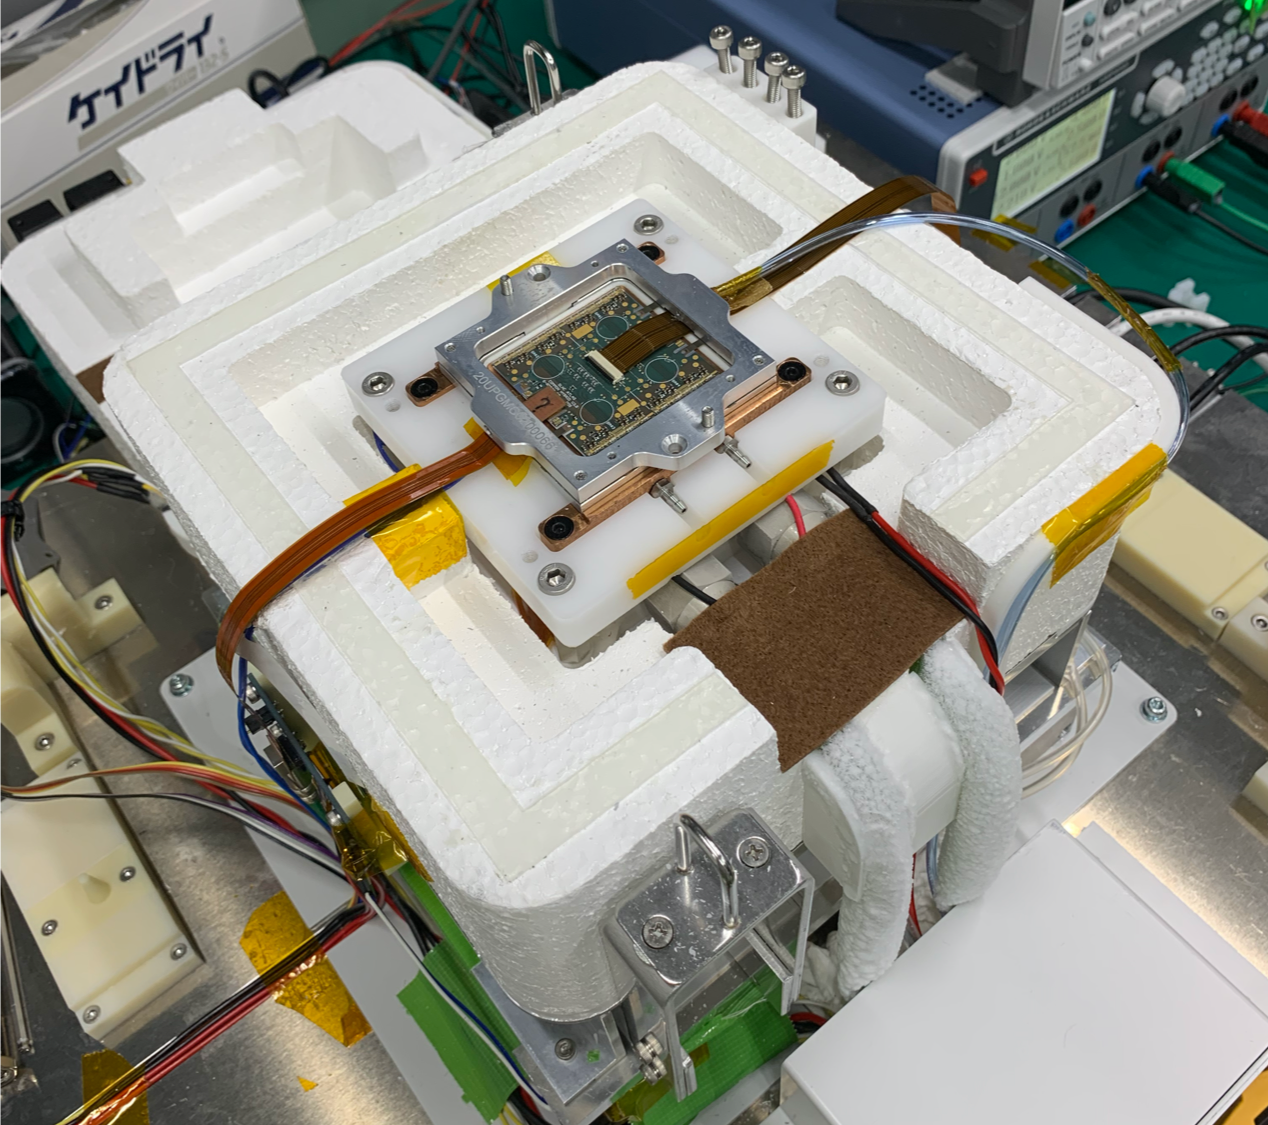
\includegraphics[height=7cm,keepaspectratio]{yomidashi.png}
  \caption[読み出し試験のセットアップ]{読み出し試験のセットアップ。この図は、温度制御筐体の蓋を開けた状態であり、測定時には蓋を閉めてモジュールの周囲を密閉し測定を行う。銀色のフレームがモジュールキャリアであり、その中にモジュールが設置されている。}
  \label{fig:yomidashi}
\end{figure}
%\begin{figure}[tbp]
%  \centering
%  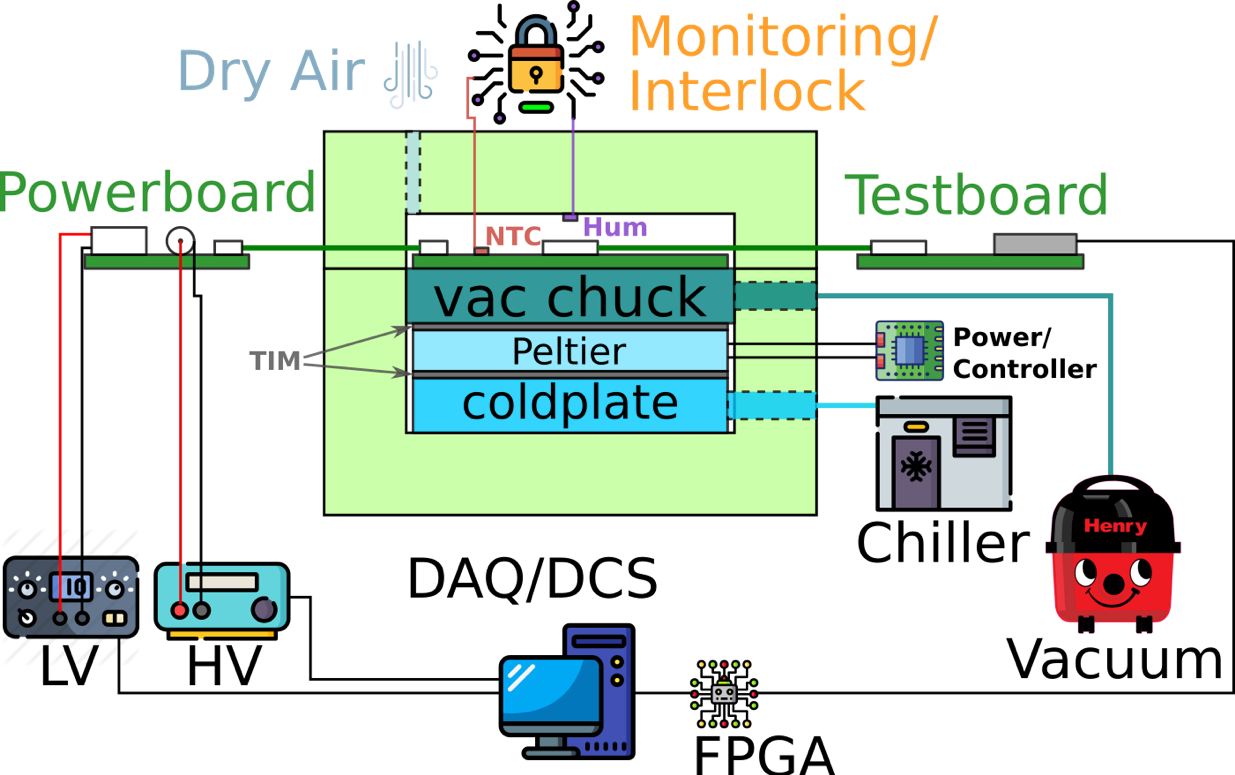
\includegraphics[height=7cm,keepaspectratio]{electrical_system.png}
%  \caption[読み出し試験の全体図]{読み出し試験の全体図。 }
%  \label{fig:electrical-system}
%\end{figure}

長時間放置しつつ読み出し試験を行うため、インターロックシステム、機器の遠隔制御、温度制御筐体の遠隔監視等の技術が必要となる。
%To do: ITk稼働の際にモジュール周囲温度が低い理由を二章に書く。\\
%\url{https://arxiv.org/pdf/2003.00055.pdf}, \\
%\url{https://iopscience.iop.org/article/10.1088/1748-0221/8/10/P10003/pdf}

%------------------------------------------------------------------------------------------------------------------------
\section{品質試験}
\label{sec:QCtest}
%------------------------------------------------------------------------------------------------------------------------

モジュールの各組み立て工程の後に、モジュールが正常に動作するかを確認するために品質試験を行う。\fref{fig:assemble}に示したように、モジュールの外観検査は全ての工程で行われ、ASICの回路読み出し試験はワイヤー配線後の全ての工程で行われる。本節では、各品質試験項目の詳細を以下に示す。



%------------------------------------------------------------------------------------------------------------------------
\subsection{外観検査}
\label{sec:visualinsp}
%------------------------------------------------------------------------------------------------------------------------
モジュールの表面(フレックス基板側)をカメラを用いて撮影し、モジュールに損傷や汚れ等がないことを目視で確認する。特に、ASICとフレックス基板を電気的に接合するためのワイヤーの接着位置が正しいか、断線がないかを確認することが重要である。目視で確認する際は、モジュール全体の高解像度画像を36(縦横$6\times6$)分割して得られる拡大画像を用いて細かく検査を行う。また、ワイヤー部分については約$500$本のワイヤーを目視で漏れなく検査することは困難且つ労力を伴うため、ワイヤーの断線や接続部分のずれを自動で検知するアルゴリズムの開発が進んでいる。



%------------------------------------------------------------------------------------------------------------------------
\subsection{平坦性測定}
\label{sec:metrology}
%------------------------------------------------------------------------------------------------------------------------
モジュール上の3次元位置座標を取得することにより、歪み具合や接着剤の厚み等を計算することができる。これにより、接着時のずれや接着剤の厚みに問題やモジュール輸送時にモジュールへの損傷等を確認することができる。
%\fref{fig:metrology}に平坦性測定結果を示す。

%\begin{figure}[tbp]
%  \centering
%  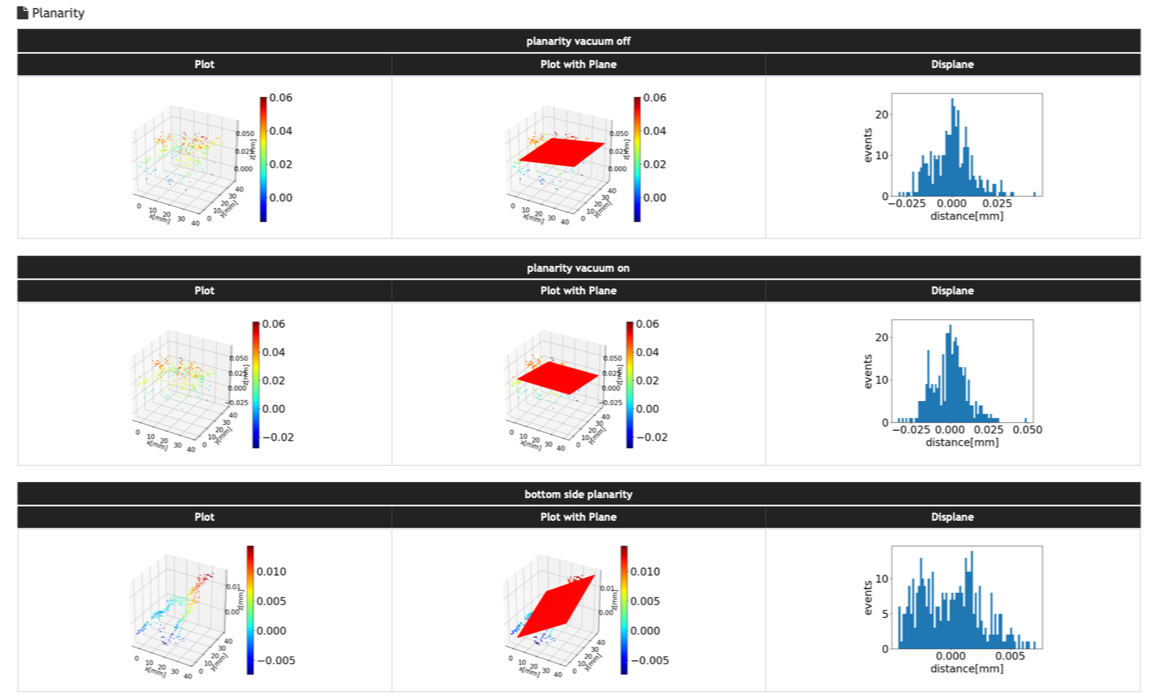
\includegraphics[height=7cm,keepaspectratio]{metrology.png}
%  \caption[平坦性測定の結果]{平坦性測定の結果 }
%  \label{fig:metrology}
%\end{figure}


%------------------------------------------------------------------------------------------------------------------------
\subsection{質量測定}
\label{sec:mass}
%------------------------------------------------------------------------------------------------------------------------
質量測定では、モジュール全体の質量を測定する。各工程における質量の差を計算することにより、接着剤の質量やワイヤーの合計質量等を取得することができる。

%------------------------------------------------------------------------------------------------------------------------
\subsection{ワイヤー強度検査}
\label{sec:mass}
%------------------------------------------------------------------------------------------------------------------------

ワイヤー配線により接続したワイヤーの強度を調べるため、専用の機械を用いてワイヤー部分に負荷を与える。


%------------------------------------------------------------------------------------------------------------------------
\subsection{センサー IV特性}
\label{sec:sensoriv}
%------------------------------------------------------------------------------------------------------------------------
センサーの電流-電圧特性を調べることにより、モジュール製造工程におけるセンサーの損傷やHVのショートを確認することができる。
プラナーセンサーでは、漏れ電流が$80\ \si{V}$で$2\ \si{\micro A}$、降伏電圧が$120\ \si{V}$、3Dセンサーについては漏れ電流が$25\ \si{V}$で$2\ \si{\micro A}$、降伏電圧が$35\ \si{V}$程度となるのが想定されうる結果である。また、測定はASICからの消費電力による発熱を避けるため、ASICへのLVを切った状態で行われる。
%Todo: 2章を書きつつ、センサーの詳細を調べ直す。


%------------------------------------------------------------------------------------------------------------------------
\subsection{SLDO VI特性}
\label{sec:sldovi}
%------------------------------------------------------------------------------------------------------------------------
ITk実装時には、モジュールを直列に並べて電源の供給を行う。そのため、各モジュールに対する電源は定電圧ではなく、供給電圧はつなげるモジュールの数に依存してしまう。
ASIC回路内部で一定の電圧を供給するために、SLDO(\textbf{S}hunt \textbf{L}ow \textbf{D}rop \textbf{O}ut)という制御回路を用いる。SLDO制御回路が供給電流の一部を用いてデジタル回路、アナログ回路の動作電圧を生成し、余剰電流はグランドに捨てられる。ASICには二つのSLDO制御回路が搭載されている。1つはデジタル回路用、もう1つはアナログ回路用に用いる。\fref{fig:sldoref}にASICへの電流と、入力電圧$V_\mathrm{in}$、アナログ回路の出力電圧$V_\mathrm{analog}$およびデジタル回路の出力電圧$V_\mathrm{digital}$の例を示す。
\begin{figure}[tbp]
  \centering
  \includegraphics[height=7cm,keepaspectratio]{sldoref.jpg}
  \caption[ASICへの電流と、入力電圧$V_\mathrm{in}$、アナログ回路の出力電圧$V_\mathrm{analog}$およびデジタル回路の出力電圧$V_\mathrm{digital}$の関係]{ASICへの電流と、入力電圧$V_\mathrm{in}$、アナログ回路の出力電圧$V_\mathrm{analog}$およびデジタル回路の出力電圧$V_\mathrm{digital}$の関係\cite{sldo}。}
  \label{fig:sldoref}
\end{figure}
この結果から、SLDO回路によりアナログ回路およびデジタル回路からの出力電圧は一定であり、制御回路が正常に動作していることがわかる。

さらに、SLDO VI特性についての品質試験を行う際には、ASICが低温においても正常に動作するかの試験も行う。モジュールの周囲温度を$-35\ \si{\degreeCelsius}$にし、デジタル回路の読み出し試験を行いモジュールが低温環境で動作することを確認する。正常に動作しない場合は$15\ \si{\degreeCelsius}$ずつ温度を上げて再び試験を行い、正常に動作を始める温度を記録する。温度を記録する際には、\tref{tab:gradesldo}に示すように各温度に対する階級を表す数値を用いて値の入力を行う。
\begin{table}[tbp]
  \begin{center}
    \caption[モジュール起動温度に対する階級値]{モジュール起動温度に対する階級値。}
    \label{tab:gradesldo}
    \begin{tabular}{|c|c|}
    \hline
      温度[$\si{\degreeCelsius}$] & 階級値 \\
    \bhline{1.5pt}
     $-35$ & $1$ \\
    \hline
     $-35 < T \leq -20$ & $2$ \\
    \hline
     $-20 < T \leq -5$ & $3$ \\
    \hline
     $-5 < T \leq 10$ & $4$ \\
    \hline
     $10 < T$ & $5$ \\
    \hline
    \end{tabular}
  \end{center}
\end{table}


%------------------------------------------------------------------------------------------------------------------------
\subsection{読み出し試験}
\label{sec:electricaltest}
%------------------------------------------------------------------------------------------------------------------------
モジュールに通電し、正常に読み出しができるか確認する。読み出し試験はITk運転時の温度環境を想定し、モジュールの周囲温度を変えつつ試験を行う。そのため、読み出し試験の際には低温耐久試験と同様に\fref{fig:yomidashi}の温度制御筐体を用いて試験を行う。設定温度は、低温におけるモジュール起動試験では$-35\ \si{\degreeCelsius}$ (正常に起動できない場合は$15\ \si{\degreeCelsius}$ずつ温度を上げて試験)、Threshold測定やToT測定等の通常の読み出し試験では$-20\ \si{\degreeCelsius}, 20\ \si{\degreeCelsius}$である。

読み出し試験に用いるDAQ(\textbf{D}ata \textbf{A}c\textbf{q}uisition)として、YARR(\textbf{Y}et \textbf{A}nother \textbf{R}apid \textbf{R}eadout)を用いる。YARRとはASIC読み出しように開発されている。YARRを用いて行う、モジュールの読み出し試験の項目を以下に示す。

\begin{itemize}
  \item Digitalスキャン \\
  各ピクセルについてのデジタル回路の応答を確認する。デジタル回路に試験用パルスを入射し、信号の応答数を測定する。
  \item Analogスキャン \\
  各ピクセルについてのアナログ回路の応答を確認する。アナログ回路に試験電荷を入射し、信号の応答数を測定する。
  \item Tresholdスキャン \\
  各ピクセルのThresholdを確認する。試験電荷を用いてSカーブのフィッティングを行い、Threshold値やノイズを測定する。
  \item ToTスキャン \\
  一定の試験電荷を各ピクセルに100回入射させ、その試験電荷に対するToTの値の測定を行う。
  \item Noiseスキャン \\
  各ピクセルのノイズを確認する。試験電荷を用いず、クロックによるトリガーで測定を行い、応答率を求める。
  \item Sourceスキャン \\
  放射線を照射し、各ピクセルの応答を確認する。これにより、シリコンセンサーとASIC間の接続の不具合等も確認することができる。
\end{itemize}

また、これらのスキャン項目に加え、ピクセルのチューニングも行うことがある。
\begin{itemize}
  \item Global threshold tuning \\
  ASIC全体のピクセルにおけるThresholdを一括チューニングする。
  \item Pixel threshold tuning \\
  各ピクセル毎にThreshold値チューニングする。
  \item Global ToT tuning \\
  ASIC全体のピクセルにおけるToT値を一括チューニングする。
  \item Pixel ToT tuning \\
  各ピクセル毎にToT値をチューニングする。
\end{itemize}


%\begin{table}[tbp]
%  \begin{center}
%    \caption[Powering overview for the on-detector system]{Powering overview for the on-detector system \cite{itk}}
%    \label{tab:powering}
%    \begin{tabular}{|l|l||l|}
%    \hline
%      \multirow{5}{*}{on-module} & モジュールへの電流値 & $5.6\ \si{A}$ \\
%    \cline{2-3}
%      & モジュールへのLV値 & $1.4\ \si{V}$ \\
%    \cline{2-3}
%      & モジュールの消費電力 & $7.85\ \si{W}$ \\
%    \cline{2-3}
%     & センサー & $< 0.1\ \si{W/cm^2}$ \\
%    \hline
%     \multicolumn{2}{|l||}{DCS power} & $0.15$-$0.28\ \si{W}$ per quad module \\
%    \hline
%     \multicolumn{2}{|l||}{Cooling system capability} & $0.7\ \si{W/cm^2}$ \\
%    \hline
%    \end{tabular}
%  \end{center}
%\end{table}


\begin{table}[tbp]
  \begin{center}
    \caption[ピクセル解析の評価基準一覧]{ピクセル解析の評価基準一覧 \cite{lingxin}}
    \label{tab:pixel-failure}
    \begin{tabular}{|l|l||l|}
    \hline
      評価名 & 読み出し試験項目 & 評価基準 \\
    \bhline{1.5pt}
      Digital Dead & Digital Scan & $\mathrm{Occupancy}<1\si{\%}$ of injections \\
    \hline
      Digital Bad & Digital Scan & $\mathrm{Occupancy}<98\si{\%}$ or $\mathrm{Occupancy}>102\si{\%}$ of injections \\
    \hline
      \multirow{2}{*}{Merged Bump} & Analog Scan & $\mathrm{Occupancy}<1\si{\%}$ of injections \\
       & Crosstalk Scan & $\mathrm{Occupancy}<80\si{\%}$ of $25\ \si{ke}$ injections \\
    \hline
      Analog Dead & Analog Scan & $\mathrm{Occupancy}<1\si{\%}$ of injections \\
    \hline
      Analog Bad & Analog Scan & $\mathrm{Occupancy}<98\si{\%}$ or $\mathrm{Occupancy}>102\si{\%}$ of injections \\
    \hline
      \multirow{2}{*}{Tuning Failed} & Threshold Scan & s-curve fit failed \\
       & ToT Test & ToT response is $0$ or $14\ \si{BCs}$ \\
    \hline
      Noisy & Noise Scan & $\mathrm{Occupancy}<10^{-6}$ hits per BC \\
    \hline
      Disconnected Bump & Source Scan & $\mathrm{Occupancy}<1\si{\%}$ of mean Occupancy \\
    \hline
      High Crosstalk & Crosstalk Scan & $\mathrm{Occupancy}>0$ with $25\ \si{ke}$ injection \\
    \hline
    \end{tabular}
  \end{center}
\end{table}

%------------------------------------------------------------------------------------------------------------------------
\subsection{モジュール特性}
\label{sec:module-prop}
%------------------------------------------------------------------------------------------------------------------------
モジュールの特性として、以下のようのものが定義されている。
\begin{itemize}
  \item FEチップの種類 \\
  モジュールの部品となっているFEチップの種類を入力する。現在行っている試作器はRD53Aであり、ITkに向けたモジュール量産ではITkpix\_v2を用いる予定である。
  \item Thickness \\
  センサーの厚さの情報を入力する。この特性に入力する値としては"thin"と"thick"があり、それぞれセンサーの厚みが$150\ \si{\micro m}$と$300\ \si{\micro m}$である。
  \item Roof \\
  モジュールのワイヤー部を保護する構造体の有無を記録する。
  \item IrefTrim値\\
  全てのDAC\footnote{D/Aコンバーターとも呼ぶ。}(\textbf{D}igital \textbf{A}nalog \textbf{C}onverter)は"IREF"と呼ばれるグローバルなレファレンスから$4\ \si{\micro A}$の電流を生成する。Irefの値はワイヤー配線の際に4bitの値で決められる。ワイヤー配線とIref値の関係を\fref{fig:iref-detail}に示す。
  \item プルアップ抵抗値\\
  プルアップ抵抗とは、電子回路の入力端子に接続される抵抗であり、スイッチがオフの状態の時に電圧が一定の値を安定して維持できるようにするためのものである。アナログ回路への電源VDDAとプルアップ抵抗値についての関係を\tref{tab:pull-up}に示す。
%  Compare VREF\_A\_Trim at DAC count 16 with VDDA on hybrid after power-up \\
%  For the chip to start up, VDDA > 1.14A\\
%  If this is lower, you need to add a pull-up resistor!\\
%  NTCに関係がある? \\
  \item ベアモジュールとフレキシブル基板の向き \\
  ベアモジュールとフレキシブル基板の向きが正しいか確認する。
  %ベアモジュールの見た目は、$180\si{\degree}$回転対称になっている。そのため、フレックス基板とベアモジュールの貼り付け工程で誤って$180\si{\degree}$回転した状態で接合してしまうことがある。この誤りは、ワイヤー配線後に行う読み出し試験の際に初めて確認される。その場合は、ベアモジュールとフレックス基板の向きについての特性を書き直す必要がある。
\end{itemize}

\begin{figure}[tbp]
  \begin{minipage}[b]{0.45\linewidth}
    \centering
    \includegraphics[keepaspectratio, scale=0.25]{iref_module.png}
  \end{minipage}
  \begin{minipage}[b]{0.45\linewidth}
    \centering
    \includegraphics[keepaspectratio, scale=0.5]{iref_detail.png}
  \end{minipage}
  \caption{クアッドモジュールのIref Irim部分を表す部分(左図)とワイヤーの配線とIref値の関係(右図)\cite{lingxin}。ピンク色のワイヤーの配置により4bitのIref値を表すことができる。}
  \label{fig:iref-detail}
\end{figure}

%\begin{figure}[tbp]
%  \centering
%  \includegraphics[height=6cm,keepaspectratio]{pullup.png}
%  \caption[pull-up Resistor]{Pull-up Registor}
%  \label{fig:pillup}
%\end{figure}

\begin{table}[tbp]
  \begin{center}
    \caption[プルアップ抵抗値と電源の関係]{プルアップ抵抗値と電源の関係。}
    \label{tab:pull-up}
    \begin{tabular}{|c|c|c|c|}
    \hline
      VDDA [\si{V}] & Pull-up Resistorが必要か & Pull-up Resistorの値 [$\si{\ohm}$] & VDDAの増加量\\
    \bhline{1.5pt}
     $\mathrm{VDDA}\leq 1.09$ & 必要 & 150 & 0.1 \\
    \hline
     $1.09 < \mathrm{VDDA} \leq 1.14$ & 必要 & 300 & 0.05 \\
    \hline
     $1.14 > \mathrm{VDDA}$ & 不要 & n/a & n/a \\
    \hline
    \end{tabular}
  \end{center}
\end{table}

上記に示したモジュールの特性のうち、FEチップの種類等の情報はモジュールの組み立てを始めると同時に決まるものである。しかし、Iref値やプルアップ抵抗値についての特性はワイヤー配線後に初めて確認できるものであるため、品質試験を行う際に並行して確認する必要がある。

また、ベアモジュールの見た目は、$180\si{\degree}$回転対称になっている。そのため、フレックス基板とベアモジュールの貼り付け工程で誤って$180\si{\degree}$回転した状態で接合してしまうことがある。この誤りは、ワイヤー配線後に行う読み出し試験の際に初めて確認される。その場合は、ベアモジュールとフレックス基板の向きについての特性を書き直す必要がある。

%------------------------------------------------------------------------------------------------------------------------
\section{量産における試験結果管理}
\label{sec:production-manage}
%------------------------------------------------------------------------------------------------------------------------
%各モジュールに対して、各組み立て工程および温度耐性についての品質試験を行い合計$30$個程度の試験を行う。
%試験項目によって結果データの形式は異なる。各品質試験のデータの形式およびデータサイズを\tref{tab:DBdata}に示す。
%\begin{table}[tbp]
%  \begin{center}
%    \caption[品質試験のデータ]{品質試験のデータ}
%    \label{tab:DBdata}
%    \begin{tabular}{|l||l|c|c|}
%    \hline
%      試験項目 & 内容 & データ形式 & データサイズ\\
%    \bhline{1.5pt}
%     読み出し試験 & ASIC上の各ピクセルの結果 & JSON file & $629\ \si{MB}$ \\
%    \hline
%    \end{tabular}
%  \end{center}
%\end{table}
%品質試験結果に加えて、ワイヤー配線をした後に確認できる、モジュール特性についてのデータも適切に管理する必要がある。

ITkのために世界各地の組み立て機関においてモジュールの量産およびそのための品質管理試験を行う。各組み立て機関では$\mathcal{O}(100)\sim \mathcal{O}(1000)$のモジュールの量産を行う予定であり、最も量産数が多いのは日本の高エネルギー加速器研究機構(KEK)における約$2000$個のモジュールの量産である。各モジュールに対して、各組み立て工程および温度耐性についての品質試験を行い合計$30$個程度の試験を行い、さらにワイヤー配線をした後に確認できるモジュール特性についてのデータも適切に管理する必要がある。
%KEKにおける量産についてデータサイズは$??\ \si{TB}$になると想定される

ITkの製造に関係するモジュール情報や品質試験の結果は、チェコに設置されている中央のデータベースに保存する必要がある。そのため、各研究機関においてモジュール情報と品質試験結果を統一的に管理する必要がある。しかし、各モジュールにおいて$30$程度の試験項目がありデータの形式が異なること、さらに各研究機関で組み立てるモジュール数が多いことから、各研究機関独自のシステムを用いてデータ管理すると以下のような問題が想定される。
\begin{itemize}
  \item データの不整合 \\
  各研究機関において独自のシステムを用いると、試験結果の管理方法が異なることから他の機関との結果の比較が困難になる。モジュールを他研究機関に送った際に、輸送中にモジュールに損傷がないことを確認するために受け取り試験(レセプション試験)を行う。輸送前後の試験結果を比較を行うが、その際に試験結果の形式が異なると比較前に結果を整形する必要があり、試験機関の数だけ整形しなければならないため非常に面倒である。
  \item データの重複 \\
  試験結果やモジュール情報を共有した際、既にそのデータが存在すると使用しているPCのディレクトリ構造の違いにより別のデータと認識してしまいデータの重複が発生してしまう可能性がある。そのため、別の研究機関や異なるサーバーでデータを共有する際に、適切に管理する必要がある。
\end{itemize}

上記の問題を解決するために、各モジュール組み立て機関において適切にデータ管理を行うことを目的として、データベースシステムの開発を行っている。このシステムについて、次章において説明する。

\newpage

\chapter{データベースシステムの概要}

測定と結果の一貫性と比較可能性を確保することが重要になる。

\section{量産に用いるデータベースの概要}

\section{本研究における開発項目}

\newpage

%------------------------------------------------------------------------------------------------------------------------
\chapter{試験結果データ管理システムの開発}
\label{sec:chap7}
%------------------------------------------------------------------------------------------------------------------------

本研究では、これまで読み出し試験用に開発されていたシステムの他に、ピクセルモジュールの品質管理の流れの全てをサポートできるように機能の作成を行った。本研究において開発した項目を以下に示す。
\begin{itemize}
  \item[1.] 品質試験結果の表示機能(\ref{sec:hyouji}節)
  \begin{itemize}
    \item 非読み出し試験結果の閲覧機能
    \item ピクセルモジュール特性の閲覧機能
    \item 読み出し試験結果比較機能
  \end{itemize}
  \item[2.] 品質試験結果の管理機能(\ref{sec:kanri}節)
  \begin{itemize}
    \item ピクセルモジュール特性の選択機能
  \end{itemize}
  \item[3.] 中央データベースとローカルデータベースの同期機能(\ref{sec:douki}節)
  \begin{itemize}
    \item ピクセルモジュール情報の登録機能
    \item 品質試験結果のアップロード機能
    \item 品質試験結果のダウンロード機能
  \end{itemize}
\end{itemize}

%------------------------------------------------------------------------------------------------------------------------
\section{品質試験結果の表示機能}
\label{sec:hyouji}
%------------------------------------------------------------------------------------------------------------------------

前章で示したように、多様な利用者がデータベース内のデータを閲覧、操作を実現できることを目標としてウェブアプリケーションの開発を行っている。これまでは読み出し試験に特化した開発が行われていたが、その他の品質試験結果を表示する機能は未実装であった。本研究では、品質試験結果登録用GUIの開発者と協力し、ローカルデータベース内でのデータの保管方法と結果の閲覧機能の開発を行った。さらに、先行研究で開発された読み出し試験結果の解析機能を拡張し、別の試験結果と比較する機能の開発を行った。

本節では、それぞれの機能の概要と各品質試験項目についての結果の閲覧機能について説明する。


%------------------------------------------------------------------------------------------------------------------------
\subsection{非読み出し試験結果閲覧機能の概要}
\label{sec:non-elec-data}
%------------------------------------------------------------------------------------------------------------------------

これまでは読み出し試験結果についての開発を中心に行われており、その他の品質試験結果を表示する機能は未実装であった。ピクセルモジュール次世代器量産におけるの品質試験を管理するためには、非読み出し試験結果を管理する機能が必要である。本研究では、非読み出し試験結果登録用GUIであるQC-helperの開発者と協力し、ローカルデータベース内でのデータの管理方法と結果の閲覧機能の開発を行った。以下に詳細を示す。

\tref{tab:local-collection}に示したように、品質試験結果はMongoDBのQC.resultsというコレクションに保存される。非読み出し試験結果の例を以下に示す。

\begin{lstlisting}[caption=品質試験結果を表すドキュメントの例。以下は質量測定結果の一つを表している。,label=code:nonele, language=C++]
{
  "_id" : ObjectId("6131a0532e16df12955d9c6d"),
  "component" : "60b9dc51d978dc000b9232fc",
  "user" : "kinoshita",
  "address" : "Tokyo Institute of Technology",
  "currentStage" : "MODULETOPCB",
  "testType" : "MASS",
  "sys" : {
    "cts" : ISODate("2021-09-03T04:10:57.338Z"),
    "mts" : ISODate("2021-09-03T04:10:57.338Z"),
    "rev" : 0
  },
  "results" : {
    "property" : {
      "Scale_accuracy" : 0.5,
      "Scale_accuracy_unit" : "g"
    },
    "mass_value" : 1,
    "mass_unit" : "g",
    "comment" : "hoge"
  },
  "dbVersion" : 1.01
}
\end{lstlisting}

先述したように非読み出し試験の結果はQC-helperによってMongoDBに登録される。全ての品質試験結果では上記のドキュメントの\textbf{results}を除く値を共通要素として持ち、品質試験項目によりresultsに格納するパラメータが異なる。

画像やJSON file等のファイルデータの保存はGridFS\cite{mongo}と呼ばれるインターフェースが使用される。GridFSはサイズの大きいファイルの実体を$255\ \si{kB}$サイズのドキュメントに分割して保存する使用である。GridFSは、\textbf{fs.files}と\textbf{fs.chunks}というコレクションを用いてファイルデータを管理する。fs.chunksにファイルを分割して書き込み、fs.filesにファイルのメタデータ(ファイル名、サイズ、fs.chunksにおける分割数等)が書き込まれる。非読み出し試験については、外観検査における高画素画像およびワイヤー配線のためのデータファイルをGridFSによって保存し、QC.resultのドキュメントにfs.filesドキュメントファイルのオブジェクトIDを記録することによって、品質試験結果とデータの関連付けを行っている。


%------------------------------------------------------------------------------------------------------------------------
\subsection{非読み出し試験結果閲覧機能}
\label{sec:non-elec-view}
%------------------------------------------------------------------------------------------------------------------------

非読み出し試験結果のウェブブラウザ出力を\fref{fig:noneleresult}に示す。試験結果をウェブブラウザから閲覧できるように、各ピクセルモジュールのページ(\fref{fig:noneleresult}の左)の下部に登録した品質試験結果の一覧を表示する。この一覧は、初めは試験日時について昇順に表示しているが、
必要に応じて別の項目におけるソートを可能にするため、JavaScriptを利用し動的に処理できるようにした。項目名をクリックするとソートすることが可能であり、クリックする毎に昇順、降順、ソート解除となる。

ブラウザから受け取った信号をもとにデータベース内データの抽出処理を行い、試験結果を適切な形に整形しブラウザに表示する。\cref{code:nonele}に示すように、試験日時や試験場所等の試験結果の基本要素を全ての試験項目について共通要素としてもち、"results"の値のみ試験項目で個別の形式を持つ。そこで、共通項目としては前試験項目について共通の票を出力、品質試験結果については適切な形に整形しブラウザに表示するようにした。\fref{fig:noneleresult}の右図は外観検査についてのウェブブラウザ表示であり、外観検査において問題があると判定された部分の拡大写真のGridFSから抽出し、コメントと共に表示している。その他の品質試験結果の表示画面については付録\ref{sec:A1}にまとめる。

\begin{figure}[tbp]
  \begin{minipage}[b]{0.45\linewidth}
    \centering
    \includegraphics[keepaspectratio, scale=0.5]{componentpage.png}
  \end{minipage}
  \begin{minipage}[b]{0.45\linewidth}
    \centering
    \includegraphics[keepaspectratio, scale=0.5]{viresult.png}
  \end{minipage}
    \caption{非読み出し試験結果のブラウザ出力。}
    \label{fig:noneleresult}
\end{figure}

%------------------------------------------------------------------------------------------------------------------------
\subsection{ピクセルモジュール特性閲覧機能}
\label{sec:prop-view}
%------------------------------------------------------------------------------------------------------------------------

ピクセルモジュールの基本特性について、Iref値やPull-up抵抗値はワイヤー配線後に初めて確認できる。そのため、組み立て工程の途中で情報を更新する必要があり、ローカルデータベースへの基本特性の更新情報は非読み出し試験結果登録用GUIを用いて行われる。\cref{code:moduleprop}に基本特性を管理するドキュメントを示す。基本特性に関する情報はMongoDBの\textbf{QC.module.prop}というコレクションに保存される。内容は品質試験結果を表すコレクションであるQC.resultsと同じであるため、品質試験結果を表すウェブページと同様の処理を行い特性情報を閲覧することができる。基本特性の表示画面については付録\ref{sec:A2}にまとめる。

\begin{lstlisting}[caption=ピクセルモジュールの基本特定更新情報を表すドキュメント。,label=code:moduleprop, language=C++]
{
  "_id" : ObjectId("613ec032f5194763373ddad1"),
  "component" : "6138924058c2e3000a0db59d",
  "user" : "kinoshita",
  "address" : "Tokyo Institute of Technology",
  "currentStage" : "MODULEWIREBONDING",
  "testType" : "IREFTRIM_FE",
  "sys" : {
    "cts" : ISODate("2021-09-13T03:06:25.499Z"),
    "mts" : ISODate("2021-09-13T03:06:25.499Z"),
    "rev" : 0
  },
  "results" : {
    "value" : {
      "chip1" : "1000",
      "chip2" : "1000",
      "chip3" : "1000",
      "chip4" : "1000"
    },
    "comment" : "hoge"
  },
  "dbVersion" : 1.01
}
\end{lstlisting}

%------------------------------------------------------------------------------------------------------------------------
\subsection{読み出し試験結果比較機能}
\label{sec:elec-hikaku}
%------------------------------------------------------------------------------------------------------------------------

%読み出し試験は組み立てたピクセルモジュールの性能を評価する上で重要な品質試験であり、\tref{tab:pixel-failure}の基準に基づきピクセル応答評価を行う。
読み出し試験は組み立てたピクセルモジュールの性能を評価する上で重要な品質試験であり、各ピクセルが正常に動作していることを確認する必要がある。\tref{tab:pixel-failure}に基づきピクセル応答評価機能が先行研究\cite{oku}によって開発された。ピクセル応答評価機能は以下の流れで処理が行われる。
\begin{itemize}
  \item[1. ] データベースから解析するためのデータファイルを取得し、キャッシュディレクトリに保存
  \item[2. ] 作成したファイルを読み込み、ピクセル解析を実行し、結果値やプロットをafter\_analysis.rootと言う名前のファイルにまとめる
  \item[3. ] after\_analysis.rootにまとめられた結果をPNGの画像に変換し出力
\end{itemize}

ピクセル応答評価機能を応用し、二つの結果を比較できる機能の開発を行った。ピクセル解析を行うためにCERNが提供している解析フレームワークであるROOTを使用している。ROOTを用いて作成したafter\_analysis.rootおいてピクセルごとに解析結果がまとめられており、このファイルを利用することにより2つの結果を比較することができる。ピクセル解析結果を\fref{fig:badsum}に示し、各評価基準における不良ピクセルの分布を\fref{fig:badpixel}に示す。

\begin{figure}[tbp]
 \begin{minipage}{0.33\hsize}
  \begin{center}
   \includegraphics[width=50mm]{sum_after.png}
  \end{center}
 \end{minipage}
 \begin{minipage}{0.33\hsize}
 \begin{center}
  \includegraphics[width=50mm]{sum_before.png}
 \end{center}
 \end{minipage}
 \begin{minipage}{0.33\hsize}
 \begin{center}
  \includegraphics[width=50mm]{sum_diff.png}
 \end{center}
 \end{minipage}
 \caption{ピクセル応答評価機能を用いて作成したピクセル解析結果(左・中央)と2つの差分を用いた比較結果。横軸は評価基準、縦軸は該当する不良ピクセル数を表す。}
 \label{fig:badsum}
\end{figure}

\begin{figure}[tbp]
 \begin{minipage}{0.33\hsize}
  \begin{center}
   \includegraphics[width=50mm]{bad_before.png}
  \end{center}
 \end{minipage}
 \begin{minipage}{0.33\hsize}
 \begin{center}
  \includegraphics[width=50mm]{bad_after.png}
 \end{center}
 \end{minipage}
 \begin{minipage}{0.33\hsize}
 \begin{center}
  \includegraphics[width=50mm]{bad_diff.png}
 \end{center}
 \end{minipage}
 \caption{ピクセル解析結果における不良ピクセルの分布(左・中央)と2つの差分を用いた比較結果。各図は二次元ヒストグラムであり、横軸はASICにおける各ピクセルの列番号、縦軸は行番号を示している。}
 \label{fig:badpixel}
\end{figure}

この機能を用いることにより、温度サイクル試験におけるモジュールへの熱応力により発生するバンプ部の剥がれが発生した際に、1つ前の組み立て工程でバンプ剥がれが見られるかを確認するということに役に立つ。バンプ剥がれが発生したピクセルモジュールについての読み出し試験結果を\fref{fig:bumphagare}に示す。\fref{fig:bumphagare}はX線を用いて行ったSouceスキャンについての分布である。この図の二次元ヒストグラムの左上の領域にヒット数が無いことから、この部分のバンプが剥がれてしまっていると予想される。このような構造が見つかった際に1つ前の組み立て工程における試験結果と比較し、温度サイクル試験によりバンプ剥がれが生じたかを確認することができる。

しかし、先行研究において開発されたピクセル応答評価機能はSourceスキャンを含むバンプ確認試験に対応していない。そのため、ピクセル応答評価機能を改良し、バンプの接続確認のために必要な解析機能をローカルデータベースに実装する必要がある。


\begin{figure}[tbp]
  \centering
  \includegraphics[height=7cm,keepaspectratio]{bumphagare.png}
  \caption[バンプ剥がれが発生したピクセルモジュールについての読み出し試験結果]{バンプ剥がれが発生したピクセルモジュールについての読み出し試験結果。}
  \label{fig:bumphagare}
\end{figure}



%------------------------------------------------------------------------------------------------------------------------
\section{品質試験結果の管理機能}
\label{sec:kanri}
%------------------------------------------------------------------------------------------------------------------------

ローカルデータベースの中でピクセルモジュールの組み立て工程の管理及び各工程に対応する品質試験の選択機能が先行研究\cite{oku}によって開発された。本機能は各ピクセルモジュールが中央データベースで定義された枠組みに準拠して、組み立て工程および品質試験を適切に行うことを目標に開発が進められている。さらに、測定の失敗などでローカルデータベースに保存された不要な品質試験結果を中央データベースに同期しないために、本結果を1つ選択する必要がある。このような機能も先行研究によって開発が進められてきた。

先行研究において開発されたピクセルモジュールの組み立て工程に対して結果を選択する機能の流れを\fref{fig:sign-off}に示す。
\begin{figure}[tbp]
  \centering
  \includegraphics[height=15cm,keepaspectratio]{signoff.png}
  \caption[結果選択画面及び組み立て工程表示の例]{結果選択画面及び組み立て工程表示の例\cite{oku}。図の上部で組み立て工程が “MODULETOPCB” である。図の中部において品質試験結果選択処理を行なっており、この図では “OPTICAL”と “MASS”の結果を選択している。この時、ローカルデータベース内部では選択された結果にタグ付けがなされる。これらの結果は中央データベースと同期される。また結果選択後は組み立て工程が自動的に更新される。図の下部では”MODULEWIREBONDING”になっていることが分かる。}
  \label{fig:sign-off}
\end{figure}

MongoDBの\textbf{QC.module.status}というコレクションを用いて、ピクセルモジュールの組み立て工程の情報が管理される。あるピクセルモジュールの組み立て工程を管理するためのドキュメントの一部を以下に示す。
\begin{lstlisting}[caption=ピクセルモジュールの組み立て工程を管理するためのドキュメントの一部。,label=fuga, language=C++]
{
  "component": "5fa79114e615fa000a1a5976",
  "currentStage" : "MODULEWIREBONDPROTECTION",
  "QC_results" : {
    "MODULETOPCB" : {
      "OPTICAL" : "6111f7b73837eb41ce260ea2",
      "GLUE_MODULE_FLEX_ATTACH" : "6111f7f63837eb41ce260ea3",
      "MASS" : "612357447d856be03b38a189",
      "METROLOGY" : "6111f8d36e74625bdf6ae78b"
    },
    "MODULEWIREBONDING" : {
      "WIREBONDING" : "613efde160bd9bd2e7b55baf",
      "WIREBOND" : "61440cdcbd8ead3bffe1eee9",
      "OPTICAL" : "6112039ac94f52b6bffe6193",
      "SENSOR_IV_30_DEGREE" : "611c8b3c6d8576d04476a345",
      "SENSOR_IV_20_DEGREE" : "61272573ff1e5897417740be",
      "SENSOR_IV_min15_DEGREE" : "6127248dc2768e0d8b9a1e62",
      "SLDO_VI" : "61120852ccc38bbac041823c",
      "PIXEL_FAILURE_TEST_30_DEGREE" : "619b4461a77fcabe31d3bbd3",
      "PIXEL_FAILURE_TEST_20_DEGREE" : "6111fe09eef9e1d67e00943a",
      "PIXEL_FAILURE_TEST_min15_DEGREE" : "61120415e8df6613c5393f0c"
    },
    "MODULEWIREBONDPROTECTION" : {
      "POTTING" : "-1",
      "OPTICAL" : "-1",
      "MASS" : "-1",
      "SENSOR_IV" : "-1",
      "REGISTER_TEST" : "-1",
      "READOUT_IN_BASIC_ELECTRICAL_TEST" : "-1"
    }
  }
}
\end{lstlisting}

QC.module.statusのドキュメントはピクセルモジュールごとに作成される。ドキュメント内の"currentStage"にそのピクセルモジュールの現在の工程についての情報を保持し、\fref{fig:sign-off}で選択した結果は"QC\_results"にそのドキュメントを表すオブジェクトIDを記録することによって、品質試験結果との関連付けを行っている。

この機能は品質試験結果のみに対応しており、ワイヤー配線後に更新を行うピクセルモジュール特性についての管理機能は未実装であった。先行研究で開発された選択機能を改良し、ピクセルモジュール特性を選択する機能の開発を行った。
本研究で開発した機能を以下に示す。

%------------------------------------------------------------------------------------------------------------------------
\subsection{ピクセルモジュール特性の選択機能}
\label{sec:prop-sentaku}
%------------------------------------------------------------------------------------------------------------------------

ワイヤー配線後に決まるピクセルモジュールの基本特性を管理するために、MongoDB内に新たなコレクションを定義した。基本特性の本結果を管理するコレクションとして\textbf{QC.prop.status}を定義し、\cref{code:modulepropstatus}に示すようなドキュメントを作成、保存する。"QC\_properties"にそれぞれの特性項目とその結果を表すオブジェクトIDを記録することにより、特性結果が管理されている\textbf{QC.module.prop}のドキュメントとの関連付けを行う。


\begin{lstlisting}[caption=ピクセルモジュールの組み立て工程を管理するためのドキュメントの一部。,label=code:modulepropstatus, language=C++]
{
  "_id" : ObjectId("611a1c039c1b5786d950a17c"),
  "proddbVersion" : 1.02,
  "component" : "60d426d8b33600000af63e5b",
  "currentStage" : "MODULEWIREBONDING",
  "status" : "created",
  "QC_properties" : {
    "RD53A_PULL-UP_RESISTOR" : "61120d26ccc38bbac0418240",
    "IREFTRIM_FE" : "61120c00ccc38bbac041823e",
    "ORIENTATION" : "61120c0fccc38bbac041823f"
  }
}
\end{lstlisting}

\fref{fig:sign-off}に示した組み立て工程に対して本結果を選択する機能に加え、組み立て工程がワイヤー配線であれば基本特性の測定結果を選択できるようにした。基本特性を選択するウェブブラウザ上の表示を\fref{fig:sign-off-prop}に示す。この機能を用いて選択した基本特性結果のIDが\cref{code:modulepropstatus}の"QC\_properties"の各特性項目の欄に記録される機能となっている。ここで記録された結果が、ワイヤー配線工程における品質試験結果と同時に中央データベースへ同期される。

\begin{figure}[tbp]
  \centering
  \includegraphics[height=5cm,keepaspectratio]{signoffprop.png}
  \caption[ピクセルモジュールの基本特性選択画面]{ピクセルモジュールの基本特性選択画面。}
  \label{fig:sign-off-prop}
\end{figure}

%------------------------------------------------------------------------------------------------------------------------
\section{中央データベースとローカルデータベースの同期機能}
\label{sec:douki}
%------------------------------------------------------------------------------------------------------------------------

中央データベースにおいてピクセルモジュールの構成部品情報や品質試験結果を管理するために、中央データベースにそれらについての構造を定義する必要がある。中央データベースにおける構造の定義、および実装の大部分は先行研究\cite{oku}によって行われた。さらに、現在行われている試作器を用いた組み立て工程の試験を通して定義された構造の見直しが行われている。構造の再定義のために、ピクセルモジュール開発グループ内で国際的に議論を行いながら、構造の実装を行った。

ピクセルモジュールの情報や品質試験結果を中央データベースに共有するために、中央データベースとローカルデータベース間のデータ共有機能を開発する必要がある。
中央データベースとの通信のために、中央データベースが開発、提供しているPythonパッケージを用いた。

\begin{figure}[tbp]
  \centering
  \includegraphics[height=3cm,keepaspectratio]{doukitool.png}
  \caption[同期ツールの処理のイメージ]{同期ツールの処理のイメージ}
  \label{fig:doukitool}
\end{figure}


本研究では以下の機能を実装した。
\begin{itemize}
  \item ピクセルモジュール情報の登録機能
  \item 品質試験結果の同期機能
\end{itemize}


%------------------------------------------------------------------------------------------------------------------------
\subsection{ピクセルモジュール情報の登録}
\label{sec:register-module}
%------------------------------------------------------------------------------------------------------------------------

ピクセルモジュールの品質試験結果を管理するために、ピクセルモジュール情報を中央データベース、ローカルデータベースに登録する必要がある。本研究では、ピクセルモジュール情報を中央データベースに登録およびローカルデータベースに同期する機能の開発を行った。ピクセルモジュールの構成部品であるベアモジュールおよびフレキシブル基板は、それぞれについての品質管理を行う機関で登録される。

ピクセルモジュールについても各組み立て機関において、組み立てるピクセルモジュールを登録する予定であり、登録用のシステムを開発する必要がある。本研究で開発したピクセルモジュールの登録機能の詳細を以下に示す。


%------------------------------------------------------------------------------------------------------------------------
\subsubsection{ピクセルモジュール情報の管理方法}
\label{sec:module-parentchild}
%------------------------------------------------------------------------------------------------------------------------

ピクセルモジュールの構成部品との関係を\fref{fig:moduleCP}に示す。ピクセルモジュールと構成部品は\textbf{親子関係}を定義することにより、部品構造の定義を行う。親子関係により部品構造を定義することにより、それぞれの部品の情報を関連付けて管理することができる。
ピクセルモジュールの組み立てにおいて重要なのは、読み出し試験結果は各ASIC毎の結果が得られるため、ピクセルモジュールに対して行った試験結果を各ASICと関連付けて管理する必要があるということである。親子関係を辿ることにより、ピクセルモジュールの情報から4枚のASICの情報を漏れなく得ることができる。
\begin{figure}[tbp]
  \centering
  \includegraphics[height=6cm,keepaspectratio]{moduleCP.png}
  \caption[ピクセルモジュールの親子関係]{ピクセルモジュールの親子関係。この図では、Quadモジュールを例にピクセルモジュールの親子関係を示している。}
  \label{fig:moduleCP}
\end{figure}

また、中央データベースではASICが4枚搭載されたQuadモジュールだけではなく、3枚のASICが搭載されているTripletモジュールの情報も取り扱う。Quadモジュールに搭載されるベアモジュールは、センサー1枚とASIC4枚から構成されるのに対して、Tripletモジュールに搭載されるベアモジュールはセンサー1枚とASIC1枚で構成される。また、読み出し試験のテスト用に開発された、センサーが搭載されていないピクセルモジュール(Digitalモジュール)の情報についても中央データベースに登録する。そのため、ピクセルモジュールはいくつかの種類を持ち、それぞれに対して構成するベアモジュールおよびフレキシブル基板の種類が異なる。親子関係を定義する際に、あるピクセルモジュールがどの種類の子部品を持つか定義することにより、データベース上で間違った組み合わせでピクセルモジュールの組み立てをすることを防ぐことができる。あるピクセルモジュールのタイプと組み立て可能なベアモジュールおよびフレキシブル基板の関係を\tref{tab:barepcbtypes}に示す。


\begin{table}[tbp]
  \begin{center}
    \caption[あるピクセルモジュールのタイプと組み立て可能なベアモジュールおよびフレキシブル基板の関係]{あるピクセルモジュールのタイプと組み立て可能なベアモジュールおよびフレキシブル基板の関係。識別IDの項目は、各部品についての種類を識別するためにシリアルナンバーに含まれる4桁の英数字である。}
    \label{tab:barepcbtypes}
    \scalebox{0.9}{
    \begin{tabular}{|l|c||l|c||l|c|}
    \hline
      ベアモジュール & 識別ID & フレキシブル基板 & 識別ID & ピクセルモジュール & 識別ID \\
    \bhline{1.5pt}
      Single bare & PGB1 & Triplet L0 Stave PCB & PIPT & Triplet L0 Stave module & PIMS \\
    \cline{3-6}
      module & & Triplet L0 R0 PCB & PIP0 & Triplet L0 Ring0 module & PIM0 \\
    \cline{3-6}
      &  & Triplet L0 R0.5 PCB & PIP5 & Triplet L0 Ring0.5 module & PIM5 \\
    \hline
      Dual bare & PGB2 & Dual PCB & PGPD & Dual chip module & PGR2 \\
      module & & & & & \\
    \hline
      Quad bare & PGB4 & Quad PCB & PGPQ & L1 quad module & PIM1 \\
      module & & & & & \\
    \cline{5-6}
      &  &  &  & Outer system quad module & PGM2 \\
    \hline
      Digital single & PGBS & Triplet L0 Stave PCB & PIPT & Digital triplet L0 stave module & PIR6 \\
    \cline{3-6}
      bare module &  & Triplet L0 R0 PCB & PIP0 & Digital triplet L0 Ring0 module & PIR7 \\
    \cline{3-6}
      &  & Triplet L0 R0.5 PCB & PIP5 & Digital triplet L0 Ring0.5 module & PIR8 \\
    \hline
      Digital quad & PGBQ & Quad PCB & PGPQ & Digital L1 quad module & PIR9 \\
    \cline{5-6}
      bare module &  &  &  & Digital quad module & PGRB \\
    \hline
      Dummy single & PGBT & Triplet L0 Stave PCB & PIPT & Dummy triplet L0 stave module & PIR3 \\
    \cline{3-6}
      bare module &  & Triplet L0 R0 PCB & PIP0 & Dummy triplet L0 Ring0 module & PIR4 \\
    \cline{3-6}
      &  & Triplet L0 R0.5 PCB & PIP5 & Dummy triplet L0 Ring0.5 module & PIR5 \\
    \hline
      Dummy quad & PGBR & Quad PCB & PGPQ & Dummy L1 quad module & PIR1 \\
    \cline{5-6}
      bare module &  &  &  & Dummy quad module & PGRA \\
    \hline
    \end{tabular}
    }
  \end{center}
\end{table}
%中央データベースにおいて定義されたピクセルモジュールの種類と組み立て可能な子部品の関係を\fref{fig:moduletype}に示す。
%\begin{figure}[tbp]
%  \centering
%  \includegraphics[height=9cm,keepaspectratio]{moduletypes.png}
%  \caption[ピクセルモジュールの種類と組み立て可能な子部品の関係]{ピクセルモジュールの種類と組み立て可能な子部品の関係。}
%  \label{fig:moduletype}
%\end{figure}


ピクセルモジュールはシリアルナンバー(製造番号)を用いて管理される。ITkに搭載されるピクセルモジュールや構成部品に用いられるシリアルナンバーは「20 U xxxx nnnnnnn」のように14桁で定義される。「20」はATLASを構成する部品であることを表し、「U」はITkアップグレードに関連する部品であることを表す。さらに、「xxxx」において各部品の種類の識別を行うことができ、「nnnnnnn」は各部品を特定するための7桁の通し番号である。
さらに、ピクセルモジュールのシリアルナンバーの7桁の通し番号の1桁目はASICの種類を表し、2桁目はセンサーの厚みを表す。通し番号の1桁目、2桁目の数字とASICの種類、センサーの厚みの対応を\tref{tab:serialcomp}に示す。また、ピクセルモジュールとフレキシブル基板は1対1の対応をすることから、最後の5桁はフレキシブル基板と同じになるようにシリアルナンバーが決定される。


\begin{table}[tbp]
  \begin{center}
    \caption[モジュールのシリアルナンバーとASICおよびセンサーの関係]{モジュールのシリアルナンバーとASICおよびセンサーの関係。}
    \label{tab:serialcomp}
    \begin{tabular}{cc}
      \begin{minipage}[tbp]{.45\textwidth}
        \begin{tabular}{|c|c|}
        \hline
          1桁目の数字 & ASICの種類 \\
        \hline
          0 & RD53A \\
          1 & ITkpix\_v1 \\
          2 & ITkpix\_v1.1 \\
          3 & ITkpix\_v2 \\
          9 & No ASIC \\
        \hline
        \end{tabular}
      \end{minipage}
      \begin{minipage}[tbp]{.45\textwidth}
      \begin{tabular}{|c|c|}
        \hline
          2桁目の数字 & センサーの厚み \\
        \hline
          0 & Thin($150\ \si{\micro m}$) \\
          1 & Thick($300\ \si{\micro m}$) \\
        \hline
        \end{tabular}
      \end{minipage}
    \end{tabular}
  \end{center}
\end{table}



%\begin{table}[tbp]
%  \begin{center}
%    \caption[ローカルデータベースのコレクション]{ローカルデータベースのコレクション\cite{oku}}
%    \label{tab:sn}
%    \begin{tabular}{|l||l|}
%    \hline
%      20 & ATLASを構成する検出器を表すコード \\
%    \hline
%      U & ITkアップグレードを表すコード \\
%    \hline
%      xxxx & 各部品の種類を表すコード \\
%    \hline
%      nnnnnnn & 部品を特定するための通し番号 \\
%    \hline
%    \end{tabular}
%  \end{center}
%\end{table}


%------------------------------------------------------------------------------------------------------------------------
\subsubsection{ピクセルモジュール情報の登録機能の開発}
\label{sec:register-module}
%------------------------------------------------------------------------------------------------------------------------

\tref{tab:barepcbtypes}に示したように、中央データベースに定義した構造を用いて、ピクセルモジュール情報を登録する機能の開発を行った。
登録の際に必要な流れは以下の通りである。
\begin{itemize}
  \item[\rnum{1}. ] \tref{tab:barepcbtypes}のように定義されたピクセルモジュールの構造を中央データベースから取得
  \item[\rnum{2}. ] ピクセルモジュールの登録に必要な情報の入力
  \item[\rnum{3}. ] 中央データベースと通信し、ピクセルモジュールを登録および構成部品を登録
\end{itemize}

\subsubsection{\rnum{1}. ピクセルモジュールの構造を中央データベースから取得}

ピクセルモジュールを中央データベースに登録する際、\tref{tab:barepcbtypes}に示されている組み合わせに基づいて構成部品の情報を登録する必要がある。ローカルデータベースのウェブブラウザからピクセルモジュールの登録を行うために、登録するピクセルモジュールの種類に対して、適切な種類のベアモジュールおよびフレキシブル基板が使用されているかを確認する必要がある。

ローカルデータベースにおいて、適切な種類のベアモジュールとフレキシブル基板が使用されていることを確認するために、Code\ref{code:childParentRelation}に示すドキュメントをQC.module.typesのコレクションに作成する。
\cref{code:childParentRelation}は中央データベースからピクセルモジュールの構造についてのデータをダウンロードし、必要な情報を抽出することにより作成される。このドキュメントは全てのピクセルモジュールについて共通のドキュメントであり、他組み立て機関においても同様の構造を持つことから、 QC.module.typesはlocaldbtoolsのデータベースにおいて管理する。\cref{code:childParentRelation}は以下の情報を保持する。ここで、以下の括弧内は\cref{code:childParentRelation}におけるキー値を表している。
\begin{itemize}
  \item ドキュメント作成時のデータベースのバージョン情報(dbVersion)
  \item ピクセルモジュールをITkに実装する際の大まかな位置情報(subprojects)
  \item ピクセルモジュールの種類と識別コード(types)
  \item ピクセルモジュールの子部品情報(children)
\end{itemize}

\begin{lstlisting}[caption=ピクセルモジュールの組み立て工程を管理するためのドキュメントの一部。,label=code:childParentRelation, language=C++]
{
  "_id" : ObjectId("5bb1e1bef981520009c54bc5"),
  "dbVersion" : 1.01,
  "code" : "MODULE",
  "name" : "Module",
  "project" : {
    "code" : "P",
    "name" : "Pixels"
  },
  "subprojects" : [
    {
      "code" : "PI",
      "name" : "Inner pixels"
    },
    {
      "code" : "PB",
      "name" : "Outer pixel barrel"
    },
    {
      "code" : "PE",
      "name" : "Pixel endcaps"
    },
    {
      "code" : "PG",
      "name" : "Pixel general"
    }
  ],
  "types" : [
    {
      "code" : "TRIPLET_L0_STAVE_MODULE",
      "name" : "Triplet L0 stave module",
      "subprojects" : [
        {
          "code" : "PI",
          "name" : "Inner pixels"
        }
      ],
      "snComponentIdentifier" : "MS"
    },
    ...
  ],
  "children" : {
  "TRIPLET_L0_STAVE_MODULE" : {
	  "BARE_MODULE" : "PGB1",
	  "PCB" : "PIPT"
  },
    ...
  }
}
\end{lstlisting}

\subsubsection{\rnum{2}. ピクセルモジュールの登録に必要な情報の入力}

ピクセルモジュールを中央データベースに登録する際に入力必須情報を\tref{tab:nyuuryoku}に示す。
ピクセルモジュールを登録する際には、これらの情報を中央データベースに送信する必要があるが、入力項目が多いことから入力ミスが発生する可能性ある。一般的に人がルーティーンタスクにおいて入力ミスをする確率は$0.3\%$であることが知られている\cite{human}。各ピクセルモジュールに必要な入力項目は$11$項目であり、日本においてはこの作業を約$2200$回(ピクセルモジュールの数)繰り返すため、最大$60$個程度のピクセルモジュールに対して誤った情報が記録されてしまうと予想される。
さらに、\tref{tab:nyuuryoku}に示した入力情報は、データベースの構造を熟知した人であれば項目から入力する内容を直ちに理解することができるが、品質試験を行う試験者はデータベースについて詳しいとは限らない。

\begin{table}[tbp]
  \begin{center}
    \caption[ピクセルモジュール登録に必要な入力情報]{ピクセルモジュール登録に必要な入力情報}
    \label{tab:nyuuryoku}
    \begin{tabular}{|l||l|l|}
    \hline
    & project &  ピクセルモジュールの場合は"P"を入力 \\
    \cline{2-3}
    & subproject & ITkに搭載する際の大まかな位置情報 \\
    \cline{2-3}
    ピクセルモジュール
    & institution & 登録者の所属機関 \\
    \cline{2-3}
    基本情報
    & componentType & ピクセルモジュールの場合は"MODULE"を入力 \\
    \cline{2-3}
    & type & ピクセルモジュールの種類 \\
    \cline{2-3}
    & ATLAS Serial Number & 14桁のシリアルナンバー \\
    \hline
    ピクセルモジュール
    & FE chip version & 搭載されるASICの種類 \\
    \cline{2-3}
    特性情報 & Thickness & 搭載されるセンサーの厚み情報 \\
    \hline
    組み立て部品 & ベアモジュール & 14桁のシリアルナンバー \\
    \cline{2-3}
    情報 & フレキシブル基板 & 14桁のシリアルナンバー \\
    \cline{2-3}
     & モジュールキャリア & 14桁のシリアルナンバー \\
    \hline
    \end{tabular}
  \end{center}
\end{table}

そこで、ローカルデータベースにおけるピクセルモジュールの登録機能では、入力ミスを防ぐために入力パラメータを必要最低限に削減し、入力フォーマットを簡略化するように設計した。入力パラメータを削減するために、別のパラメータから情報を抽出する手法を導入した。ピクセルモジュール登録のための入力パラメータと削減したパラメータを以下に示す。
\begin{itemize}
  \item 入力パラメータ
  \begin{itemize}
    \item ピクセルモジュールの種類情報
    \item ベアモジュールのシリアルナンバー
    \item フレキシブル基板のシリアルナンバー
    \item モジュールキャリアのシリアルナンバー
  \end{itemize}
  \item 削減したパラメータ
  \begin{itemize}
  \item project: 本機能ではピクセルモジュールのみであるから"P"で固定
  \item subproject: ピクセルモジュールの種類情報から抽出
  \item institution: 中央データベースにアクセスする際のユーザー情報から抽出
  \item componentType: 本機能ではピクセルモジュールのみであるから"MODULE"で固定
  \item ATLAS Serial Number: ベアモジュールおよびフレキシブル基板のシリアルナンバーから自動生成
  \item FE chip version: ベアモジュール情報から抽出
  \item Thickness: ベアモジュール情報から抽出
  \end{itemize}
\end{itemize}

この手法を導入することにより、ピクセルモジュールの登録の際に必要な入力パラメータを半数以下に減らすことができる。ローカルデータベースのウェブページにおけるピクセルモジュールの登録画面を\fref{fig:module-touroku-gamen}に示す。入力ミスを防ぐために、ピクセルモジュールの種類はプルダウンから選択するようにし、各部品のシリアルナンバーを入力する欄は、14桁の英数字のみ入力できるものとした。

\begin{figure}[tbp]
  \centering
  \includegraphics[height=7cm,keepaspectratio]{moduletouroku.png}
  \caption[ローカルデータベースを用いたピクセルモジュール登録画面]{ローカルデータベースを用いたピクセルモジュール登録画面。}
  \label{fig:module-touroku-gamen}
\end{figure}

また、Tripletモジュールはフレキシブル基板1枚とベアモジュール3つから構成される。そのため、\fref{fig:module-touroku-gamen}に示したピクセルモジュール登録画面において、Tripletモジュールである種類のモジュールが選択された場合には、ベアモジュールについての入力欄を3つに増やすようにした。

\subsubsection{\rnum{3}. 中央データベースと通信し、ピクセルモジュールを登録および構成部品を登録}

入力した情報を用いて中央データベースと通信し、ピクセルモジュールの登録およびデータベース上において構成部品の組み立てを行う。\fref{fig:dbregistermodule}にピクセルモジュール登録機能による処理の流れを示す。\fref{fig:module-touroku-gamen}において入力した情報と、中央データベースへのログインパスワードを用いてピクセルモジュールの登録を行う。登録の際に、各部品が中央データベース上に存在すること、データベース上で組み立て可能であることを確認する。これにより、本来とは異なる部品によるピクセルモジュールの登録を一部防ぐことができる。

\begin{figure}[tbp]
  \centering
  \includegraphics[height=10cm,keepaspectratio]{registerflow.png}
  \caption[ピクセルモジュール登録機能による処理の流れ]{ピクセルモジュール登録機能による処理の流れ。}
  \label{fig:dbregistermodule}
\end{figure}


%------------------------------------------------------------------------------------------------------------------------
\subsection{品質試験結果の同期機能}
\label{sec:upload-result}
%------------------------------------------------------------------------------------------------------------------------

第\ref{sec:chap6}で示したように、ピクセルモジュールを複数機関で組み立てを行う場合や、品質試験を終えてCERNに送った際に、ピクセルモジュールの受け取り先の機関において輸送中にピクセルモジュールに損傷がないことを確認するため、品質管理試験を行う。そのために、輸送前後の品質試験結果を比較することや輸送前の設定値を用いて読み出し試験を行う必要がある。

本研究において、先行研究\cite{oku}で開発された読み出し試験結果を中央データベースにアップロードする機能を拡張し、全ての品質管理試験結果およびピクセルモジュールの組み立て工程を中央データベースと同期する機能の開発を行った。


\subsubsection{中央データベースにおける品質試験結果の管理方法}

先行研究において、中央データベースにおけるピクセルモジュールの組み立て工程と付随する品質管理試験項目の実装が行われた。
各品質試験項目について、アップロードする情報を以下に示す。
\begin{itemize}
  \item ピクセルモジュールのシリアルナンバー
  \item 試験日時
  \item 試験機関
  \item コメント
  \item ローカルデータベースを再現するためのファイル
  \item[※] 品質試験結果
  \item[※] 品質試験特性
\end{itemize}
上記において、「・」で記した情報は全ての試験項目において共通であり、「※」で記した情報は各試験項目で固有の値を持つ。ローカルデータベースはNoSQLのMongoDBを用いて品質試験結果を管理しているため、品質試験結果に含まれるパラメータを定義することなく柔軟に管理できるが、中央データベースにおいては各試験項目について、アップロードするパラメータの枠を定義し、その枠に従った形の情報のみを管理することができる。非読み出し試験について、中央データベースに定義したアップロードするパラメータの枠を\tref{tab:resultpara}に示す。

\begin{table}[tbp]
  \begin{center}
    \caption[中央データベースに定義したパラメータ]{中央データベースに定義したアップロードパラメータ}
    \label{tab:resultpara}
    \begin{tabular}{|l||c|l|c|}
    \hline
      品質試験項目 & 種類 & パラメータの種類 & パラメータのタイプ \\
    \bhline{1.5pt}
      \multirow{2}{*}{質量測定}
      & 結果 & 質量 & float \\
    \cline{2-4}
      & 特性 & 測定精度 & float \\
    \hline
      \multirow{1}{*}{質量測定}
      & 結果 & 全体画像 & image \\
    \hline
      \multirow{1}{*}{平坦性測定}
      & 結果 & 平坦性測定結果 & 1次元のlist \\
    \hline
      \multirow{7}{*}{センサーIV特性}
      & 結果 & 電流値 & 1次元のlist \\
      &  & 電流の分散値 & 1次元のlist \\
      &  & 電圧 & 1次元のlist \\
      &  & 温度 & 1次元のlist \\
      &  & 湿度 & 1次元のlist \\
      &  & 時間 & 1次元のlist \\
    \cline{2-4}
      & 特性 & 室温 & float \\
    \hline
      \multirow{7}{*}{SLDO VI特性}
      & 結果 & 電流値 & 1次元のlist \\
      &  & 電圧 & 1次元のlist \\
      &  & 電圧の分散値 & 1次元のlist \\
      &  & 温度 & 1次元のlist \\
      &  & 湿度 & 1次元のlist \\
      &  & 時間 & 1次元のlist \\
    \cline{2-4}
      & 特性 & 室温 & float \\
    \hline
      \multirow{10}{*}{ワイヤボンド強度測定}
      & 結果 & 平均負荷値 & float \\
      &  & 負荷の分散値 & float \\
      &  & 最大負荷値 & float \\
      &  & 最小負荷値 & float \\
      &  & ワイヤボンド部の損傷割合 & float \\
    \cline{2-4}
      & 特性 & 使用した機械の名前 & string \\
      &  & 試験者の名前 & string \\
      &  & テストのスピード & float \\
      &  & ボンド部の高さ & float \\
      &  & 負荷のテスト値 & float \\
    \hline
      \multirow{7}{*}{ワイヤボンド情報}
      & 結果 & 温度 & float \\
      &  & 湿度 & float \\
    \cline{2-4}
      & 特性 & 使用した機械の名前 & string \\
      &  & 試験者の名前 & string \\
      &  & ワイヤーボンドに用いたジグ & string \\
      &  & ワイヤーボンドのプログラム & string \\
      &  & ワイヤーボンドのバッチ数 & string \\
    \hline
      & 結果 & 室温 & float \\
      ベアモジュールと &  & 湿度 & float \\
    \cline{2-4}
      フレキシブル基板の& 特性 & 接着剤の比率 & float \\
      接着情報&  & バッチナンバー & string \\
      &  & 試験者の名前 & string \\
      &  & 接着方法 & string \\
    \hline
    \end{tabular}
  \end{center}
\end{table}


\subsubsection{品質試験結果のアップロード機能}

\tref{tab:resultpara}のように中央データベースに定義した品質試験のパラメータを用いて、品質試験結果をアップロードする機能の開発を行った。
各品質試験結果をアップロードするための処理を以下に示す。
\begin{itemize}
  \item[1. ] 中央データベースからアップロードするパラメータの枠を取得
  \item[2. ] ローカルデータベースから試験結果を抽出し、各パラメータの枠に値を埋める
  \item[3. ] 作成した結果を中央データベースへアップロード
  \item[4. ] アップロードした結果にデータファイルを添付
\end{itemize}
4番目の処理の際に、読み出し試験における試験結果のJSON fileや外観検査についての画像ファイルの添付を行う。さらに、ローカルデータベースの各品質試験結果を表すドキュメントについてもJSONファイルに変換し添付する。このJSONファイルをダウンロードすることにより、別の組み立て機関に設置したローカルデータベースにおいて試験結果の再現を行うことができるよう設計した。

中央データベースは各組み立て機関において保存されている全ての結果を保存するのではなく、ある組み立て工程におる本結果のみを中央データベースに同期する。ある組み立て工程において、本結果を選択する機能において選ばれた結果を一括アップロードする機能の開発を行った。
品質試験結果のアップロード処理の流れを\fref{fig:uploadresults}に示す。この処理の流れのループに示すように、選択機能を用いて選択された品質試験結果を中央データベースへ一括アップロードを行う。さらに、アップロード処理を行っている工程がワイヤー配線であれば、ピクセルモジュールの特性項目のアップロード処理も行う。
ループ中の条件分岐において、同一の試験結果が中央データベースにアップロードされていないかの確認を行う。これにより、中央データベースにおいて結果の重複を避けることができる。

ローカルデータベースにおいて、複数の組み立て工程において試験結果の選択が行われている場合は、アップロード処理を繰り返す。これを繰り返すことにより、最終的にローカルデータベースにおけるピクセルモジュールの組み立て工程の一つ前の工程までの品質試験結果のアップロード処理を行う。各ループの最後に、中央データベースの組み立て工程を一つ後の工程に変更するため、最終的にローカルデータベースと中央データベースの組み立て工程が同一のものとなり、ピクセルモジュールの組み立て工程の情報の同期を行うことができる。よって、中央データベースにおいてピクセルモジュールの量産過程が実際に行われている各組み立て機関の進捗度と同じになり、中央データベースにおけるデータを確認すれば、量産の進捗度を確認することができる。

\begin{figure}[tbp]
  \centering
  \includegraphics[height=14cm,keepaspectratio]{uploadflow.png}
  \caption[品質試験結果アップロード処理の流れ]{品質試験結果アップロード処理の流れ。}
  \label{fig:uploadresults}
\end{figure}


\subsubsection{アップロード機能の性能評価}

開発した機能の実用性を検証するためにアップロード機能の性能評価を行った。実際の組み立て機関で用いるハードウェアに近い環境で行うために、自身のラップトップ環境ではなく、陣内研究室で管理しているサーバーを用いて性能評価を行った。サーバーのCPUはIntel Core i3 2.93GHz、通信速度は$47.5\ \si{MB/sec}$\footnote{測定を行った2021年9月時の値}である。

測定方法として、以下の処理100回繰り返し、その平均を処理時間とし分散を誤差導出した。
\begin{itemize}
  \item[1. ] 品質試験結果を表すIDを用いて試験結果をローカルDBから抽出
  \item[2. ] 品質試験結果を中央データベースへアップロード
\end{itemize}
アップロード機能の性能評価結果を\tref{tab:sokuteikekka}に示す。

\begin{table}[tbp]
  \begin{center}
    \caption[アップロード機能の処理時間の測定結果]{アップロード機能の処理時間の測定結果}
    \label{tab:sokuteikekka}
    \begin{tabular}{|l||c|l|r|}
    \hline
      品質試験項目 & データ形式 & 容量 & 処理時間 \\
    \bhline{1.5pt}
      質量測定 & テキスト & $8\ \si{B}$ & $1.9\pm0.7\ [\si{sec}]$ \\
    \hline
      平坦性測定 & テキスト & $88\ \si{B}$ & $2.0\pm0.5\ [\si{sec}]$ \\
    \hline
      外観検査 & 画像(png) & $3.7\ \si{MB}$ & $8.8\pm3.9\ [\si{sec}]$ \\
    \hline
      読み出し試験 & zipファイル & $3.9\ \si{MB}$ & $161.4\pm10.0\ [\si{sec}]$ \\
    \hline
    \end{tabular}
  \end{center}
\end{table}

読み出し試験のアップロードにかかる処理時間は$\mathcal{O}(100)$であり、読み出し試験以外の結果については処理時間が$\mathcal{O}(1)$となった。1つの工程に定義される読み出し試験以外の品質試験は最大7項目であるため$20$秒程度で処理が終わり、実用可能だと考えられる。しかし、読み出し試験についてはアップロード処理に5分以上処理時間を要する。中央データベースへのアップロード処理は、ウェブブラウザのボタンを押せば\fref{fig:uploadresults}の流れに沿って自動で処理を行うため、休憩時間の前などに行えば実用可能であると考えられるが、アップロード処理中にネットワークが不安定になるようなことが起きると途中で処理が止まり、不十分なデータが中央データベースに残ってしまう。処理時間が長くなる原因としては以下の2つが挙げられる。
\begin{itemize}
  \item アップロードの処理に用いる中央データベースとの通信APIの処理時間
  \item ローカルデータベースから試験結果を抽出するのにかかる処理時間
\end{itemize}

初めに中央データベースとの通信APIの処理時間について考察する。各品質試験結果をアップロードする際に使用するAPIの一覧を\tref{tab:uploadapi}に示す。非読み出し試験の場合は、「generateTestTypeDtoSample」、「uploadTestRunResults」をそれぞれ1回行い、「createTestRunAttachment」を1回(ローカルデータベースを再現するためのJSONファイル)$+$添付するデータファイルの数だけ行う。アップロードするデータの容量は通信速度$47.5\ [\si{MB/sec}]$と比較して小さいため、APIの使用回数に処理時間が律速されると考えられる。


\begin{table}[tbp]
  \begin{center}
    \caption[アップロード機能に使用されるAPI一覧]{アップロード機能に使用されるAPI一覧}
    \label{tab:uploadapi}
    \begin{tabular}{|l||l|r|}
    \hline
      関数名 & 処理の内容 & 処理時間の平均 \\
    \bhline{1.5pt}
      generateTestTypeDtoSample & \tref{tab:resultpara}に定義した情報を取得 & $0.65 \pm 0.43\ [\si{sec}]$ \\
    \hline
      uploadTestRunResults & 品質試験結果を登録 & $0.88 \pm 0.55\ [\si{sec}]$ \\
    \hline
      createTestRunAttachment & 試験結果にデータファイルを添付 & $0.60 \pm 0.17 \ [\si{sec}]$ \\
    \hline
    \end{tabular}
  \end{center}
\end{table}

一方で、読み出し試験はピクセルモジュールのみではなく、各ASICについても結果が作成される。そのため、クアッドモジュールの場合は「generateTestTypeDtoSample」、「uploadTestRunResults」をそれぞれ5回行い、「createTestRunAttachment」は34回行う。そのため、APIを用いた場合の処理時間は\eref{eq:elecshori}のようになる。
\begin{equation}
  \label{eq:elecshori}
  (0.65 \pm 0.43) \times 5 + (0.88 \pm 0.55) \times 5 + (0.60 \pm 0.17) \times 34 \simeq 28.05 \pm 1.81 \ [\si{sec}]
\end{equation}
ここで、アップロードするデータの容量は通信速度$47.5\ [\si{MB/sec}]$と比較して小さく無視できるものとし、\tref{tab:uploadapi}に示したものと同程度になると仮定して計算を進めた。\fref{eq:elecshori}より、中央データベースとの通信にかかる処理時間は$30$秒程度であるが、\tref{tab:sokuteikekka}で求められた処理時間はこれに比べて非常に長くなっている。そのため、ローカルデータベースから読み出し試験結果を抽出する際の処理時間が原因でアップロード処理に時間を要していると考えられる。

ローカルデータベースからの読み出し試験結果の抽出処理は、先行研究\cite{kubotan}によって開発されたダウンロードツールを用いている。ダウンロードツールを用いて読み出し試験結果を抽出する際に要する処理時間を\tref{tab:elecdownload}に示す。これにより、読み出し試験結果の抽出に$79$秒かかることがわかる。さらに、抽出したデータはZIPファイルに圧縮された後に、中央データベースにおける品質試験結果に添付される。圧縮処理の平均時間は$0.26 \pm 0.21\ [\si{sec}]$であり、作成するZIPファイルは34個である。そのため、ローカルデータベースにおいて中央データベースにアップロードする読み出し試験結果の作成のために、$90$秒程度の処理時間を要する。

%\begin{figure}[tbp]
%  \centering
%  \includegraphics[height=5cm,keepaspectratio]{downloadtool.png}
%  \caption[ダウンロードツールの概念図]{ダウンロードツールの概念図\cite{kubotan}。}
%  \label{fig:elecpull}
%\end{figure}

\begin{table}[tbp]
  \begin{center}
    \caption[ダウンロードツールの処理時間]{ダウンロードツールの処理時間}
    \label{tab:elecdownload}
    \begin{tabular}{|l||r|r|}
    \hline
      スキャン項目 & 抽出するデータファイル数 & 処理時間の平均 \\
    \bhline{1.5pt}
      デジタルスキャン & 31 (96.8 MB) & $11.36 \pm 1.15\ [\si{sec}]$ \\
    \hline
      アナログスキャン & 31 (96.8 MB) & $9.21 \pm 1.11\ [\si{sec}]$ \\
    \hline
      スレッショルドスキャン & 204 (118.6 MB) & $11.13 \pm 0.91\ [\si{sec}]$ \\
    \hline
      ToTスキャン & 47 (112.9 MB)& $10.12 \pm 1.27\ [\si{sec}]$ \\
    \hline
      ノイズスキャン & 31 (102.8 MB) & $9.05 \pm 0.75\ [\si{sec}]$ \\
    \hline
      クロストークスキャン & 161 (272.8 MB) & $28.08 \pm 2.61\ [\si{sec}]$ \\
    \hline
    \hline
      合計 & 505 (800.7 MB) & $78.95 \pm 3.52 \ [\si{sec}]$ \\
    \hline
    \end{tabular}
  \end{center}
\end{table}


\subsubsection{アップロード処理時間の改善案}

\fref{fig:uploadresults}に示した流れでアップロード処理を行うと、読み出し試験を含む工程では$2$分以上かかってしまう。ブラウザの応答に時間がかかると、使用者の満足感や信頼感の低下の原因となり、ユーザーエクスペリエンスが非常に悪くなる。
そこで、本研究においてはバックグラウンドでアップロード処理を行うことにし、使用者のブラウザ応答待機時間を削減させた。使用者がアップロード開始のボタンを押した後、中央データベースへの接続およびユーザー認証を完了した後、バックグランド処理を行うようにした。これにより、使用者の待ち時間は接続およびユーザー認証にかかる$3.10 \pm 0.38\ [\si{sec}]$\footnote{中央データベースへの接続およびユーザー認証処理を$100$回行い、その平均と分散を計算した。}となり、待ち時間を抑えることができた。

バックグラウンドで処理を行うと、ネットワークの接続切れやアップロード機能のバグが原因で処理が中断されても使用者が問題に気づかないということが発生する。そのような問題を防ぐため、品質試験結果アップロードのバックグラウンド処理が中断された時にブラウザ上に問題を表示する機能の実装を行った。

バックグラウンド処理により、ブラウザの応答時間は短縮できるが、実際に行う処理時間に変化はないため、今後この改善を行う必要がある。
中央データベースとの通信を伴う処理は、中央データベースAPI開発者によるものであるため、本研究の対象外である。今後改善可能な処理を以下に示す。
\begin{itemize}
  \item[1. ] 添付するデータファイルの数の削減
  \item[2. ] ローカルデータベースからデータを抽出する処理時間の削減
\end{itemize}

項目1に関して、読み出し試験における品質試験に添付するデータファイルの数は34個である。読み出し試験はピクセルモジュールのみではなく、各ASIC毎に作成され、結果添付ファイルは、読み出し試験における6項目のスキャンについて作成される。データファイルを添付するための関数は"createTestRunAttachment"であり、\tref{tab:uploadapi}から、この通信の処理に$20.4 \pm 0.99\ [\si{sec}]$だけ必要となる。そこで、圧縮するファイルの数を変更しデータファイルの添付を行い、その処理時間の変化を確認した。ファイルの圧縮方法として以下の2つについて考える。
\begin{itemize}
  \item 全てのデータファイルを一つのZIPファイルにまとめる
  \item ピクセルモジュールおよび各ASICに対するデータファイルをそれぞれ一つのZIPファイルにまとめる
\end{itemize}
これらの処理時間の測定結果を\tref{tab:asshuku}に示す。

\begin{table}[tbp]
  \begin{center}
    \caption[アップロード機能に使用されるAPI一覧]{アップロード機能に使用されるAPI一覧}
    \label{tab:asshuku}
    \begin{tabular}{|l||l|r|}
    \hline
      まとめ方 & ZIPファイルの容量 & 処理時間の平均 \\
    \bhline{1.5pt}
      全ての結果 & $10\ \si{MB}$ & \multicolumn{1}{c|}{-} \\
    \hline
      ピクセルモジュール & $ 29\ \si{KB} $ & $0.88 \pm 0.8\ [\si{sec}]$ \\
    \hline
      1つのASIC & $2.5\ \si{MB}$ & $4.30 \pm 0.94 \ [\si{sec}]$ \\
    \hline
    \end{tabular}
  \end{center}
\end{table}

全ての結果をまとめた場合はエラーが発生し添付に失敗した。これは、データファイルを添付するための関数"createTestRunAttachment"は$4\ \si{MB}$以上のデータを扱えないことが原因である。よって、今回確認した中で可能な添付の処理方法は、ピクセルモジュールと各ASICの結果をそれぞれまとる方法のみであり、処理時間は\eref{eq:asshuku}となる。
\begin{equation}
  \label{eq:asshuku}
  (0.88 \pm 0.8) + 4\times(4.30 \pm 0.94) = 18.8 \pm 2.04\ [\si{sec}]
\end{equation}
\eref{eq:asshuku}から得られる結果は$20.4 \pm 0.99\ [\si{sec}]$と比較して大きな改善は期待できない。

項目2に関して、マルチスレッドを用いて、各試験項目抽出処理の並列化をすることにより抽出処理にかかる時間を削減することが考えられる。\tref{tab:elecdownload}からそれぞれのスキャン項目について、ローカルデータベースから結果を取得することに10秒程度かかっていることがわかる。この抽出処理を並列化することにより、処理時間が削減でき、最も時間のかかるクロストークスキャンについての時間に律速され、処理時間を$50$秒程度削減できると考えられる。


\subsubsection{品質試験結果のダウンロード機能}


\fref{fig:downloadresults}に品質試験結果のダウンロード機能の全体像を示す。中央データベースに添付した品質試験結果のドキュメント情報を保有するJSONファイルをダウンロードすることにより同期を行う。このJSONファイルには、品質試験結果を識別するためのオブジェクトIDが記述されている。同一オブジェクトIDの品質試験結果がQC.resultsのコレクション内に存在するかを確認することにより、品質結果の重複を避けることができる。

さらに、全ての品質試験結果のダウンロード処理の後に、中央データベースにおけるピクセルモジュールの組み立て工程をローカルデータベースへ同期する。これにより、ピクセルモジュールを輸送した後、受け取り機関において正しい組み立て工程における品質管理を行うことができる。

\begin{figure}[tbp]
  \centering
  \includegraphics[height=10cm,keepaspectratio]{downloadflow.png}
  \caption[品質試験結果ダウンロード処理の流れ]{品質試験結果ダウンロード処理の流れ。}
  \label{fig:downloadresults}
\end{figure}



%------------------------------------------------------------------------------------------------------------------------
\section{本章のまとめ}
\label{sec:summary7}
%------------------------------------------------------------------------------------------------------------------------

本章では、本研究における開発項目である品質試験結果の表示機能、品質試験結果の管理機能、および中央データベースとローカルデータベースの同期機能についての開発の詳細について述べた。これらの機能をローカルデータベースに実装することにより、ピクセルモジュールの次世代器量産における品質試験結果管理に必要な機能の基本的な部分が全て揃った。

品質試験結果の表示機能について、読み出し試験以外の試験項目についての結果表示機能の開発を行った。読み出し試験結果以外の項目については、品質試験結果登録用GUIを用いてローカルデータベースに登録するため、その開発者と協力しMongoDBのドキュメントの構造の構築をし、ウェブブラウザを用いた結果の表示機能の開発を行った。これにより、ピクセルモジュールの全ての試験項目についての結果を、ウェブブラウザを用いて閲覧可能になった。
また、先行研究で開発された読み出し試験におけるピクセル応答評価機能を拡張し、別の読み出し試験結果と比較する機能の開発を行った。これにより各組み立て工程間における読み出し試験結果の比較を行い、不良ピクセルの変化が確認できる。ピクセル応答評価機能は、デジタル回路やアナログ回路の読み出し試験等のFEチップについてのピクセル評価が行うことができるが、バンプ接続についての評価機能が未実装である。そのため、バンプ接続についての評価機能を実装する必要がある。

品質試験結果の管理機能について、先行研究でピクセルモジュールの組み立て工程の管理及び各工程に対応する品質試験を選択する機能が開発された。これらの機能を拡張し、ワイヤー接続工程の後に確認されるピクセルモジュール特性の更新機能の開発を行った。この機能において選択する品質試験結果は、各組み立て工程における本試験結果であり、中央データベースとの同期機能を用いて同期が行われる。

中央データベースとローカルデータベースの同期機能について、ピクセルモジュールの情報や品質試験結果を中央データベースに共有する機能の開発を行った。この機能を開発するために、中央データベースにおいてピクセルモジュールの構成部品構造や品質試験構造を定義する必要があり、ピクセルモジュール開発グループ内で国際的に議論を行いながら、構造の実装を行った。定義した構造を用いて、ピクセルモジュール情報の登録機能や、品質試験結果のアップロード機能およびダウンロード機能の開発を行った。

品質試験結果のアップロード機能についての性能評価を行った。\tref{tab:sokuteikekka}のように読み出し試験結果以外の項目については数秒でアップロード処理を終えるが、読み出し試験は$160$秒程の処理時間が必要であり、この時間の間にネットワークが不安定になるとバグの原因になりうるため改良が必要である。本研究では処理時間の改善案をいくつか考案し、それぞれについての見積もりを行った。その結果、ローカルデータベースからの読み出し試験結果の抽出処理を並列化することにより、処理時間が最大で$50$秒程度削減できるという結論が得られた。





\newpage

%------------------------------------------------------------------------------------------------------------------------
\chapter{まとめ}
\label{sec:chap8}
%------------------------------------------------------------------------------------------------------------------------

%------------------------------------------------------------------------------------------------------------------------
\section{結論}
\label{sec:ketsuron}
%------------------------------------------------------------------------------------------------------------------------

CERNにある世界最高エネルギーでの陽子衝突加速器LHC上の測定点の1つであるATLAS実験では、標準模型の精密測定や標準模型を超える物理現象の探索が行われている。LHCは2022年の3月に長期運転停止期間を終えてRun3として稼働を再開する。
ATLASピクセル検出器はこれまで2週間から1か月に1度の電荷較正を行っていた。電荷較正を行った後にそれぞれのパラメータが適切な値を保持していることを確認および欠損が含まれるデータの補完作業を行った後に、データベースにパラメータの登録を行う。データの確認および補完作業はこれまで担当者による手作業で行われていた。しかし、Run1から稼働しているピクセル検出器はこれまでよりも放射線損傷による影響がより大きくなることから、より頻繁に電荷較正およびその補完作業を行う必要があり、手作業による確認および補完作業は非常に労力が伴う。さらに、手作業による補正であることから、担当者によって補完方法の偏りが生じてしまう。そのため、電荷構成結果の適切な補完手法を確立し、自動で補完を行う解析ツールが必要である。

本研究では、電荷較正結果を確認し補完を行う解析ツールの開発を行った。電荷較正の際に発生しうる問題は2種類ある。1つ目の問題は、電荷較正を行う際に正しい試験電荷が生成できないことがある。この問題を検知するために電荷較正結果の新たな評価方法を導入し、問題のある試験電荷を順に取り除くアルゴリズムを開発した。2つ目の問題は、電荷較正結果に含まれるパラメータの欠損である。これまでの補完方法は最も近いFEチップから値をコピーするという方法であり、担当者により異なる値による補完を行ってしまうことがあるため、パラメータの最適な補完方法の評価を行った。その結果、Threshold値については同一FEチップにおける異なるピクセルタイプの平均、その他のパラメータについては異なるFEチップにおける同一ピクセルタイプの平均を用いることにより、より実際の値に近い値を再現できるという結果が得られた。この結果を利用し、電荷較正結果に含まれるパラメータの欠損を自動補完する解析ツールの開発を行った。開発した解析ツールを用いて2022年9月に行われた電荷較正データを用いて、Run3モンテカルロシミュレーションサンプル作成のための電荷較正結果の作成を行った。

また、統計数を増加させ新物理発見の感度を向上させるため、LHCでは2024年からHL-LHCへのアップグレードが計画されている。HL-LHCでは、陽子ビームのバンチに含まれる陽子数が増加するため、瞬間ルミノシティが現行LHCの$5$-$7$倍になり取得統計量の向上が期待される。そのため、1バンチあたりの信号数が増加するため、検出器には読み出し速度の高速化と、高い放射線耐性、およびイベントのパイルアップを防ぐために高細密化が要求される。陽子の衝突点から最も近い内部飛跡検出器\footnote{\ref{sec:InnerDetector}節で説明したように、内部飛跡検出器はIBL、ピクセル検出器、ストリップ検出器、遷移放射検出器から構成される。}は、要求性能を満たすために検出器の総入れ替えが予定されている。そのために、次世代ピクセルモジュールの大量生産が予定されており、各ピクセルモジュールに対して品質試験を行う。さらに、ATLASに搭載する際のモジュール選別や運転前後の性能比較のために、品質試験結果はチェコにある中央データベースに保管しておく必要がある。

本研究では、効率の良い量産と統合されたモジュール選定のために、品質試験結果の表示機能、品質試験結果の管理機能、および中央データベースとの同期機能の開発を行った。これらの機能をローカルデータベースに実装することにより、ピクセルモジュールの次世代器量産における品質試験結果管理に必要な機能の基本的な構成要素が全て揃った。しかし、品質試験結果を中央データベースへアップロードする機能について、読み出し試験結果のアップロード処理に約$160$秒必要という結果が得られた。処理時間改善のため、読み出し試験結果のアップロード処置を細分化し、処理時間を調査した。その結果、ローカルデータベースから試験結果を抽出処理を並列化することにより、処理時間が最大$50$秒程度削減できるということがわかった。


%------------------------------------------------------------------------------------------------------------------------
\section{今後の課題}
\label{sec:konngonokadai}
%------------------------------------------------------------------------------------------------------------------------

%------------------------------------------------------------------------------------------------------------------------
\subsection{電荷較正の自動補完ツール}
\label{sec:dennkahoseinokonngonokadai}
%------------------------------------------------------------------------------------------------------------------------

Run3においてピクセル検出器の電荷較正は10日に1度程度の頻度で行われる。この作業は1人の担当者により行われる予定であるが、担当者が体調不良等が原因で作業を行うことができなくなると別の人が作業を行うことになる。本研究において開発した電荷較正結果の補完ツールについて、補完方法の説明や使用方法の説明のためのドキュメント作成を行う必要がある。

%また、2021年9月に行われた電荷較正のデータを用いて電荷較正の補完を行った。その際に、電荷較正結果を確認すると、小さい試験電荷を生成した際に2つの構造が確認でき、ToT$=4$が得られた際に、較正式から得られる電荷と試験電荷の違いが20\% 程度あるということがわかった。このような違いがクラスタリングから得られる荷電粒子の通過位置測定に、どのような影響を及ぼすかをシミュレーション等を用いて正確に評価する必要がある。

%補完ツールはコマンドラインベース(CUI)にて実行するものである

%------------------------------------------------------------------------------------------------------------------------
\subsection{次世代ピクセルモジュール量産のためのデータベースシステム}
\label{sec:dbnokonngonokadai}
%------------------------------------------------------------------------------------------------------------------------

本研究では、読み出し試験以外の項目についての閲覧機能や同期機能等を開発することにより、次世代ピクセルモジュールの量産に必要な機能の基本的な部分が揃った。ローカルデータベースシステムは各組み立て機関に設置されるものであるため、国外の研究機関が使用できるようにユーザーサポートを行う必要がある。そのために、ソフトウェア使用のためのドキュメントの作成やグループチャットによる問合せ対応を行っている。このようなユーザーサポートを今後も継続していく必要がある。

また、前章で述べたように、ローカルデータベースから中央データベースへの品質試験結果のアップロード機能のように、処理時間が長くユーザーの使用満足度が非常に悪い部分が確認された。読み出し試験結果の閲覧機能についても、結果表示のために数分必要ということが確認されていることから、処理時間を短くするような工夫が必要である。

\newpage

%
%
\appendix
%
%------------------------------------------------------------------------------------------------------------------------
\chapter{ローカルデータベースのブラウザ表示}
\label{sec:A}
%------------------------------------------------------------------------------------------------------------------------

%------------------------------------------------------------------------------------------------------------------------
\section{非読み出し試験結果のブラウザ表示}
\label{sec:A1}
%------------------------------------------------------------------------------------------------------------------------

\begin{figure}[h]
	\centering
	\includegraphics[height=8cm,keepaspectratio]{optical_pic.png}
	\caption[外観検査結果のブラウザ表示]{外観検査結果のブラウザ表示。}
	\label{fig:optical_pic}
\end{figure}

\begin{figure}[h]
	\centering
	\includegraphics[height=16cm,keepaspectratio]{metrology_pic.png}
	\caption[平坦性測定結果のブラウザ表示]{平坦性測定結果のブラウザ表示。}
	\label{fig:metrology_pic}
\end{figure}


\begin{figure}[h]
	\centering
	\includegraphics[height=8cm,keepaspectratio]{mass_pic.png}
	\caption[質量測定結果のブラウザ表示]{質量測定結果のブラウザ表示。}
	\label{fig:mass_pic}
\end{figure}

\begin{figure}[h]
	\centering
	\includegraphics[height=6cm,keepaspectratio]{glue_pic.png}
	\caption[接着剤情報についてのブラウザ表示]{接着剤情報についてのブラウザ表示。}
	\label{fig:glue_pic}
\end{figure}

\begin{figure}[h]
	\centering
	\includegraphics[height=9cm,keepaspectratio]{sensoriv_pic.png}
	\caption[センサー特性測定結果のブラウザ表示]{センサー特性測定結果のブラウザ表示。}
	\label{fig:sensoriv_pic}
\end{figure}

\begin{figure}[h]
	\centering
	\includegraphics[height=9cm,keepaspectratio]{sldovi_pic.png}
	\caption[SLDO特性結果のブラウザ表示]{SLDO特性結果のブラウザ表示。}
	\label{fig:sldovi_pic}
\end{figure}

\begin{figure}[h]
	\centering
	\includegraphics[height=7cm,keepaspectratio]{wirebondpull_pic.png}
	\caption[ワイヤー強度測定結果のブラウザ表示]{ワイヤー強度測定結果のブラウザ表示。}
	\label{fig:wirebondpull_pic}
\end{figure}

\begin{figure}[h]
	\centering
	\includegraphics[height=6cm,keepaspectratio]{wireinfo_pic.png}
	\caption[ワイヤー配線情報のブラウザ表示]{ワイヤー配線情報のブラウザ表示。}
	\label{fig:wireinfo_pic}
\end{figure}



%------------------------------------------------------------------------------------------------------------------------
\section{ピクセルモジュール基本特性のブラウザ表示}
\label{sec:A2}
%------------------------------------------------------------------------------------------------------------------------


\begin{figure}[h]
	\centering
	\includegraphics[height=9cm,keepaspectratio]{pullup_pic.png}
	\caption[プルアップ抵抗値のブラウザ表示]{プルアップ抵抗値のブラウザ表示。}
	\label{fig:pullup_pic}
\end{figure}

\begin{figure}[h]
	\centering
	\includegraphics[height=9cm,keepaspectratio]{iref_pic.png}
	\caption[IrefTrim値のブラウザ表示]{IrefTrim値のブラウザ表示。}
	\label{fig:iref_pic}
\end{figure}

\begin{figure}[h]
	\centering
	\includegraphics[height=7cm,keepaspectratio]{orientation_pic.png}
	\caption[ベアモジュールとフレキシブル基板の向きについてのブラウザ表示]{ベアモジュールとフレキシブル基板の向きについてのブラウザ表示。}
	\label{fig:orientation_pic}
\end{figure}

%\chapter{Appendix B}
増やしたいときはこちらにどうぞ。
%
\begin{thebibliography}{24}
\bibitem{1}
bibitem
\end{thebibliography}

%
%
\chapter*{謝辞}
\addcontentsline{toc}{chapter}{謝辞}

shaji




%
\listoffigures
%
\listoftables
%
%
\newpage
\printindex
%
%
\end{document}
